\documentclass[11pt,a4paper]{article}
\usepackage[T2A,T1]{fontenc}
\usepackage[utf8]{inputenc}
\usepackage{libertinus}
\usepackage[varqu,varl,scale=0.88]{inconsolata}
\usepackage{amsmath,amsthm,mathtools}
\usepackage[a4paper,margin=28mm,headheight=14pt]{geometry}
\usepackage{microtype,booktabs,array,enumitem,longtable}
\usepackage[dvipsnames]{xcolor}
\usepackage{graphicx,caption,subcaption,fancyhdr}
\usepackage[most]{tcolorbox}
\usepackage{tikz,pgfplots}
\pgfplotsset{compat=1.18}
\usepgfplotslibrary{fillbetween}
\usetikzlibrary{arrows.meta,calc,positioning,backgrounds,decorations.pathreplacing,shapes.misc,fit}
\usepackage[colorlinks=true,linkcolor=linkblue,citecolor=linkblue,urlcolor=linkblue]{hyperref}
\usepackage{xurl}
\urlstyle{same}

% ---------------------------------------------------------------
% Colours (shared with the figures; the companion website should
% reuse the same palette)
\definecolor{linkblue}{HTML}{1F4E79}
\definecolor{girlfill}{HTML}{FBE3E4}
\definecolor{girldraw}{HTML}{B23A48}
\definecolor{boyfill}{HTML}{DDEAF6}
\definecolor{boydraw}{HTML}{2B5C8A}
\definecolor{sapcol}{HTML}{E8871E}
\definecolor{couplecol}{HTML}{1E1E1E}
\definecolor{edgecol}{HTML}{9AA3AD}
\definecolor{deadcol}{HTML}{C9CDD2}
\definecolor{rowA}{HTML}{7FB3D5}
\definecolor{rowB}{HTML}{B9A3E3}
\definecolor{rowC}{HTML}{82C99A}
\definecolor{rowD}{HTML}{E3A6C8}
\definecolor{rowE}{HTML}{9BB8E8}
\definecolor{rowF}{HTML}{76C7C0}
\definecolor{rowG}{HTML}{C7C97A}
\definecolor{rowH}{HTML}{A9B4BE}
\definecolor{chcol}{HTML}{B23A48}
\definecolor{qcol}{HTML}{2B5C8A}
\definecolor{boxbg}{HTML}{F6F4EE}

% ---------------------------------------------------------------
% TikZ styles
\tikzset{
  girl/.style={circle,draw=girldraw,fill=girlfill,line width=.6pt,
    minimum size=5.2mm,inner sep=0pt,font=\scriptsize},
  boy/.style={rounded corners=1.2pt,rectangle,draw=boydraw,fill=boyfill,
    line width=.6pt,minimum size=4.7mm,inner sep=0pt,font=\scriptsize},
  free/.style={line width=1.5pt,fill=white},
  dead/.style={draw=deadcol,fill=white,text=deadcol},
  small girl/.style={girl,minimum size=3.4mm,font=\tiny},
  small boy/.style={boy,minimum size=3.1mm,font=\tiny},
  edge/.style={draw=edgecol,line width=.55pt},
  pedge/.style={draw=couplecol!70,line width=.7pt},
  couple/.style={draw=couplecol,double=white,double distance=1.25pt,line width=.45pt},
  sap/.style={draw=sapcol,line width=6.5pt,line cap=round,line join=round,opacity=.45},
  arc/.style={-{Stealth[length=2.2mm,width=1.6mm]},draw=couplecol!80,line width=.55pt},
  hook/.style={line width=8.5pt,line cap=round,line join=round,opacity=.38},
  lab/.style={font=\scriptsize,text=black!70},
}

% ---------------------------------------------------------------
% Notation
\newcommand{\Ch}{\text{\fontencoding{T2A}\selectfont Ч}}   % Tchoukaillon numbers
\newcommand{\A}[1]{\texttt{#1}}                             % array names
\newcommand{\Hs}[1]{\textup{H#1}}                           % step names
% Knuth's x --- y (an ordinary edge) and x === y (a couple)
\newcommand{\sg}{\mathrel{\vcenter{\hbox{\rule{1.15em}{.45pt}}}}}
\newcommand{\db}{\mathrel{\vcenter{\offinterlineskip
   \hbox{\rule{1.15em}{.45pt}}\kern1.2pt\hbox{\rule{1.15em}{.45pt}}}}}
\newcommand{\floor}[1]{\lfloor#1\rfloor}
\newcommand{\ceil}[1]{\lceil#1\rceil}
\newcommand{\bigfloor}[1]{\left\lfloor#1\right\rfloor}
\newcommand{\bigceil}[1]{\left\lceil#1\right\rceil}
\newcommand{\Iv}[1]{[#1]}
\newcommand{\symdiff}{\mathbin{\triangle}}
\newcommand{\Gam}{\Gamma}
\newcommand{\Up}{\mathsf U}
\newcommand{\Bp}{\mathsf F}
\newcommand{\Op}{\mathsf O}

% ---------------------------------------------------------------
\makeatletter
% Theorems.  Major results get letters, in the style of the pre-fascicle
% (Theorem H, Corollary K); minor ones are numbered.
\theoremstyle{plain}
\newtheorem{lemma}{Lemma}[section]
\newtheorem{proposition}[lemma]{Proposition}
\newtheorem{corollary}[lemma]{Corollary}
\newtheorem*{lettered@thm}{\lettered@name}
\newcommand{\lettered@name}{}
\newenvironment{lthm}[2][Theorem]
  {\renewcommand{\lettered@name}{#1 #2}\begin{lettered@thm}}
  {\end{lettered@thm}}
\makeatother
\theoremstyle{definition}
\newtheorem{definition}[lemma]{Definition}
\newtheorem{example}[lemma]{Example}
\theoremstyle{remark}
\newtheorem{remark}[lemma]{Remark}

% A shaded box for summaries
\newtcolorbox{summarybox}{breakable,colback=boxbg,colframe=boxbg,arc=3pt,
  left=8pt,right=8pt,top=6pt,bottom=6pt,before skip=8pt,after skip=8pt}


\hypersetup{pdftitle={How slow can Algorithm 7.5.1H be?},pdfauthor={Claude Opus 5.5},
  pdfsubject={Rounds of the Hopcroft-Karp algorithm, staircase graphs, and Tchoukaillon graphs}}

\pagestyle{fancy}
\fancyhf{}
\fancyhead[L]{\small\itshape How slow can Algorithm 7.5.1H be?}
\fancyhead[R]{\small\itshape\nouppercase{\leftmark}}
\fancyfoot[C]{\small\thepage}
\renewcommand{\headrulewidth}{0pt}
\renewcommand{\sectionmark}[1]{\markboth{\thesection.\ #1}{}}
\setlength{\parskip}{2.5pt plus 1pt}
\setlength{\emergencystretch}{2em}
\setlist{itemsep=2pt,topsep=4pt}
\captionsetup{font=small,labelfont=bf,labelsep=period,margin=6mm}
\numberwithin{equation}{section}
\setcounter{tocdepth}{2}

\begin{document}

\begin{titlepage}
\centering
\vspace*{30mm}
{\fontsize{26}{30}\selectfont How slow can Algorithm 7.5.1H be?\par}
\vspace{6mm}
{\Large Rounds, staircases, and Tchoukaillon graphs\par}
\vspace{10mm}
{\large Notes on exercises~15 and 16 of\\[2pt]
\emph{The Art of Computer Programming}, Pre-Fascicle~14A,\\[2pt]
Section~7.5.1: Bipartite Matching\par}
\vspace{14mm}
\resizebox{.42\linewidth}{!}{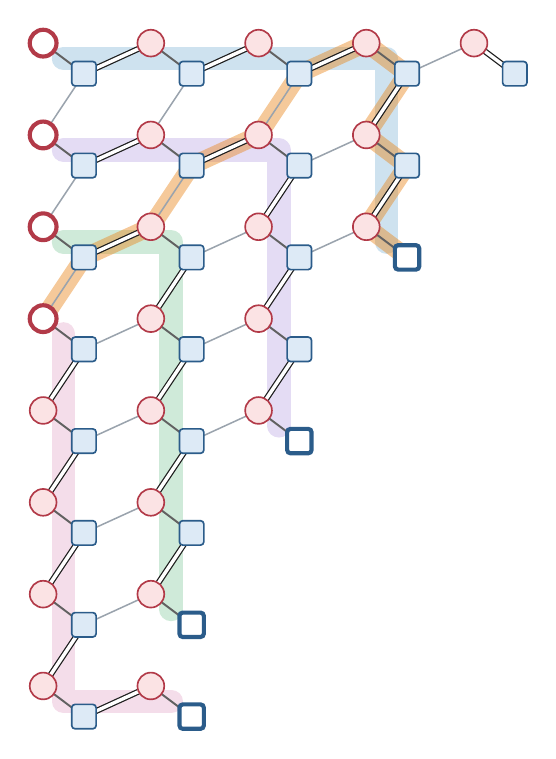
\begin{tikzpicture}[]
\begin{scope}[on background layer]
\draw[hook,rowA] (0.000,0.000) -- (1.368,0.000) -- (2.736,0.000) -- (4.104,0.000) -- (4.104,-1.166) -- (4.104,-2.333);
\draw[hook,rowB] (0.000,-1.166) -- (1.368,-1.166) -- (2.736,-1.166) -- (2.736,-2.333) -- (2.736,-3.499) -- (2.736,-4.666);
\draw[hook,rowC] (0.000,-2.333) -- (1.368,-2.333) -- (1.368,-3.499) -- (1.368,-4.666) -- (1.368,-5.832) -- (1.368,-6.998);
\draw[hook,rowD] (0.000,-3.499) -- (0.000,-4.666) -- (0.000,-5.832) -- (0.000,-6.998) -- (0.000,-8.165) -- (1.368,-8.165);
\draw[sap] (-0.259,-3.305) -- (0.259,-2.527) -- (1.109,-2.138) -- (1.627,-1.361) -- (2.477,-0.972) -- (2.995,-0.194) -- (3.845,0.194) -- (4.363,-0.194) -- (3.845,-0.972) -- (4.363,-1.361) -- (3.845,-2.138) -- (4.363,-2.527);
\end{scope}
\draw[couple] (-0.259,-7.970) -- (0.259,-7.193);
\draw[pedge] (-0.259,-7.970) -- (0.259,-8.359);
\draw[couple] (-0.259,-6.804) -- (0.259,-6.026);
\draw[pedge] (-0.259,-6.804) -- (0.259,-7.193);
\draw[couple] (-0.259,-5.638) -- (0.259,-4.860);
\draw[pedge] (-0.259,-5.638) -- (0.259,-6.026);
\draw[couple] (-0.259,-4.471) -- (0.259,-3.694);
\draw[pedge] (-0.259,-4.471) -- (0.259,-4.860);
\draw[edge] (-0.259,-3.305) -- (0.259,-2.527);
\draw[pedge] (-0.259,-3.305) -- (0.259,-3.694);
\draw[edge] (-0.259,-2.138) -- (0.259,-1.361);
\draw[pedge] (-0.259,-2.138) -- (0.259,-2.527);
\draw[edge] (-0.259,-0.972) -- (0.259,-0.194);
\draw[pedge] (-0.259,-0.972) -- (0.259,-1.361);
\draw[pedge] (-0.259,0.194) -- (0.259,-0.194);
\draw[couple] (1.109,0.194) -- (0.259,-0.194);
\draw[pedge] (1.109,0.194) -- (1.627,-0.194);
\draw[couple] (2.477,0.194) -- (1.627,-0.194);
\draw[pedge] (2.477,0.194) -- (2.995,-0.194);
\draw[couple] (3.845,0.194) -- (2.995,-0.194);
\draw[pedge] (3.845,0.194) -- (4.363,-0.194);
\draw[edge] (5.213,0.194) -- (4.363,-0.194);
\draw[couple] (5.213,0.194) -- (5.731,-0.194);
\draw[couple] (1.109,-0.972) -- (0.259,-1.361);
\draw[edge] (1.109,-0.972) -- (1.627,-0.194);
\draw[pedge] (1.109,-0.972) -- (1.627,-1.361);
\draw[couple] (2.477,-0.972) -- (1.627,-1.361);
\draw[edge] (2.477,-0.972) -- (2.995,-0.194);
\draw[pedge] (2.477,-0.972) -- (2.995,-1.361);
\draw[edge] (3.845,-0.972) -- (2.995,-1.361);
\draw[couple] (3.845,-0.972) -- (4.363,-0.194);
\draw[pedge] (3.845,-0.972) -- (4.363,-1.361);
\draw[couple] (1.109,-2.138) -- (0.259,-2.527);
\draw[edge] (1.109,-2.138) -- (1.627,-1.361);
\draw[pedge] (1.109,-2.138) -- (1.627,-2.527);
\draw[edge] (2.477,-2.138) -- (1.627,-2.527);
\draw[couple] (2.477,-2.138) -- (2.995,-1.361);
\draw[pedge] (2.477,-2.138) -- (2.995,-2.527);
\draw[edge] (3.845,-2.138) -- (2.995,-2.527);
\draw[couple] (3.845,-2.138) -- (4.363,-1.361);
\draw[pedge] (3.845,-2.138) -- (4.363,-2.527);
\draw[edge] (1.109,-3.305) -- (0.259,-3.694);
\draw[couple] (1.109,-3.305) -- (1.627,-2.527);
\draw[pedge] (1.109,-3.305) -- (1.627,-3.694);
\draw[edge] (2.477,-3.305) -- (1.627,-3.694);
\draw[couple] (2.477,-3.305) -- (2.995,-2.527);
\draw[pedge] (2.477,-3.305) -- (2.995,-3.694);
\draw[edge] (1.109,-4.471) -- (0.259,-4.860);
\draw[couple] (1.109,-4.471) -- (1.627,-3.694);
\draw[pedge] (1.109,-4.471) -- (1.627,-4.860);
\draw[edge] (2.477,-4.471) -- (1.627,-4.860);
\draw[couple] (2.477,-4.471) -- (2.995,-3.694);
\draw[pedge] (2.477,-4.471) -- (2.995,-4.860);
\draw[edge] (1.109,-5.638) -- (0.259,-6.026);
\draw[couple] (1.109,-5.638) -- (1.627,-4.860);
\draw[pedge] (1.109,-5.638) -- (1.627,-6.026);
\draw[edge] (1.109,-6.804) -- (0.259,-7.193);
\draw[couple] (1.109,-6.804) -- (1.627,-6.026);
\draw[pedge] (1.109,-6.804) -- (1.627,-7.193);
\draw[couple] (1.109,-7.970) -- (0.259,-8.359);
\draw[pedge] (1.109,-7.970) -- (1.627,-8.359);
\node[small girl] at (-0.259,-7.970) {};
\node[small girl] at (-0.259,-6.804) {};
\node[small girl] at (-0.259,-5.638) {};
\node[small girl] at (-0.259,-4.471) {};
\node[small girl,free] at (-0.259,-3.305) {};
\node[small girl,free] at (-0.259,-2.138) {};
\node[small girl,free] at (-0.259,-0.972) {};
\node[small girl,free] at (-0.259,0.194) {};
\node[small girl] at (1.109,0.194) {};
\node[small girl] at (2.477,0.194) {};
\node[small girl] at (3.845,0.194) {};
\node[small girl] at (5.213,0.194) {};
\node[small girl] at (1.109,-0.972) {};
\node[small girl] at (2.477,-0.972) {};
\node[small girl] at (3.845,-0.972) {};
\node[small girl] at (1.109,-2.138) {};
\node[small girl] at (2.477,-2.138) {};
\node[small girl] at (3.845,-2.138) {};
\node[small girl] at (1.109,-3.305) {};
\node[small girl] at (2.477,-3.305) {};
\node[small girl] at (1.109,-4.471) {};
\node[small girl] at (2.477,-4.471) {};
\node[small girl] at (1.109,-5.638) {};
\node[small girl] at (1.109,-6.804) {};
\node[small girl] at (1.109,-7.970) {};
\node[small boy] at (0.259,-0.194) {};
\node[small boy] at (1.627,-0.194) {};
\node[small boy] at (2.995,-0.194) {};
\node[small boy] at (4.363,-0.194) {};
\node[small boy] at (5.731,-0.194) {};
\node[small boy] at (0.259,-1.361) {};
\node[small boy] at (1.627,-1.361) {};
\node[small boy] at (2.995,-1.361) {};
\node[small boy] at (4.363,-1.361) {};
\node[small boy] at (0.259,-2.527) {};
\node[small boy] at (1.627,-2.527) {};
\node[small boy] at (2.995,-2.527) {};
\node[small boy,free] at (4.363,-2.527) {};
\node[small boy] at (0.259,-3.694) {};
\node[small boy] at (1.627,-3.694) {};
\node[small boy] at (2.995,-3.694) {};
\node[small boy] at (0.259,-4.860) {};
\node[small boy] at (1.627,-4.860) {};
\node[small boy,free] at (2.995,-4.860) {};
\node[small boy] at (0.259,-6.026) {};
\node[small boy] at (1.627,-6.026) {};
\node[small boy] at (0.259,-7.193) {};
\node[small boy,free] at (1.627,-7.193) {};
\node[small boy] at (0.259,-8.359) {};
\node[small boy,free] at (1.627,-8.359) {};
\end{tikzpicture}
}

\vfill
{\large Claude Opus 5.5\par}
\vspace{4mm}
{\small 3 November 2026\\[2pt]
References are to the pre-fascicle of 18 September 2026 (zeroth printing, revision~$-88$)\par}
\end{titlepage}

\pagenumbering{roman}
\begin{abstract}
\noindent
Knuth's Algorithm~7.5.1H (Algorithm~H for short), his implementation of
the Hopcroft--Karp algorithm, works in \emph{rounds}: each round builds a dag of shortest augmenting
paths and then removes a maximal set of disjoint ones. Exercise~15 of
Pre-Fascicle~14A asks how badly this can go, and proposes a candidate
worst case, the \emph{Tchoukaillon graph}, whose number of rounds is
governed by the Tchoukaillon numbers $\Ch_n\approx n^2/\pi$. These notes
answer the unrestricted version of the question, which the answer to
exercise~16 poses as harder. A graph whose maximum matching has
size~$s$ can force at most $\lfloor\sqrt{4s+1}\rfloor-1$ rounds, and this
is attained for every~$s$ by explicit \emph{staircase graphs}: planar
graphs of maximum degree three, with input orders under which we can
prove exactly what Algorithm~H does. Equivalently, $n$ rounds are possible
exactly when $s\ge\lfloor(n+1)^2/4\rfloor$. The smallest size at
which this beats a Tchoukaillon graph is $s=9$, and the advantage grows
like $(2-\sqrt\pi)\sqrt s$. On the same graphs Algorithm~H performs
$\Theta(E\sqrt V)$ operations. We also show that the literal definition
in exercise~15 can be met only when $s\in\{1,2,3,4,5,8,9\}$; Knuth's own
16-pair example meets a weaker condition, which we make precise. Whether
that weaker condition can be met for every $s$ is still open, and we
collect what is known about it.
\end{abstract}

\vspace{4mm}
\tableofcontents
\clearpage
\pagenumbering{arabic}

\section{Overview}
\label{sec:overview}

Algorithm~7.5.1H, in Knuth's Pre-Fascicle~14A~\cite{Knuth}, is his
implementation of the Hopcroft--Karp algorithm~\cite{HK}. Inside
Section~7.5.1 Knuth calls it simply Algorithm~H, and so shall we. After a
greedy start (step~\Hs1)
it repeats a \emph{round}: build a dag that contains every shortest
augmenting path, then dismantle the dag, augmenting along a maximal
collection of vertex-disjoint shortest paths. Corollary~K bounds the
number of rounds by about $2\sqrt s$, where $s$ is the size of a maximum
matching, so the running time is $O\bigl((M+N+E)\sqrt s\,\bigr)$.

Is that square root ever needed? Knuth remarks on page~5 that graphs
needing anywhere near $\sqrt s$ rounds are hard to find, and that even
for such a graph ``its edges have to appear in a particularly perverse
order.''
Exercise~15 proposes a candidate: a \emph{Tchoukaillon graph}, on which
each round removes as few shortest paths as a simple counting argument
allows. The resulting round count is governed by the Tchoukaillon
numbers $\Ch_n$ of exercise~11, and since $\Ch_n\approx n^2/\pi$, such a
graph would force about $\sqrt{\pi s}$ rounds. Exercise~16 asks whether
Tchoukaillon graphs exist for every~$s$, and its answer raises an even
harder question: can some graph force \emph{more} rounds than a
Tchoukaillon graph would? Fig.~\ref{fig:rounds} shows the answer.

\begin{figure}[ht]
\centering
\begin{tikzpicture}
\begin{axis}[
  width=.92\linewidth, height=6.4cm,
  xmin=0.5, xmax=64.5, ymin=0, ymax=16,
  xtick={1,9,16,25,36,49,64}, ytick={2,4,...,16},
  xlabel={size $s$ of a maximum matching}, ylabel={rounds},
  axis lines=left, tick style={black!50}, tick label style={font=\scriptsize},
  label style={font=\small},
  ymajorgrids, grid style={black!8},
  legend style={draw=none,fill=white,fill opacity=.85,text opacity=1,
    at={(0.5,-0.24)},anchor=north,legend columns=2,font=\small,cells={anchor=west},/tikz/every even column/.append style={column sep=6mm}},
  clip=false]
\fill[sapcol!18] (axis cs:8.5,0) rectangle (axis cs:9.5,16);
\fill[sapcol!18] (axis cs:15.5,0) rectangle (axis cs:16.5,16);
\fill[sapcol!18] (axis cs:16.5,0) rectangle (axis cs:17.5,16);
\fill[sapcol!18] (axis cs:19.5,0) rectangle (axis cs:20.5,16);
\fill[sapcol!18] (axis cs:20.5,0) rectangle (axis cs:21.5,16);
\fill[sapcol!18] (axis cs:24.5,0) rectangle (axis cs:25.5,16);
\fill[sapcol!18] (axis cs:25.5,0) rectangle (axis cs:26.5,16);
\fill[sapcol!18] (axis cs:26.5,0) rectangle (axis cs:27.5,16);
\fill[sapcol!18] (axis cs:27.5,0) rectangle (axis cs:28.5,16);
\fill[sapcol!18] (axis cs:28.5,0) rectangle (axis cs:29.5,16);
\fill[sapcol!18] (axis cs:29.5,0) rectangle (axis cs:30.5,16);
\fill[sapcol!18] (axis cs:30.5,0) rectangle (axis cs:31.5,16);
\fill[sapcol!18] (axis cs:31.5,0) rectangle (axis cs:32.5,16);
\fill[sapcol!18] (axis cs:32.5,0) rectangle (axis cs:33.5,16);
\fill[sapcol!18] (axis cs:35.5,0) rectangle (axis cs:36.5,16);
\fill[sapcol!18] (axis cs:36.5,0) rectangle (axis cs:37.5,16);
\fill[sapcol!18] (axis cs:37.5,0) rectangle (axis cs:38.5,16);
\fill[sapcol!18] (axis cs:38.5,0) rectangle (axis cs:39.5,16);
\fill[sapcol!18] (axis cs:39.5,0) rectangle (axis cs:40.5,16);
\fill[sapcol!18] (axis cs:40.5,0) rectangle (axis cs:41.5,16);
\fill[sapcol!18] (axis cs:41.5,0) rectangle (axis cs:42.5,16);
\fill[sapcol!18] (axis cs:42.5,0) rectangle (axis cs:43.5,16);
\fill[sapcol!18] (axis cs:43.5,0) rectangle (axis cs:44.5,16);
\fill[sapcol!18] (axis cs:44.5,0) rectangle (axis cs:45.5,16);
\fill[sapcol!18] (axis cs:45.5,0) rectangle (axis cs:46.5,16);
\fill[sapcol!18] (axis cs:46.5,0) rectangle (axis cs:47.5,16);
\fill[sapcol!18] (axis cs:48.5,0) rectangle (axis cs:49.5,16);
\fill[sapcol!18] (axis cs:49.5,0) rectangle (axis cs:50.5,16);
\fill[sapcol!18] (axis cs:50.5,0) rectangle (axis cs:51.5,16);
\fill[sapcol!18] (axis cs:51.5,0) rectangle (axis cs:52.5,16);
\fill[sapcol!18] (axis cs:52.5,0) rectangle (axis cs:53.5,16);
\fill[sapcol!18] (axis cs:53.5,0) rectangle (axis cs:54.5,16);
\fill[sapcol!18] (axis cs:54.5,0) rectangle (axis cs:55.5,16);
\fill[sapcol!18] (axis cs:55.5,0) rectangle (axis cs:56.5,16);
\fill[sapcol!18] (axis cs:56.5,0) rectangle (axis cs:57.5,16);
\fill[sapcol!18] (axis cs:57.5,0) rectangle (axis cs:58.5,16);
\fill[sapcol!18] (axis cs:58.5,0) rectangle (axis cs:59.5,16);
\fill[sapcol!18] (axis cs:63.5,0) rectangle (axis cs:64.5,16);

\addplot[const plot mark mid,qcol,line width=1.3pt,mark=none,restrict x to domain=0:64.6]
  table[x=s,y=R]{figures/gen_rounds.dat};
\addlegendentry{$R(s)=\floor{\sqrt{4s+1}}-1$, the true maximum}
\addplot[const plot mark mid,chcol,line width=1.1pt,mark=none,densely dashed,restrict x to domain=0:64.6]
  table[x=s,y=T]{figures/gen_rounds.dat};
\addlegendentry{$T(s)$, a Tchoukaillon graph}
\node[font=\scriptsize,sapcol!80!black,anchor=south] at (axis cs:9,16) {$s=9$};
\end{axis}
\end{tikzpicture}

\caption{The largest possible number of rounds~$R(s)$ (blue), against
the number of rounds~$T(s)$ that a Tchoukaillon graph would need (red),
for matching sizes~$s\le64$. Shaded columns mark the sizes where
$R(s)>T(s)$; the first is $s=9$. The two staircases step up at the
quarter-squares $Q_n$ and at the Tchoukaillon numbers $\Ch_n$
(both defined below).}
\label{fig:rounds}
\end{figure}

\subsection*{The answers in brief}

\begin{summarybox}
\begin{enumerate}[leftmargin=1.4em,label=\textbf{\arabic*.}]
\item \textbf{The maximum number of rounds.} Count~\Hs1 as the first
round, as answer~15(c) does. A bipartite graph whose maximum matching
has $s$ edges can make Algorithm~H perform at most
\[
   R(s)=\bigfloor{\sqrt{4s+1}}-1
\]
rounds, whatever the order of its input, and for every $s$ some graph
and input order attain this bound (Theorem~R). Put differently,
$n$ rounds are possible exactly when
\[
   s\ \ge\ Q_n=\bigfloor{\frac{(n+1)^2}4}\qquad(\text{the quarter-squares }1,2,4,6,9,12,16,20,\ldots),
\]
while a hypothetical Tchoukaillon graph has at least $n$ rounds exactly
when $s\ge\Ch_n$ $(1,2,4,6,10,12,18,22,\ldots)$.
\item \textbf{Staircase graphs.} The extremal graphs are explicit, planar,
and have maximum degree three. Their input orders make Algorithm~H
find exactly one shortest augmenting path per round, at levels
$L=2,3,\ldots,n$, and we can prove every step of the execution
(Theorem~S). Algorithm~H performs $\Theta(E\sqrt V)$ elementary operations
on them (Theorem~W), so Corollary~K is tight even for sparse planar graphs.
\item \textbf{Beating Tchoukaillon.} Always $Q_n\le\Ch_n$, so the true
worst case is always at least as slow as a Tchoukaillon graph would be.
The first size where it is strictly slower is $s=9$: five rounds are
possible, against four. Asymptotically $R(s)-T(s)\sim(2-\sqrt\pi)\sqrt s$
(Section~\ref{sec:comparison}).
\item \textbf{The literal definition.} Exercise~15(c) asks that
\emph{every} augmenting path have the current shortest level at every
round. Graphs meeting that requirement exist only when
$s\in\{1,2,3,4,5,8,9\}$ (Corollary~L), because consecutive rounds of this
kind must at least halve the number of free girls (Theorem~U). Knuth's
16-pair example in answer~15(d) has augmenting paths of levels~2 and~3
immediately after~\Hs1, yet with suitable input orders it does follow
the Tchoukaillon schedule.
\item \textbf{The open question.} Can the Tchoukaillon \emph{schedule} (the
numbers of free girls and of paths removed, round by round) be realized
for every $s$? Explicit inputs exist for all $s\le47$, and they even keep
$f$ disjoint SAPs in every round, as Knuth's matrices do. Any family of
inputs that realizes the schedule for unboundedly large $s$ must contain
at least $s/12-O(1)$ independent cycles (Theorem~C). Some candidate graphs
fail only because of the order in which Algorithm~H searches: its queue,
the head insertion of step~\Hs6, and the replacement rule of step~\Hs{16}
(Section~\ref{sec:order}).
\end{enumerate}
\end{summarybox}

\subsection*{How these notes are organized}

Section~\ref{sec:background} recalls just enough of Algorithm~H to make
precise what an ``input'' is and which choices it leaves open; it
also works through one round of an example that recurs throughout.
Section~\ref{sec:ex15} restates exercise~15, explains where the
Tchoukaillon numbers come from, and separates three ways of reading the
definition of a Tchoukaillon graph. Sections~\ref{sec:upper}
and~\ref{sec:staircase} prove Theorem~R: first the upper bound, which is
a sharpened form of the counting in Theorem~H, then the staircase
construction. Section~\ref{sec:comparison} compares the answer with the
Tchoukaillon numbers. Section~\ref{sec:literal} settles the literal
reading of exercise~15, and Section~\ref{sec:operational} collects what
we know about the open, numerical reading. Section~\ref{sec:sparse}
gives simpler examples for the running-time question alone.
Section~\ref{sec:credits} discusses the literature.

The appendices give a complete ordered input for Knuth's 16-pair graph,
details of a family that meets the literal definition, a catalog of
computed examples, and a guide to the accompanying programs.

\paragraph{Which draft.} Page, exercise, step, and equation numbers refer
to the zeroth printing of Pre-Fascicle~14A, revision~$-88$, dated
18~September 2026. A pre-fascicle is a working draft, so these numbers may
change in later revisions.

\subsection*{What is classical and what is new}

The tools are the ones in the pre-fascicle: Berge's augmenting paths
\cite{Berge}, the layered dag and the fact that the shortest level
increases from round to round~\cite{HK}, and the counting argument
behind Theorem~H. The upper bound in Theorem~R refines Hopcroft and Karp's
bound on the number of phases. As far as we know, the staircase graphs,
the exact value of $R(s)$, and the results of Sections~\ref{sec:literal}
and~\ref{sec:operational}, are new; Section~\ref{sec:credits} discusses
the literature.

\section{Algorithm H in brief}
\label{sec:background}

This section recalls the parts of Section~7.5.1 that matter for worst
cases. Readers who know pages~1--5 of the pre-fascicle well can skim it,
but should look at two things: the definition of an \emph{input} in
Section~\ref{sec:input}, which fixes exactly what freedom a worst-case
construction has, and the worked round in Section~\ref{sec:worked}.

\subsection{Matchings and augmenting paths}

A bipartite graph has $M$ \emph{girls} and $N$ \emph{boys}, joined by $E$
edges; each edge joins a girl to a boy. A \emph{matching} is a set of
edges with no common vertex. Its edges are called \emph{couples}, and a
vertex that belongs to no couple is \emph{free}. A matching is
\emph{maximal} if no edge can be added to it, and \emph{maximum} if no
matching has more edges. Throughout, $s$ denotes the size of a maximum
matching. We often write $V=M+N$ for the number of vertices.

We follow the pre-fascicle's drawing conventions. When two matchings are
compared, an edge of the reference matching is written $x\sg y$ and an
edge of the current matching $M'$ is written $x\db y$. In particular an
\emph{augmenting path} for $M'$ is a path
\begin{equation}
  g_0\sg b_1\db g_1\sg b_2\db\cdots\db g_{L-1}\sg b_L
  \label{eq:augpath}
\end{equation}
that starts at a free girl, ends at a free boy, and alternates between
edges outside and inside $M'$. It has $2L-1$ edges, and we say it has
\emph{level}~$L$. Exchanging the two kinds of edges along the path
(Fig.~\ref{fig:augpath}) produces a matching with one more couple.
In~\eqref{eq:augpath} no reference matching is involved, and the single
lines mean ``an edge not in~$M'$.'' We describe augmenting paths by
their level; when the number of edges matters we say so. An edge named
without regard to any matching is written by juxtaposition, as in
$g_1b_6$.

\begin{figure}[ht]
\centering
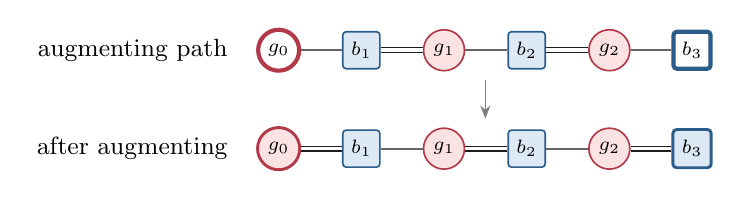
\begin{tikzpicture}[x=1.05cm]
\foreach \row/\y/\name in {0/0/before,1/-1.25/after}{
  \node[girl,free] (g0\row) at (0,\y) {$g_0$};
  \node[boy] (b1\row) at (1,\y) {$b_1$};
  \node[girl] (g1\row) at (2,\y) {$g_1$};
  \node[boy] (b2\row) at (3,\y) {$b_2$};
  \node[girl] (g2\row) at (4,\y) {$g_2$};
  \node[boy,free] (b3\row) at (5,\y) {$b_3$};
}
\draw[edge,line width=.8pt,draw=black!60] (g00)--(b10) (g10)--(b20) (g20)--(b30);
\draw[couple] (b10)--(g10) (b20)--(g20);
\draw[couple] (g01)--(b11) (g11)--(b21) (g21)--(b31);
\draw[edge,line width=.8pt,draw=black!60] (b11)--(g11) (b21)--(g21);
\node[girl] at (g01) {$g_0$};\node[boy] at (b31) {$b_3$};
\node[anchor=east,font=\small] at (-.5,0) {augmenting path};
\node[anchor=east,font=\small] at (-.5,-1.25) {after augmenting};
\draw[-{Stealth},black!50] (2.5,-.38)--(2.5,-.87);
\end{tikzpicture}

\caption{An augmenting path of level~$L=3$, and the matching after
augmenting along it. Double lines are couples; heavy outlines mark free
vertices. In all figures girls are drawn as circles and boys as squares.}
\label{fig:augpath}
\end{figure}

Berge's observation~\cite{Berge} (pre-fascicle, page~1) is that if $M'$ has
$s'$ couples, then the union of $M'$ with a maximum matching contains at
least $s-s'$ \emph{vertex-disjoint} augmenting paths for $M'$. We shall
use this mostly when $s=M=N$, so that there is a \emph{perfect}
matching~$P$. Then the symmetric difference $M'\symdiff P$ consists of
exactly $f$ vertex-disjoint augmenting paths, where $f=M-s'$ is the number
of free girls, together with some alternating cycles. Following answer
15(a), we call these $f$ paths the \emph{basic paths} of $M'$ with
respect to~$P$. A basic path of level~$\ell$ contains exactly $\ell$ edges
of~$P$, and like Knuth in answer~15(d) we often draw it as a \emph{row} of
$\ell$ cells, one for each girl--boy pair of~$P$ that it visits. (Later
sections call these rows the rows of a matrix, or hooks; they are always
basic paths.)

\subsection{Shortest augmenting paths and rounds}
\label{sec:dag}

A \emph{shortest augmenting path}, or SAP, is an augmenting path of
smallest level. To find them, orient every edge relative to the current
matching: an edge outside the matching points from its girl to its boy,
and a couple points from its boy to its girl. Alternating paths that start
at a free girl are then exactly the directed paths that start there. The
\emph{distance} of a vertex is the number of edges on a shortest such
directed path from some free girl to it.

Hopcroft and Karp~\cite{HK} organize all SAPs into a directed acyclic
graph, built breadth-first from the free girls (page~2 of the
pre-fascicle). The dag has \emph{levels} $G_0,B_1,G_1,\ldots,
G_{L-1},B_L$: $G_0$ is the set of free girls; $B_k$ consists of the
boys first reached from girls in $G_{k-1}$; and $G_k$ consists of the
mates of the boys in $B_k$. So $G_k$ and $B_k$ are the girls at distance
$2k$ and the boys at distance $2k-1$. There is an arc $b\to g$ for each edge
$g\sg b$ with $g\in G_{k-1}$, $b\in B_k$, and an arc from each girl to
her mate. The construction stops at the first level~$B_L$ that contains
a free boy. Knuth adds two special nodes: arcs $g\to\bot$ from the free
girls and $\top\to b$ to the free boys of~$B_L$. The SAPs are then
exactly the paths from $\top$ to $\bot$, read backwards; this is why the
arcs in the pre-fascicle's figure~(7) point to the left.

Each \emph{round} of Algorithm~H builds this dag (steps~\Hs2--\Hs{10})
and then dismantles it (steps~\Hs{11}--\Hs{17}): it repeatedly finds a
path from $\top$ to $\bot$ by depth-first search, augments the matching
along it, and deletes its vertices from the dag. When no path remains,
the paths removed form a \emph{maximal} set of vertex-disjoint SAPs:
no further SAP is disjoint from all of them. This set need not be as
large as possible, and the gap between ``maximal'' and ``maximum'' is
what a worst-case input exploits.

After a round at level~$L$, every augmenting path has level greater
than~$L$; this is exercise~5, and goes back to Hopcroft and Karp
\cite[Theorem~2 and Corollaries~3--4]{HK}. So the levels of successive rounds strictly
increase. Theorem~H turns this into a
counting bound: when a round at level~$L$ is over, every one of the
$s-s'$ disjoint augmenting paths has at least $L+1$ edges of a maximum
matching, so $s\ge(L+1)(s-s')$. Corollary~K deduces that there are at
most about $2\sqrt s$ rounds, each costing $O(M+N+E)$.

\subsection{What an input is}
\label{sec:input}

Algorithm~H is deterministic. To speak of a graph that ``might cause''
it to behave badly, as exercise~15(c) does, we must say exactly which
features of the input it reads. There are two:
\begin{enumerate}[label=(\roman*)]
\item the numbering of the girls~$1,\ldots,M$, which fixes the order in
  which step~\Hs1 scans them;
\item for each girl~$g$, the order of her list of boys, which starts at
  $\A{GLINK}[g]$ and continues through $\A{GNEXT}$.
\end{enumerate}
We call a bipartite graph together with these data an \emph{ordered
graph}. By exercise~6, any desired list order arises from a suitable
order of the input pairs, since each new edge is inserted at the front
of its girl's list. Nothing else matters. The numbering of the boys is
irrelevant, since no step compares boy indices. There is also \emph{no}
boy-side order to choose: the reverse lists $\A{BLINK}[b]$ are built by
the algorithm itself.

For orientation, here is what the steps do, in our words (the precise
code is on pages~4--5 of the pre-fascicle).
\begin{center}\small
\begin{tabular}{@{}>{\raggedright\arraybackslash}p{.17\textwidth}>{\raggedright\arraybackslash}p{.76\textwidth}@{}}
\toprule
\Hs1&Greedy start: a maximal matching; the free girls go into \A{QUEUE}.\\
\Hs2--\Hs3&Start a dag; start the next level.\\
\Hs4--\Hs7&Take the next girl of the current level and scan her list of boys.\\
\Hs8--\Hs9&A boy seen for the first time joins the next level; his mate is
  queued for the level after, or, if he is free, the final level~$L$ is
  fixed and he is recorded as a root.\\
\Hs{10}&Go on to the next level, or finish the dag (or stop if no free boy was reached).\\
\Hs{11}&Take the next root; if none is left, reset all marks and start a new round.\\
\Hs{12}--\Hs{15}&Depth-first search from the root down the reverse lists
  \A{BLINK}, consuming each arc it follows and skipping used girls;
  back up when a list runs out.\\
\Hs{16}--\Hs{17}&A free girl was reached: remove her from the free list and
  augment along the path.\\
\bottomrule
\end{tabular}
\end{center}

The following consequences of the code will be used repeatedly.

\begin{itemize}
\item \textbf{\Hs1 scans the girls in decreasing order.} Answer~7 matches
  girl~$g$ to the first free boy on her list, for $g=M,M-1,\ldots,1$,
  and appends each unsuccessful girl to \A{QUEUE}. So the free girls
  start out in \A{QUEUE} in decreasing numerical order. The resulting
  matching is maximal, so the first dag has $L\ge2$.
\item \textbf{The dag levels are scanned in queue order.} Girls of $G_l$
  are processed in their order in \A{QUEUE}; each scans her own list in
  order. A boy enters $B_{l+1}$ when he is first seen (step~\Hs8), and
  his mate is appended to \A{QUEUE} as a girl of $G_{l+1}$ (step
  \Hs9). So the order of $G_{l+1}$ is the order in which the boys of
  $B_{l+1}$ were discovered.
\item \textbf{Reverse lists are built by insertion at the head.} The
  first girl who sees $b$ becomes the only entry of $\A{BLINK}[b]$
  (step~\Hs8); every later girl of the same level who is adjacent to $b$
  is inserted at the \emph{front} (step~\Hs6). Hence $\A{BLINK}[b]$ lists
  the girls of $G_l$ adjacent to $b$ in the \emph{reverse} of their order
  in \A{QUEUE}.
\item \textbf{The last level is cut short.} When the first free boy is
  found, $L$ is set to the current level and the queue of the next
  level is discarded. After that, matched boys are no longer entered
  (step~\Hs8), but free boys still are. The free boys of $B_L$ are the
  last $r$ entries of \A{MARKED}, in order of discovery, and step~\Hs{11}
  uses them as roots of the depth-first search in that order.
\item \textbf{The depth-first search destroys what it reads.} Step~\Hs{13}
  removes each arc from $\A{BLINK}[b]$ as it follows it, and skips a
  girl if she has already been used by an earlier SAP of this round
  (she is ``deleted''). If a list becomes empty, step~\Hs{15} backs up
  one level; nothing is ever re-examined. Reaching a free girl completes
  a SAP.
\item \textbf{A used free girl is replaced by the last one.} Step~\Hs{16}
  removes the girl~$g_0$ of a new SAP from the free list by moving the
  last free girl, $\A{QUEUE}[f-1]$, into her slot. So the order of the
  free girls is preserved only if each SAP ends at the last of them.
\end{itemize}

\subsection{A worked round}
\label{sec:worked}

The ordered graph of Fig.~\ref{fig:gamma5} has nine girls and nine
boys. Its girl lists, in increasing order of girls, are
\begin{equation}
  [6,8];\ [4,6];\ [1,4];\ [1];\ [1,2];\ [2,3];\ [4,2,5];\ [6,5,7];\ [8,9].
  \label{eq:gamma5lists}
\end{equation}
(Girl~1 is adjacent to boys~6 and~8, in that order, and so on.)
Its vertices are arranged in nine \emph{cells}: cell~$(a,c)$, in row~$a$
and column~$c$, holds one girl and one boy, joined by an edge (the short
dark edge inside the cell). These nine edges form a perfect matching, so
$s=9$. The other edges join the boy of a cell either to the girl of the
next cell in the same row or to the girl of the cell below; in the
drawing they run diagonally, up-right and down-left respectively. We
shall meet this graph again in Section~\ref{sec:staircase} as the
staircase graph~$\Gam_5$.

\begin{figure}[ht]
\centering
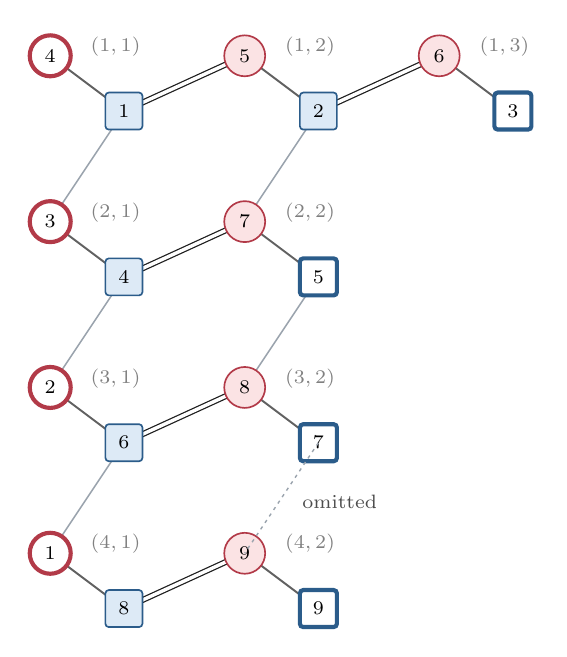
\begin{tikzpicture}[]
\begin{scope}[on background layer]
\end{scope}
\draw[edge] (-0.468,-5.967) -- (0.468,-4.563);
\draw[pedge] (-0.468,-5.967) -- (0.468,-6.669);
\draw[edge] (-0.468,-3.861) -- (0.468,-2.457);
\draw[pedge] (-0.468,-3.861) -- (0.468,-4.563);
\draw[edge] (-0.468,-1.755) -- (0.468,-0.351);
\draw[pedge] (-0.468,-1.755) -- (0.468,-2.457);
\draw[pedge] (-0.468,0.351) -- (0.468,-0.351);
\draw[couple] (2.002,0.351) -- (0.468,-0.351);
\draw[pedge] (2.002,0.351) -- (2.938,-0.351);
\draw[couple] (4.472,0.351) -- (2.938,-0.351);
\draw[pedge] (4.472,0.351) -- (5.408,-0.351);
\draw[couple] (2.002,-1.755) -- (0.468,-2.457);
\draw[edge] (2.002,-1.755) -- (2.938,-0.351);
\draw[pedge] (2.002,-1.755) -- (2.938,-2.457);
\draw[couple] (2.002,-3.861) -- (0.468,-4.563);
\draw[edge] (2.002,-3.861) -- (2.938,-2.457);
\draw[pedge] (2.002,-3.861) -- (2.938,-4.563);
\draw[couple] (2.002,-5.967) -- (0.468,-6.669);
\draw[pedge] (2.002,-5.967) -- (2.938,-6.669);
\node[girl,free] at (-0.468,-5.967) {1};
\node[girl,free] at (-0.468,-3.861) {2};
\node[girl,free] at (-0.468,-1.755) {3};
\node[girl,free] at (-0.468,0.351) {4};
\node[girl] at (2.002,0.351) {5};
\node[girl] at (4.472,0.351) {6};
\node[girl] at (2.002,-1.755) {7};
\node[girl] at (2.002,-3.861) {8};
\node[girl] at (2.002,-5.967) {9};
\node[boy] at (0.468,-0.351) {1};
\node[boy] at (2.938,-0.351) {2};
\node[boy,free] at (5.408,-0.351) {3};
\node[boy] at (0.468,-2.457) {4};
\node[boy,free] at (2.938,-2.457) {5};
\node[boy] at (0.468,-4.563) {6};
\node[boy,free] at (2.938,-4.563) {7};
\node[boy] at (0.468,-6.669) {8};
\node[boy,free] at (2.938,-6.669) {9};
\node[lab,font=\scriptsize,text=black!50,anchor=west] at (-0.078,0.468) {$(1,1)$};
\node[lab,font=\scriptsize,text=black!50,anchor=west] at (2.392,0.468) {$(1,2)$};
\node[lab,font=\scriptsize,text=black!50,anchor=west] at (4.862,0.468) {$(1,3)$};
\node[lab,font=\scriptsize,text=black!50,anchor=west] at (-0.078,-1.638) {$(2,1)$};
\node[lab,font=\scriptsize,text=black!50,anchor=west] at (2.392,-1.638) {$(2,2)$};
\node[lab,font=\scriptsize,text=black!50,anchor=west] at (-0.078,-3.744) {$(3,1)$};
\node[lab,font=\scriptsize,text=black!50,anchor=west] at (2.392,-3.744) {$(3,2)$};
\node[lab,font=\scriptsize,text=black!50,anchor=west] at (-0.078,-5.850) {$(4,1)$};
\node[lab,font=\scriptsize,text=black!50,anchor=west] at (2.392,-5.850) {$(4,2)$};
\draw[edgecol,line width=.5pt,dash pattern=on 1.2pt off 1.6pt] (2.938,-4.563) -- (2.002,-5.967);
\node[lab,anchor=west,font=\scriptsize] at (2.610,-5.315) {omitted};
\end{tikzpicture}

\caption{The 9-pair example, with the matching produced by~\Hs1. The
grey label $(a,c)$ names the cell of the girl beside it and of the boy
below her; the dark edge joining them belongs to a perfect matching.
Light grey lines are the other edges of the graph, double lines are
couples, and free vertices have heavy outlines. The dotted segment
marks an edge deliberately left out of the graph
(Section~\ref{sec:gamma}).}
\label{fig:gamma5}
\end{figure}

\paragraph{Step H1.}
Girls~$9,8,7,6,5$ come first. Each takes the first boy on her list,
namely $8,6,4,2,1$, and these are all different. Girls~$4,3,2,1$ then
find every boy on their lists taken. So~\Hs1 produces the five couples
drawn as double lines in Fig.~\ref{fig:gamma5}, and
\[
   \A{QUEUE}=(4,3,2,1),\qquad f=4 .
\]
In the picture, the free girls are the first girls of the four rows,
and the free boys are the last boys of the rows.

\paragraph{Building the dag.}
Fig.~\ref{fig:gamma5dag} shows the dag of the first round. Girl~4 scans
her list $[1]$ and discovers boy~1. Girl~3 scans $[1,4]$: boy~1 has
already been seen at this level, so girl~3 is inserted at the head of
$\A{BLINK}[1]$, giving $\A{BLINK}[1]=(3,4)$; then she discovers boy~4.
Girls~2 and~1 behave the same way, so $B_1=\{1,4,6,8\}$ in that order,
and their mates $5,7,8,9$ form $G_1$. At the next level boy~2 is
discovered first; he is matched (to girl~6), so the construction goes
on. Then girl~7 discovers boy~5, who is free: now $L=2$. Boys~7 and~9
are free too, so the roots of the search will be $5,7,9$, in that
order.

\begin{figure}[ht]
\centering
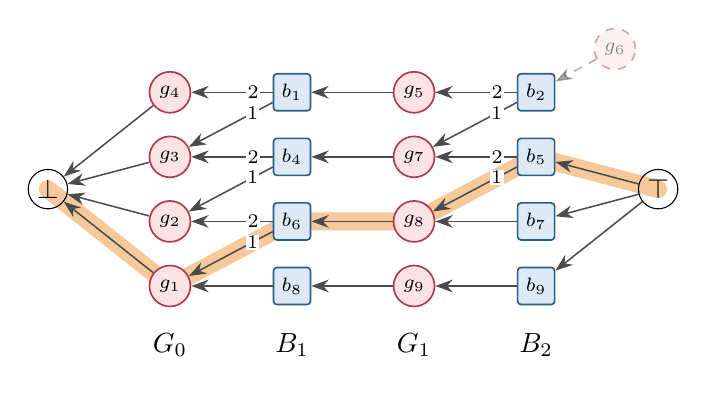
\begin{tikzpicture}[]
\begin{scope}[on background layer]
\draw[sap] (0.000,-1.230) -- (1.550,-2.460) -- (3.100,-1.640) -- (4.650,-1.640) -- (6.200,-0.820) -- (7.750,-1.230);
\end{scope}
\node[girl] (g4) at (1.550,0.000) {$g_{4}$};
\node[girl] (g3) at (1.550,-0.820) {$g_{3}$};
\node[girl] (g2) at (1.550,-1.640) {$g_{2}$};
\node[girl] (g1) at (1.550,-2.460) {$g_{1}$};
\node[boy] (b1) at (3.100,0.000) {$b_{1}$};
\node[boy] (b4) at (3.100,-0.820) {$b_{4}$};
\node[boy] (b6) at (3.100,-1.640) {$b_{6}$};
\node[boy] (b8) at (3.100,-2.460) {$b_{8}$};
\node[girl] (g5) at (4.650,0.000) {$g_{5}$};
\node[girl] (g7) at (4.650,-0.820) {$g_{7}$};
\node[girl] (g8) at (4.650,-1.640) {$g_{8}$};
\node[girl] (g9) at (4.650,-2.460) {$g_{9}$};
\node[boy] (b2) at (6.200,0.000) {$b_{2}$};
\node[boy] (b5) at (6.200,-0.820) {$b_{5}$};
\node[boy] (b7) at (6.200,-1.640) {$b_{7}$};
\node[boy] (b9) at (6.200,-2.460) {$b_{9}$};
\node[circle,draw,inner sep=1pt,minimum size=5mm] (bot) at (0.000,-1.230) {$\bot$};
\node[circle,draw,inner sep=1pt,minimum size=5mm] (top) at (7.750,-1.230) {$\top$};
\node[girl,dashed,opacity=.45] (gx6) at (7.200,0.550) {$g_{6}$};
\draw[arc,dashed,opacity=.45] (gx6) -- (b2);
\draw[arc] (g4) -- (bot);
\draw[arc] (g3) -- (bot);
\draw[arc] (g2) -- (bot);
\draw[arc] (g1) -- (bot);
\draw[arc] (g5) -- (b1);
\draw[arc] (g7) -- (b4);
\draw[arc] (g8) -- (b6);
\draw[arc] (g9) -- (b8);
\draw[arc] (b1) -- node[pos=.24,fill=white,inner sep=.5pt,font=\scriptsize] {1} (g3);
\draw[arc] (b1) -- node[pos=.24,fill=white,inner sep=.5pt,font=\scriptsize] {2} (g4);
\draw[arc] (b4) -- node[pos=.24,fill=white,inner sep=.5pt,font=\scriptsize] {1} (g2);
\draw[arc] (b4) -- node[pos=.24,fill=white,inner sep=.5pt,font=\scriptsize] {2} (g3);
\draw[arc] (b6) -- node[pos=.24,fill=white,inner sep=.5pt,font=\scriptsize] {1} (g1);
\draw[arc] (b6) -- node[pos=.24,fill=white,inner sep=.5pt,font=\scriptsize] {2} (g2);
\draw[arc] (b8) --  (g1);
\draw[arc] (b2) -- node[pos=.24,fill=white,inner sep=.5pt,font=\scriptsize] {1} (g7);
\draw[arc] (b2) -- node[pos=.24,fill=white,inner sep=.5pt,font=\scriptsize] {2} (g5);
\draw[arc] (b5) -- node[pos=.24,fill=white,inner sep=.5pt,font=\scriptsize] {1} (g8);
\draw[arc] (b5) -- node[pos=.24,fill=white,inner sep=.5pt,font=\scriptsize] {2} (g7);
\draw[arc] (b7) --  (g8);
\draw[arc] (b9) --  (g9);
\draw[arc] (top) -- (b5);
\draw[arc] (top) -- (b7);
\draw[arc] (top) -- (b9);
\node at (1.550,-3.210) {$G_0$};
\node at (3.100,-3.210) {$B_1$};
\node at (4.650,-3.210) {$G_1$};
\node at (6.200,-3.210) {$B_2$};
\end{tikzpicture}

\caption{The first dag for the graph of Fig.~\ref{fig:gamma5}, drawn as
in the pre-fascicle's figure~(7). When a boy has two arcs, the small
numbers give their order in $\A{BLINK}$; the girl who discovered him
comes \emph{second}. The shaded path is the only SAP that Algorithm~H
finds. Boy~2 belongs to $B_2$ but is matched, so his mate (faded) is
not part of the dag.}
\label{fig:gamma5dag}
\end{figure}

\paragraph{Dismantling the dag.}
The search starts at boy~5. The head of his list is girl~8, whose mate
is boy~6; the head of $\A{BLINK}[6]$ is girl~1, who is free. That
completes the SAP
\[
    g_1\sg b_6\db g_8\sg b_5 ,
\]
and Algorithm~H augments along it. The next root, boy~7, has only
girl~8 on his list, and she has just been used. The last root, boy~9,
leads to girl~9 and then to boy~8, whose only remaining entry is
girl~1, also used. So the round ends with a \emph{single} SAP, even
though the four rows of Fig.~\ref{fig:gamma5} contain three disjoint
SAPs (rows~2, 3, and~4). The one path that was found meets all three
of them. Step~\Hs{16} removed girl~1, the last free girl, so the queue
for the next round is $(4,3,2)$.

The remaining rounds behave similarly: each finds one SAP, at levels
$3$, $4$, and $5$, so the whole run has five rounds counting~\Hs1.
Fig.~\ref{fig:gamma5rounds} on page~\pageref{fig:gamma5rounds} shows
all of them. A Tchoukaillon graph with $s=9$ would need only four.

\subsection{Counting rounds and operations}
\label{sec:counting}

Answer~15(c) gives the number of rounds of a Tchoukaillon graph as
``the final value of~$L$.'' In such a graph the dags have levels
$2,3,\ldots,L$, so this count treats step~\Hs1 as a round at level~1;
answer~7 makes the same identification when it notes that, if~\Hs1 did
not produce a maximal matching, the first round would do so with $L=1$.
We adopt this convention.

\begin{definition}
A round is \emph{successful} if it enlarges the matching. The
\emph{number of rounds} of a run of Algorithm~H is the number of
successful rounds, where step~\Hs1 counts as one round (successful
whenever the graph has an edge). The final dag construction, which
finds no augmenting path and stops the algorithm, is not counted.
\end{definition}

Thus a run on a graph with $s\ge1$ has $1+k$ rounds if $k$ dags contain
augmenting paths. If the levels of those dags are $2,3,\ldots,n$ then
there are exactly $n$ rounds. The run of Section~\ref{sec:worked} has
five.

For running times we count elementary operations of Algorithm~H rather
than seconds. In each successful round we record three counts, named
after the steps that perform them:
\begin{align*}
  W_5&=\text{number of adjacency entries examined in step~\Hs5 (the breadth-first search)},\\
  W_{13}&=\text{number of arcs consumed in step~\Hs{13} (the depth-first search)},\\
  W_{11}&=\text{number of marks reset in step~\Hs{11}, which equals the number of boys in the dag.}
\end{align*}
$W_{13}$ includes arcs that lead to deleted girls. Every other step of a
round costs $O(1)$ per unit of one of these counts, plus $O(f)$, so the
total work in rounds after~\Hs1 is $\Theta(W_5+W_{13}+W_{11})$ up to that
small additive term. For example, the round of Section~\ref{sec:worked}
has $W_5=17$ (girls~$4,3,2,1,5,7,8,9$ have lists of total length~17),
$W_{11}=8$ (the boys of $B_1$ and $B_2$), and $W_{13}=5$ (two arcs for the
successful root, one for boy~7, and two for boy~9).

\section{Exercise~15 and Tchoukaillon graphs}
\label{sec:ex15}

Exercise~15 assumes that the input has a perfect matching, $s=M=N$, and
looks for a graph on which $L$ increases by only~1 per round while each
round removes as few SAPs as possible. This section explains the
counting behind the exercise, where the Tchoukaillon numbers enter, and
why the definition of a Tchoukaillon graph can be read in more than one
way.

\subsection{Basic paths and parts (a) and (b)}

Fix a perfect matching $P$ and a current matching with $f$ free girls,
whose next dag has level~$L$. Recall that the basic paths are the $f$
vertex-disjoint augmenting paths in the symmetric difference of the
current matching with~$P$. We also need the number
\[
   \nu=\text{the largest number of vertex-disjoint SAPs of the current matching}.
\]
Always $\nu\le f$, since each SAP uses its own free girl.

\begin{lemma}[Exercise~15(a), (b)]
\label{lem:15ab}
\leavevmode
\begin{enumerate}[label=(\alph*)]
\item If every augmenting path of the current matching has level~$L$, then
  the dag satisfies
  \(f\le\min\{|G_0|,|B_1|,\ldots,|G_{L-1}|,|B_L|\}\).
\item Every maximal set of vertex-disjoint SAPs has at least
  $\ceil{\nu/(L+1)}$ members. In particular, if there are $f$
  vertex-disjoint SAPs (as there are under the hypothesis of~(a)), steps
  \Hs{11}--\Hs{17} find at least $\ceil{f/(L+1)}$ of them.
\end{enumerate}
\end{lemma}

\begin{proof}
(a) Under the hypothesis, the $f$ basic paths are SAPs. Let
$g_0\sg b_1\db g_1\sg\cdots\sg b_L$ be one of them. Its first part shows
that $g_j$ has distance at most~$2j$. If the distance were smaller, a
shortest directed path to $g_j$ followed by the rest of the SAP would be an
alternating walk from a free girl to a free boy with fewer than $2L-1$
edges; cutting out the closed loops of that walk would leave an
augmenting path of smaller level, which is impossible. So $g_j\in G_j$,
and likewise $b_j\in B_j$. Disjoint paths contribute different vertices
to each level.

(b) Let $S$ be a SAP. Its interior vertices are matched, and any
augmenting path through a matched vertex also contains that vertex's
mate. So a path that meets $S$ meets it at $g_0$, at $b_L$, or in one
of the $L-1$ couples of~$S$. Paths of a vertex-disjoint family can
share none of these, so $S$ meets at most $L+1$ members of the family.
Take a family of $\nu$ disjoint SAPs: each of them must meet some path of
the maximal set (otherwise it could be added), and the bound follows.
\end{proof}

The hypothesis of~(a) is stronger than what~(b) needs. This difference
between ``all augmenting paths have level~$L$'' and ``there are $f$
disjoint SAPs'' leads to the three readings of Section~\ref{sec:readings},
and the gap between $\nu$ and $f$ is what the worst cases of
Section~\ref{sec:staircase} exploit.

\subsection{The schedule and the Tchoukaillon numbers}
\label{sec:schedule}

A maximal matching has at least $\ceil{s/2}$ couples, because each of
the $s$ edges of $P$ must touch one of its couples and each couple
touches at most two of them. So~\Hs1 leaves at most $\floor{s/2}$ girls
free. Exercise~15(c) asks for a graph that starts with this largest
possible number of free girls and, at every level~$L=2,3,\ldots$,
removes only the number of SAPs that Lemma~\ref{lem:15ab}(b) forces when
$\nu=f$. The numbers of free girls and of SAPs removed then follow the
\emph{Tchoukaillon schedule}
\begin{equation}
  f_2=\floor{s/2},\qquad a_L=\ceil{f_L/(L+1)},\qquad
  f_{L+1}=f_L-a_L=\floor{Lf_L/(L+1)},
  \label{eq:schedule}
\end{equation}
which stops when $f$ reaches~0. For $s=16$ it reads:
\begin{center}
\begin{tabular}{c|ccccc}
\toprule
level~$L$ & 2&3&4&5&6\\
free girls~$f_L$ & 8&5&3&2&1\\
SAPs removed~$a_L$ & 3&2&1&1&1\\
\bottomrule
\end{tabular}
\end{center}
With~\Hs1 counted as round~1, that is six rounds.

Let $T(s)$ be the number of rounds of the schedule, that is, the last
level~$L$ with $f_L>0$ (and $T(1)=1$, $T(0)=0$). Answer~15(c) observes
that~\eqref{eq:schedule} is the recurrence of exercise~11(b) for the
solitaire game Tchoukaillon: in Knuth's notation there, $f_L=l_{L-1,s}$
and $a_L=m_{L,s}$, by parts (ii) and~(i). Consequently
\begin{equation}
  T(s)=n\quad\iff\quad \Ch_n\le s<\Ch_{n+1},
  \label{eq:Tdef}
\end{equation}
where the \emph{Tchoukaillon number} $\Ch_n$ is the least number of
stones for which the winning strategy uses pit~$n$:
\[
\begin{array}{c|cccccccccccccc}
 n&1&2&3&4&5&6&7&8&9&10&11&12&13&14\\\hline
 \Ch_n&1&2&4&6&10&12&18&22&30&34&42&48&58&60
\end{array}
\]
One can also see~\eqref{eq:Tdef} directly. Run the schedule backwards:
the last round has $f_n=1$, and the smallest $f_{L}$ that leads to a
given $f_{L+1}$ is $\ceil{(L+1)f_{L+1}/L}$. This gives Knuth's formula
$\Ch_n=\bigl\lceil2\bigl\lceil\frac32\bigl\lceil\frac43\cdots
\bigl\lceil\frac n{n-1}\bigr\rceil\cdots\bigr\rceil\bigr\rceil\bigr\rceil$
of exercise~11(c). Exercise~11(d) shows that
$\Ch_n=n^2/\pi+O(n^{4/3})$, so $T(s)=\sqrt{\pi s}+O(s^{1/6})$.

These are statements about the \emph{numbers} in~\eqref{eq:schedule}.
Whether any graph realizes them is the question of exercise~16.

\subsection{Knuth's sixteen-pair example}
\label{sec:knuth16}

Answer~15(d) describes a graph with $s=16$ by a sequence of
matrices (Fig.~\ref{fig:knuth16rows}). Label the edges of the perfect
matching $g_k\sg b_k$, $1\le k\le16$. A row such as $1\ 2\ 4$ stands for
the basic path $g_1\sg b_1\db g_2\sg b_2\db g_4\sg b_4$: its cells are the
pairs it visits, and moving one cell to the right means following a
couple. Each matrix lists the basic paths before one round. All its rows
have $L$ cells, so they are $f$ disjoint SAPs and $\nu=f$. The graph has
the 16 edges $g_kb_k$ and 19 more, listed in~\eqref{eq:knuth16edges} of
Appendix~\ref{app:knuth16}.

An edge $g_ib_j$ with $i\ne j$ jumps from pair~$i$ to pair~$j$. Every SAP
that Algorithm~H finds in this graph moves through the current matrix by
following couples to the right along a row and by such jumps from row to
row within a column. For
example, the first round finds the SAP $g_5\sg b_3\db g_4\sg b_2$: it
starts at the first cell of row~$5\ 6$, jumps to the first cell of
row~$3\ 4$, moves right along that row, and jumps up to the last cell of
row~$1\ 2$, whose boy is free. Augmenting replaces these three rows by
the two rows~$1\ 2\ 4$ and $3\ 5\ 6$ of the next matrix. In general a SAP
that meets $k$ rows leaves $k-1$ rows, each with one more cell.

\begin{figure}[ht]
\centering
% Basic-row matrices of answer 15(d).  Rows of one colour are merged by a
% single SAP of the next round (green: a row that a SAP consumes whole).
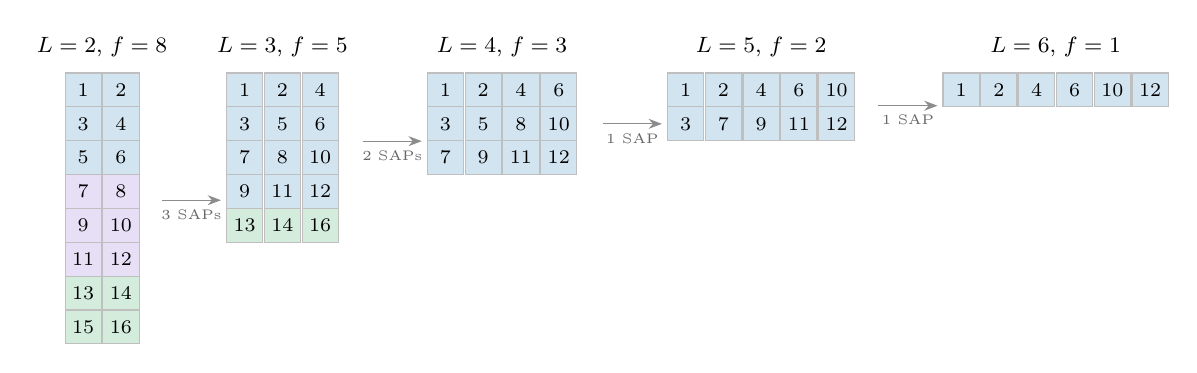
\begin{tikzpicture}[
   cellbox/.style={draw=black!25,minimum width=4.6mm,minimum height=4.3mm,
     inner sep=0pt,font=\scriptsize},
   hd/.style={font=\footnotesize,anchor=south},
   mstep/.style={-{Stealth},black!45},
   steplab/.style={font=\tiny,text=black!60,below}]
\def\w{.48}
\newcommand{\mrow}[4]{% x, y, list, colour
  \foreach \v [count=\i] in {#3}{
    \node[cellbox,fill=#4!35] at ({#1+(\i-1)*\w},{#2}) {\v};}}
\def\h{.43}
% L = 2
\node[hd] at ({0+.5*\w},.3) {$L=2$, $f=8$};
\foreach \a/\b/\c [count=\k from 0] in {1/2/rowA,3/4/rowA,5/6/rowA,7/8/rowB,9/10/rowB,11/12/rowB,13/14/rowC,15/16/rowC}
  {\mrow{0}{-\k*\h}{\a,\b}{\c}}
\draw[mstep] (1.0,-1.4)--(1.75,-1.4) node[steplab,midway] {3 SAPs};
% L = 3
\def\x{2.05}
\node[hd] at ({\x+\w},.3) {$L=3$, $f=5$};
\mrow{\x}{0}{1,2,4}{rowA}
\mrow{\x}{-\h}{3,5,6}{rowA}
\mrow{\x}{-2*\h}{7,8,10}{rowA}
\mrow{\x}{-3*\h}{9,11,12}{rowA}
\mrow{\x}{-4*\h}{13,14,16}{rowC}
\draw[mstep] (3.55,-.65)--(4.3,-.65) node[steplab,midway] {2 SAPs};
% L = 4
\def\x{4.6}
\node[hd] at ({\x+1.5*\w},.3) {$L=4$, $f=3$};
\mrow{\x}{0}{1,2,4,6}{rowA}
\mrow{\x}{-\h}{3,5,8,10}{rowA}
\mrow{\x}{-2*\h}{7,9,11,12}{rowA}
\draw[mstep] (6.6,-.43)--(7.35,-.43) node[steplab,midway] {1 SAP};
% L = 5
\def\x{7.65}
\node[hd] at ({\x+2*\w},.3) {$L=5$, $f=2$};
\mrow{\x}{0}{1,2,4,6,10}{rowA}
\mrow{\x}{-\h}{3,7,9,11,12}{rowA}
\draw[mstep] (10.1,-.2)--(10.85,-.2) node[steplab,midway] {1 SAP};
% L = 6
\def\x{11.15}
\node[hd] at ({\x+2.5*\w},.3) {$L=6$, $f=1$};
\mrow{\x}{0}{1,2,4,6,10,12}{rowA}
\end{tikzpicture}

\caption{The matrices of answer~15(d). Each row is a basic path, given by
the indices of the pairs of the perfect matching that it visits. Within
each matrix, rows of the same colour are merged by one SAP of the next
round (colours are assigned separately in each matrix); the green row at
$L=3$ is itself a SAP, and augmenting along it matches all three of its
pairs by $P$.}
\label{fig:knuth16rows}
\end{figure}

The first matrix says that the matching after~\Hs1 consists of the
couples $b_1g_2$, $b_3g_4$, \dots, $b_{15}g_{16}$. But the graph also
contains the edges $b_5g_8$ and $b_4g_6$, and so this matching has
augmenting paths of two different levels starting at the same free girl
(Fig.~\ref{fig:knuth16paths}):
\begin{equation}
  \pi_2=g_7\sg b_7\db g_8\sg b_8\quad(\text{level }2),\qquad
  \pi_3=g_7\sg b_7\db g_8\sg b_5\db g_6\sg b_4\quad(\text{level }3).
  \label{eq:PQ}
\end{equation}
So the hypothesis of~15(a), that every augmenting path has the same
level, already fails at the first round. On the other hand,
Appendix~\ref{app:knuth16} gives explicit input orders for this graph
under which Algorithm~H follows the schedule $8,5,3,2,1,0$ and passes
through exactly the matrices of Fig.~\ref{fig:knuth16rows}.

\begin{figure}[ht]
\centering
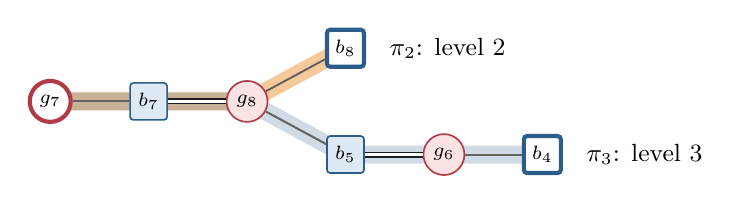
\begin{tikzpicture}[x=1.25cm,y=.9cm]
\node[girl,free] (g7) at (0,0) {$g_7$};
\node[boy] (b7) at (1,0) {$b_7$};
\node[girl] (g8) at (2,0) {$g_8$};
\node[boy,free] (b8) at (3,.75) {$b_8$};
\node[boy] (b5) at (3,-.75) {$b_5$};
\node[girl] (g6) at (4,-.75) {$g_6$};
\node[boy,free] (b4) at (5,-.75) {$b_4$};
\begin{scope}[on background layer]
\draw[sap] (g7.center)--(b7.center)--(g8.center)--(b8.center);
\draw[draw=boydraw,line width=6.5pt,line cap=round,line join=round,opacity=.22]
   (g7.center)--(b7.center)--(g8.center)--(b5.center)--(g6.center)--(b4.center);
\end{scope}
\draw[pedge] (g7)--(b7);
\draw[couple] (b7)--(g8);
\draw[pedge] (g8)--(b8);
\draw[edge,line width=.75pt,draw=black!60] (g8)--(b5);
\draw[couple] (b5)--(g6);
\draw[edge,line width=.75pt,draw=black!60] (g6)--(b4);
\node[font=\small,anchor=west] at (3.35,.75) {$\pi_2$: level 2};
\node[font=\small,anchor=west] at (5.35,-.75) {$\pi_3$: level 3};
\end{tikzpicture}

\caption{Part of Knuth's 16-pair graph after~\Hs1. Both $\pi_2$ (level~2,
three edges) and $\pi_3$ (level~3, five edges) are augmenting paths.}
\label{fig:knuth16paths}
\end{figure}

\subsection{Three readings of the definition}
\label{sec:readings}

Exercise~15(c) calls $G$ a Tchoukaillon graph if it might cause
Algorithm~H ``to continually satisfy assumption (a)'' while following the
schedule. Since the algorithm is deterministic, ``might'' must refer to
the input order of Section~\ref{sec:input}. The example of
Fig.~\ref{fig:knuth16paths} shows that the matrices of answer~15(d)
provide something weaker than assumption~(a). We therefore name three
properties that a round with $f$ free girls at level~$L$ may have:
\begin{itemize}
\item[$\Up$:] every augmenting path has level~$L$ (the literal hypothesis
  of 15(a); $\Up$ for ``uniform'');
\item[$\Bp$:] there are $f$ vertex-disjoint SAPs, that is, $\nu=f$;
  equivalently, for some perfect matching all $f$ basic paths are SAPs
  (what the matrices show; $\Bp$ for ``full'');
\item[$\Op$:] no condition beyond the numbers.
\end{itemize}

\begin{definition}
An ordered graph with a perfect matching \emph{realizes the Tchoukaillon
schedule} if~\Hs1 leaves $\floor{s/2}$ free girls and every later round
has the level~$L$ and the number of SAPs $a_L$ prescribed by
\eqref{eq:schedule}. A realization is \emph{literal} if every round after
\Hs1 has property~$\Up$, and \emph{basic-row} if every such round has
property~$\Bp$. We call a realization with no extra condition
\emph{operational}.
\end{definition}

Property $\Up$ implies $\Bp$, since the basic paths are augmenting paths.
Property $\Bp$ is exactly what Lemma~\ref{lem:15ab}(b) needs to force
$\ceil{f/(L+1)}$ SAPs. Neither implication reverses: Knuth's graph is a
basic-row realization that is not literal, and Section~\ref{sec:no-cover}
gives an operational realization (an 8-pair tree) in which a round has
two free girls but only one SAP, so it is not basic-row.

Which reading did Knuth intend? The literal one is what 15(a) and 15(c)
say. The matrices of 15(d) support the basic-row reading, and the
motivation---making Algorithm~H slow---supports the operational one;
the abstract of Knuth's 2022 lecture on Tchoukaillon numbers
\cite{KnuthRutgers} poses the matching question in terms of running
time. These notes do not choose. They answer the literal question
completely (Section~\ref{sec:literal}), and report partial results on the
other two (Section~\ref{sec:operational}).

Finally there is the question raised in the answer to exercise~16:
whether some graph forces \emph{more} rounds than a Tchoukaillon graph
would, ``by violating assumption~(a) and/or by finding more SAPs.'' Here
no condition is imposed on the run at all. Let
\[
  R(s)=\max\ \{\,\text{number of rounds of Algorithm~H}\,\},
\]
the maximum over all ordered bipartite graphs whose maximum matching has
size~$s$. (Neither a perfect matching nor any particular initial
matching is required.) Sections~\ref{sec:upper}--\ref{sec:comparison}
determine $R(s)$ exactly. Table~\ref{tab:readings} summarizes the
four questions and what these notes establish about them.

\begin{table}[ht]
\centering\small
\begin{tabular}{>{\raggedright\arraybackslash}p{.2\textwidth}
  >{\raggedright\arraybackslash}p{.34\textwidth}
  >{\raggedright\arraybackslash}p{.36\textwidth}}
\toprule
Question & Requirement & Answer here\\
\midrule
Literal & schedule, and $\Up$ in every round & for $s\ge1$, exists
  exactly when $s\in\{1,2,3,4,5,8,9\}$ (Corollary~L)\\[3pt]
Basic-row & schedule, and $\Bp$ in every round & explicit inputs for all
  $s\le57$ (Appendix~\ref{app:catalog}), including Knuth's graph; open in
  general\\[3pt]
Operational & schedule only & the same inputs; open in general; necessary
  conditions in Section~\ref{sec:operational}\\[3pt]
Most rounds & nothing & $R(s)=\floor{\sqrt{4s+1}}-1$ (Theorem~R);
  always $R(s)\ge T(s)$, with strict inequality first at $s=9$ and for
  all large $s$ (Section~\ref{sec:comparison})\\
\bottomrule
\end{tabular}
\caption{Four questions suggested by exercises~15 and 16.}
\label{tab:readings}
\end{table}

\section{How many rounds can there be?}
\label{sec:upper}

Here is the main theorem. Recall that rounds are counted with~\Hs1 as
the first one (Section~\ref{sec:counting}), and let
\[
   Q_n=\bigfloor{\frac{(n+1)^2}{4}}=\bigfloor{\frac{n+1}2}\bigceil{\frac{n+1}2},
\]
the quarter-squares $(Q_1,Q_2,Q_3,\ldots)=(1,2,4,6,9,12,16,20,25,30,36,42,\ldots)$.

\begin{lthm}{R}
Let $s\ge0$. Every ordered bipartite graph whose maximum matching has
size~$s$ makes Algorithm~H perform at most
\[
   R(s)=\bigfloor{\sqrt{4s+1}}-1
\]
rounds, and some ordered graph with $M=N=s$ attains this number.
Equivalently, $n$ rounds are possible if and only if $s\ge Q_n$.
\end{lthm}

The two formulations agree: $Q_n\le s$ means $(n+1)^2<4s+4$, that is
$(n+1)^2\le4s+3$; since squares are $0$ or $1$ modulo~$4$, this is the
same as $(n+1)^2\le4s+1$, or $n\le\floor{\sqrt{4s+1}}-1$.

This section proves the upper bound. Section~\ref{sec:staircase}
constructs graphs that attain it.

\subsection{A rectangle that must fit}

The argument is the one in the proof of Theorem~H, applied at the start
of a round instead of at the end.

\begin{lemma}
\label{lem:rectangle}
Suppose that before some round the current matching has $s'$ couples,
and that its shortest augmenting paths have level~$L$. Then
\[
   (s-s')\,L\ \le\ s .
\]
\end{lemma}

\begin{proof}
The union of the current matching with a maximum matching contains
$s-s'$ vertex-disjoint augmenting paths. Each has level at least $L$,
hence contains at least $L$ edges of the maximum matching. These edges
are distinct, and there are only $s$ of them.
\end{proof}

When $s=M=N$, the deficiency $s-s'$ is the number $f$ of free girls, and
the lemma says that the $f$ basic paths, drawn as rows of at least~$L$
cells each, contain an $f\times L$ rectangle inside the set of all $s$
cells (Fig.~\ref{fig:hyperbola}, left). Nothing requires the rows to have
equal numbers of cells; a basic path may have a much higher level than a
SAP.

\begin{figure}[ht]
\centering
% Left: basic paths as rows (s = 20); right: the (L,f) plane for s = 16.
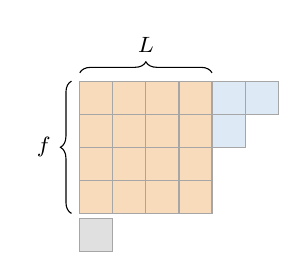
\begin{tikzpicture}[x=.42cm,y=.42cm,baseline=(current bounding box.center)]
  % rows of 6,5,4,4 cells (= 19 cells) plus one cell on no basic path
  \foreach \len [count=\r] in {6,5,4,4}{
    \foreach \c in {1,...,\len}{
      \ifnum\c<5
        \draw[fill=sapcol!30,draw=black!35] (\c-1,-\r) rectangle (\c,-\r+1);
      \else
        \draw[fill=boyfill,draw=black!35] (\c-1,-\r) rectangle (\c,-\r+1);
      \fi}}
  \draw[fill=black!12,draw=black!35] (0,-5.15) rectangle (1,-4.15);
  \draw[decorate,decoration={brace,amplitude=4pt}] (-.25,-4)--(-.25,0)
    node[midway,left=4pt,font=\footnotesize] {$f$};
  \draw[decorate,decoration={brace,amplitude=4pt}] (0,.25)--(4,.25)
    node[midway,above=4pt,font=\footnotesize] {$L$};
\end{tikzpicture}\hspace{12mm}%
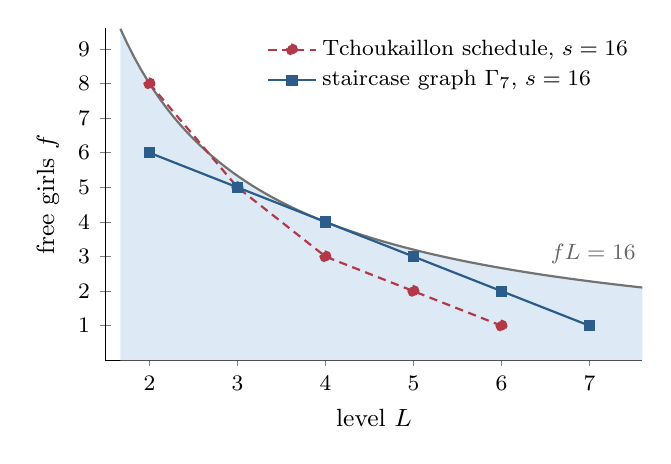
\begin{tikzpicture}[baseline=(current bounding box.center)]
\begin{axis}[
  width=8.4cm,height=5.8cm, xmin=1.5,xmax=7.6,ymin=0,ymax=9.6,
  xtick={2,...,7},ytick={1,...,9},
  xlabel={level $L$}, ylabel={free girls $f$},
  axis lines=left, axis line style={-}, tick label style={font=\footnotesize},
  label style={font=\small},
  legend style={draw=none,fill=none,at={(1.0,1.0)},anchor=north east,font=\footnotesize,
    cells={anchor=west}}]
  \addplot[forget plot,fill=boyfill,draw=none,domain=1.67:7.6,samples=80] {16/x} \closedcycle;
  \addplot[forget plot,domain=1.67:7.6,samples=80,black!55,thick] {16/x};
  \addplot[chcol,mark=*,mark size=1.8pt,thick,densely dashed]
     coordinates {(2,8) (3,5) (4,3) (5,2) (6,1)};
  \addlegendentry{Tchoukaillon schedule, $s=16$}
  \addplot[qcol,mark=square*,mark size=1.6pt,thick]
     coordinates {(2,6) (3,5) (4,4) (5,3) (6,2) (7,1)};
  \addlegendentry{staircase graph $\Gamma_7$, $s=16$}
  \node[font=\footnotesize,black!60,anchor=south west] at (axis cs:6.45,2.5) {$fL=16$};
\end{axis}
\end{tikzpicture}

\caption{Left: an example with $s=20$ and $f=4$. The basic paths of the
matching are drawn one per row, each with at least $L=4$ cells (one cell
per pair of the perfect matching); the grey cell lies on no basic path.
The shaded $f\times L$ rectangle shows why $fL\le s$. Right: every round
of every run is a point $(L,f)$ on or below the hyperbola $fL=s$. Both
trajectories shown take $s=16$; the staircase graph of
Section~\ref{sec:staircase} starts with fewer free girls but loses only
one per round, and so lasts longer.}
\label{fig:hyperbola}
\end{figure}

\subsection{Proof of the upper bound}

Suppose a run has $n\ge2$ rounds, so that there are $n-1$ successful
rounds after~\Hs1. Number these $i=1,2,\ldots,n-1$ and let round~$i$
have level~$L_i$ and start with deficiency $d_i=s-s'$.

\begin{itemize}
\item $L_i\ge i+1$. Indeed $L_1\ge2$ because the matching produced by~\Hs1 is
maximal, and the levels strictly increase from round to round.
\item $d_i\ge n-i$. Indeed each of the rounds~$i,i+1,\ldots,n-1$ adds at
least one couple.
\end{itemize}
By Lemma~\ref{lem:rectangle}, $s\ge(i+1)(n-i)$ for every $i$. The two
factors add up to $n+1$, so the product is largest when they are as
nearly equal as possible: taking $i+1=\ceil{(n+1)/2}$ gives
$s\ge\floor{(n+1)/2}\ceil{(n+1)/2}=Q_n$. A run with a single round needs
an edge, so $s\ge1=Q_1$. This proves the upper bound in Theorem~R.
\qed

\medskip
Hopcroft and Karp bounded the number of distinct path lengths, and
hence the number of phases, by $2\floor{\sqrt s}+2$ \cite[Theorem~3]{HK},
by essentially this argument applied at a single well-chosen phase.
Using it at every round gives the exact threshold~$Q_n$. What is new in
Theorem~R is that this threshold is attained.

\subsection{What a run with the most rounds must look like}
\label{sec:equality}

If $s=Q_n$ and a run has $n$ rounds, then the inequalities in the proof
are tight at a middle round~$i$, where $(i+1)(n-i)=Q_n$. That round has
level exactly $L=i+1$ and deficiency exactly $f=n-i$, and the $f$
disjoint augmenting paths supplied by a maximum matching are all SAPs,
which together use every one of its $s$ edges. So $\nu=f$ there, and in
the picture the $f\times L$ rectangle fills all $s$ cells, as in Knuth's
matrices. From that round on, every round removes exactly one SAP.

The rounds before the middle are where a worst case can differ from a
Tchoukaillon graph. There $f$ can exceed $L+1$, and then, if $\nu$ were
equal to $f$, Lemma~\ref{lem:15ab}(b) would force at least two SAPs in the
round. The
staircase graphs of Section~\ref{sec:staircase} avoid this by making some
basic paths longer than~$L$: those paths are counted in~$f$ but are not
SAPs, so $\nu\le L+1$ and a single SAP can meet all the shortest ones.
Fig.~\ref{fig:hyperbola} (right) shows the effect: the Tchoukaillon
schedule starts at the top of the hyperbola and must shed free girls
quickly, while the staircase graph starts lower and slides down along it,
one free girl per round.

\section{Staircase graphs}
\label{sec:staircase}

This section constructs, for every $n\ge2$, an ordered graph $\Gam_n$
with $s=Q_n$ on which Algorithm~H performs $n$ rounds, and proves exactly
what the algorithm does on it. The graph of Fig.~\ref{fig:gamma5} is
$\Gam_5$. The idea, already visible in Section~\ref{sec:worked}, is to let
the basic paths have different levels, and to arrange the input so that
the depth-first search always finds one SAP that crosses every shortest
basic path. That single path blocks all the others.

\subsection{The graph and its input}
\label{sec:gamma}

Fix $n\ge2$. The graph $\Gam_n$ is built on a diagram of \emph{cells}
arranged in $n-1$ left-justified rows. Row~$a$ has
\[
   \ell_a=\max\Bigl(2,\ \bigfloor{\frac{n+2-a}{2}}\Bigr)\qquad(1\le a\le n-1)
\]
cells, so the numbers of cells decrease by one every two rows, except that the
last row has two cells. Equivalently, cell~$(a,c)$ (row~$a$, column~$c$)
exists if $a+2c\le n+2$, and there is one more cell~$(n-1,2)$, which we
call the \emph{corner}. For $n=5$ the rows have $3,2,2,2$ cells; for
$n=11$ they are $6,5,5,4,4,3,3,2,2,2$ (Fig.~\ref{fig:shape}).

\begin{figure}[ht]
\centering
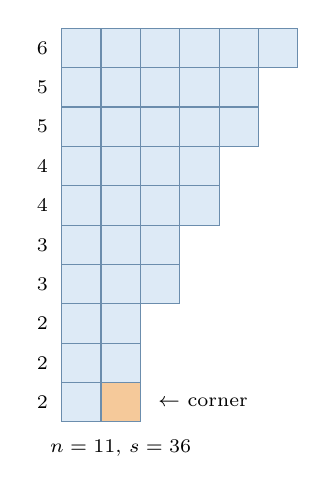
\begin{tikzpicture}[]
\draw[fill=boyfill,draw=boydraw!70] (0.00,0.00) rectangle +(0.50,0.50);
\draw[fill=boyfill,draw=boydraw!70] (0.50,0.00) rectangle +(0.50,0.50);
\draw[fill=boyfill,draw=boydraw!70] (1.00,0.00) rectangle +(0.50,0.50);
\draw[fill=boyfill,draw=boydraw!70] (1.50,0.00) rectangle +(0.50,0.50);
\draw[fill=boyfill,draw=boydraw!70] (2.00,0.00) rectangle +(0.50,0.50);
\draw[fill=boyfill,draw=boydraw!70] (2.50,0.00) rectangle +(0.50,0.50);
\node[font=\scriptsize,anchor=east] at (-.05,0.25) {6};
\draw[fill=boyfill,draw=boydraw!70] (0.00,-0.50) rectangle +(0.50,0.50);
\draw[fill=boyfill,draw=boydraw!70] (0.50,-0.50) rectangle +(0.50,0.50);
\draw[fill=boyfill,draw=boydraw!70] (1.00,-0.50) rectangle +(0.50,0.50);
\draw[fill=boyfill,draw=boydraw!70] (1.50,-0.50) rectangle +(0.50,0.50);
\draw[fill=boyfill,draw=boydraw!70] (2.00,-0.50) rectangle +(0.50,0.50);
\node[font=\scriptsize,anchor=east] at (-.05,-0.25) {5};
\draw[fill=boyfill,draw=boydraw!70] (0.00,-1.00) rectangle +(0.50,0.50);
\draw[fill=boyfill,draw=boydraw!70] (0.50,-1.00) rectangle +(0.50,0.50);
\draw[fill=boyfill,draw=boydraw!70] (1.00,-1.00) rectangle +(0.50,0.50);
\draw[fill=boyfill,draw=boydraw!70] (1.50,-1.00) rectangle +(0.50,0.50);
\draw[fill=boyfill,draw=boydraw!70] (2.00,-1.00) rectangle +(0.50,0.50);
\node[font=\scriptsize,anchor=east] at (-.05,-0.75) {5};
\draw[fill=boyfill,draw=boydraw!70] (0.00,-1.50) rectangle +(0.50,0.50);
\draw[fill=boyfill,draw=boydraw!70] (0.50,-1.50) rectangle +(0.50,0.50);
\draw[fill=boyfill,draw=boydraw!70] (1.00,-1.50) rectangle +(0.50,0.50);
\draw[fill=boyfill,draw=boydraw!70] (1.50,-1.50) rectangle +(0.50,0.50);
\node[font=\scriptsize,anchor=east] at (-.05,-1.25) {4};
\draw[fill=boyfill,draw=boydraw!70] (0.00,-2.00) rectangle +(0.50,0.50);
\draw[fill=boyfill,draw=boydraw!70] (0.50,-2.00) rectangle +(0.50,0.50);
\draw[fill=boyfill,draw=boydraw!70] (1.00,-2.00) rectangle +(0.50,0.50);
\draw[fill=boyfill,draw=boydraw!70] (1.50,-2.00) rectangle +(0.50,0.50);
\node[font=\scriptsize,anchor=east] at (-.05,-1.75) {4};
\draw[fill=boyfill,draw=boydraw!70] (0.00,-2.50) rectangle +(0.50,0.50);
\draw[fill=boyfill,draw=boydraw!70] (0.50,-2.50) rectangle +(0.50,0.50);
\draw[fill=boyfill,draw=boydraw!70] (1.00,-2.50) rectangle +(0.50,0.50);
\node[font=\scriptsize,anchor=east] at (-.05,-2.25) {3};
\draw[fill=boyfill,draw=boydraw!70] (0.00,-3.00) rectangle +(0.50,0.50);
\draw[fill=boyfill,draw=boydraw!70] (0.50,-3.00) rectangle +(0.50,0.50);
\draw[fill=boyfill,draw=boydraw!70] (1.00,-3.00) rectangle +(0.50,0.50);
\node[font=\scriptsize,anchor=east] at (-.05,-2.75) {3};
\draw[fill=boyfill,draw=boydraw!70] (0.00,-3.50) rectangle +(0.50,0.50);
\draw[fill=boyfill,draw=boydraw!70] (0.50,-3.50) rectangle +(0.50,0.50);
\node[font=\scriptsize,anchor=east] at (-.05,-3.25) {2};
\draw[fill=boyfill,draw=boydraw!70] (0.00,-4.00) rectangle +(0.50,0.50);
\draw[fill=boyfill,draw=boydraw!70] (0.50,-4.00) rectangle +(0.50,0.50);
\node[font=\scriptsize,anchor=east] at (-.05,-3.75) {2};
\draw[fill=boyfill,draw=boydraw!70] (0.00,-4.50) rectangle +(0.50,0.50);
\draw[fill=sapcol!45,draw=boydraw!70] (0.50,-4.50) rectangle +(0.50,0.50);
\node[font=\scriptsize,anchor=east] at (-.05,-4.25) {2};
\node[font=\scriptsize,anchor=west] at (1.10,-4.25) {$\leftarrow$ corner};
\node[font=\scriptsize,anchor=north] at (0.75,-4.60) {$n=11$, $s=36$};
\end{tikzpicture}

\caption{The cell diagram of $\Gam_{11}$; the numbers on the left are the
numbers of cells in the rows. The shaded cell is the corner cell~$(10,2)$.}
\label{fig:shape}
\end{figure}

Each cell~$(a,c)$ holds a girl~$g_{a,c}$ and a boy~$b_{a,c}$. The edges are
\begin{itemize}
\item $g_{a,c}\sg b_{a,c}$ for every cell (the \emph{inside} edges);
\item $b_{a,c}\sg g_{a,c+1}$ whenever both cells exist (\emph{horizontal}
  edges, from a boy to the girl of the next cell in his row);
\item $b_{a,c}\sg g_{a+1,c}$ whenever both cells exist (\emph{vertical}
  edges, from a boy to the girl of the cell below), \emph{except} the
  single edge $b_{n-2,2}\sg g_{n-1,2}$ into the corner, which is omitted.
\end{itemize}
The omission is a convenience for the proofs. With that edge present,
Algorithm~H still performs $n$ rounds of one SAP each (we have checked
this for $n\le30$), but in every round with at least two free girls the
corner girl would join the list $\A{BLINK}$ of a free boy, which breaks
the clean description in Lemma~\ref{lem:bfs} and changes the counts of
Theorem~W.
So a girl is adjacent to at most three boys: the boy to her left, the boy
above her, and her own. In Fig.~\ref{fig:gamma5} girls sit at the
upper left of their cells and boys at the lower right, so horizontal
edges run up and to the right, and vertical edges down and to the left.

\paragraph{The input order.}
Number the boys~$1,2,\ldots,s$ in row-major order of their cells (row by
row, left to right). Number the first girl of each row, $g_{a,1}$, as
$n-a$; number the remaining girls~$n,n+1,\ldots,s$ in row-major order.
Each girl's list consists of
\[
  \text{her left boy } b_{a,c-1},\quad\text{then her upper boy } b_{a-1,c},
  \quad\text{then her own boy } b_{a,c},
\]
omitting those that do not exist or are not adjacent to her. For $n=5$
this gives the lists~\eqref{eq:gamma5lists}.

\begin{proposition}
\label{prop:gamma}
The graph $\Gam_n$ is connected and planar, and has maximum degree three.
Its inside edges form a perfect matching, and
\[
   M=N=s=Q_n,\qquad E=3Q_n-n-\bigfloor{\frac{n+1}2}.
\]
Step~\Hs1 couples every horizontal edge $b_{a,c}\db g_{a,c+1}$. It leaves
free exactly the first girl and the last boy of every row, and puts the
free girls into \A{QUEUE} in row order~$g_{1,1},g_{2,1},\ldots,g_{n-1,1}$.
It examines $s+n-2$ adjacency entries.
\end{proposition}

\begin{proof}
Substituting $j=n+2-a$, the numbers of cells in the rows are $\max(2,\floor{j/2})$ for
$3\le j\le n+1$. Since $\sum_{j=1}^{m}\floor{j/2}=\floor{m^2/4}$, their sum is
$\floor{(n+1)^2/4}-\floor{1/2}-\floor{2/2}+1=Q_n$. There are $s$ inside
edges, $s-(n-1)$ horizontal edges, and one vertical edge into every cell
outside row~1 except the corner, so $s-\ell_1-1$ vertical edges when
$n\ge3$; with $\ell_1=\floor{(n+1)/2}$ this gives $E$ (and $n=2$ is
checked directly). Girls have at most three neighbors by construction,
and so do boys (their own girl, the girl to the right, and the girl
below). Rows are connected by their horizontal and inside edges, and the
vertical edges in column~1 connect the rows. The drawing of
Fig.~\ref{fig:gamma5} has no crossings, because every edge stays inside
its own cell or in the gap between two adjacent cells.

Step~\Hs1 scans girls~$s,s-1,\ldots,n$ first; these are the girls not in
column~1, and each takes the first boy on her list, her left boy. All
these boys are different. Then girls~$n-1,\ldots,1$, the first girls of
rows~$1,\ldots,n-1$, find their upper and own boys taken. The count of
examinations is $(s-n+1)+1+2(n-2)$.
\end{proof}

\subsection{Watching the smallest interesting case}
\label{sec:watch}

Before the general proof, look at the whole run on $\Gam_5$
(Fig.~\ref{fig:gamma5rounds}). The coloured bands are the basic paths
relative to the inside-edge perfect matching. Initially they are the rows
of the diagram, with $3,2,2,2$ cells, that is, of levels~$3,2,2,2$. The
three basic paths of level~2 are disjoint SAPs, so the dag has $L=2$ and
$\nu=3$, while $f=4$. Yet the single SAP that Algorithm~H finds runs from
the free girl of row~4 up through row~3 to the free boy of row~2, meeting
all three. After augmenting there are three basic paths, each with three
cells: the full rectangle that Section~\ref{sec:equality} demands. The
next SAP climbs a staircase through all three of them, and so on.

\begin{figure}[ht]
\centering
\resizebox{\linewidth}{!}{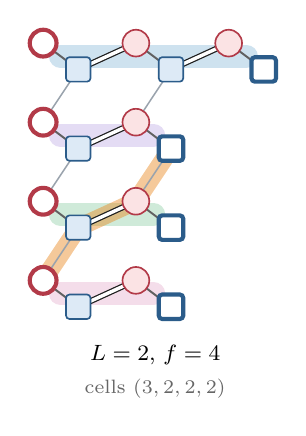
\begin{tikzpicture}[baseline=(current bounding box.north)]
\begin{scope}[on background layer]
\draw[hook,rowA] (0.000,0.000) -- (1.178,0.000) -- (2.356,0.000);
\draw[hook,rowB] (0.000,-1.004) -- (1.178,-1.004);
\draw[hook,rowC] (0.000,-2.009) -- (1.178,-2.009);
\draw[hook,rowD] (0.000,-3.013) -- (1.178,-3.013);
\draw[sap] (-0.223,-2.846) -- (0.223,-2.176) -- (0.955,-1.841) -- (1.401,-1.172);
\end{scope}
\draw[edge] (-0.223,-2.846) -- (0.223,-2.176);
\draw[pedge] (-0.223,-2.846) -- (0.223,-3.181);
\draw[edge] (-0.223,-1.841) -- (0.223,-1.172);
\draw[pedge] (-0.223,-1.841) -- (0.223,-2.176);
\draw[edge] (-0.223,-0.837) -- (0.223,-0.167);
\draw[pedge] (-0.223,-0.837) -- (0.223,-1.172);
\draw[pedge] (-0.223,0.167) -- (0.223,-0.167);
\draw[couple] (0.955,0.167) -- (0.223,-0.167);
\draw[pedge] (0.955,0.167) -- (1.401,-0.167);
\draw[couple] (2.133,0.167) -- (1.401,-0.167);
\draw[pedge] (2.133,0.167) -- (2.579,-0.167);
\draw[couple] (0.955,-0.837) -- (0.223,-1.172);
\draw[edge] (0.955,-0.837) -- (1.401,-0.167);
\draw[pedge] (0.955,-0.837) -- (1.401,-1.172);
\draw[couple] (0.955,-1.841) -- (0.223,-2.176);
\draw[edge] (0.955,-1.841) -- (1.401,-1.172);
\draw[pedge] (0.955,-1.841) -- (1.401,-2.176);
\draw[couple] (0.955,-2.846) -- (0.223,-3.181);
\draw[pedge] (0.955,-2.846) -- (1.401,-3.181);
\node[small girl,free] at (-0.223,-2.846) {};
\node[small girl,free] at (-0.223,-1.841) {};
\node[small girl,free] at (-0.223,-0.837) {};
\node[small girl,free] at (-0.223,0.167) {};
\node[small girl] at (0.955,0.167) {};
\node[small girl] at (2.133,0.167) {};
\node[small girl] at (0.955,-0.837) {};
\node[small girl] at (0.955,-1.841) {};
\node[small girl] at (0.955,-2.846) {};
\node[small boy] at (0.223,-0.167) {};
\node[small boy] at (1.401,-0.167) {};
\node[small boy,free] at (2.579,-0.167) {};
\node[small boy] at (0.223,-1.172) {};
\node[small boy,free] at (1.401,-1.172) {};
\node[small boy] at (0.223,-2.176) {};
\node[small boy,free] at (1.401,-2.176) {};
\node[small boy] at (0.223,-3.181) {};
\node[small boy,free] at (1.401,-3.181) {};
\node[font=\footnotesize,anchor=north] at (1.2,-3.55) {$L=2$, $f=4$};
\node[font=\scriptsize,text=black!60,anchor=north] at (1.2,-3.98) {cells $(3,2,2,2)$};
\end{tikzpicture}
\hspace{7mm}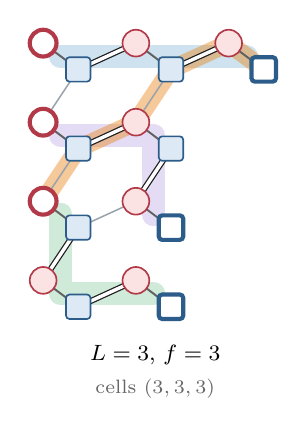
\begin{tikzpicture}[baseline=(current bounding box.north)]
\begin{scope}[on background layer]
\draw[hook,rowA] (0.000,0.000) -- (1.178,0.000) -- (2.356,0.000);
\draw[hook,rowB] (0.000,-1.004) -- (1.178,-1.004) -- (1.178,-2.009);
\draw[hook,rowC] (0.000,-2.009) -- (0.000,-3.013) -- (1.178,-3.013);
\draw[sap] (-0.223,-1.841) -- (0.223,-1.172) -- (0.955,-0.837) -- (1.401,-0.167) -- (2.133,0.167) -- (2.579,-0.167);
\end{scope}
\draw[couple] (-0.223,-2.846) -- (0.223,-2.176);
\draw[pedge] (-0.223,-2.846) -- (0.223,-3.181);
\draw[edge] (-0.223,-1.841) -- (0.223,-1.172);
\draw[pedge] (-0.223,-1.841) -- (0.223,-2.176);
\draw[edge] (-0.223,-0.837) -- (0.223,-0.167);
\draw[pedge] (-0.223,-0.837) -- (0.223,-1.172);
\draw[pedge] (-0.223,0.167) -- (0.223,-0.167);
\draw[couple] (0.955,0.167) -- (0.223,-0.167);
\draw[pedge] (0.955,0.167) -- (1.401,-0.167);
\draw[couple] (2.133,0.167) -- (1.401,-0.167);
\draw[pedge] (2.133,0.167) -- (2.579,-0.167);
\draw[couple] (0.955,-0.837) -- (0.223,-1.172);
\draw[edge] (0.955,-0.837) -- (1.401,-0.167);
\draw[pedge] (0.955,-0.837) -- (1.401,-1.172);
\draw[edge] (0.955,-1.841) -- (0.223,-2.176);
\draw[couple] (0.955,-1.841) -- (1.401,-1.172);
\draw[pedge] (0.955,-1.841) -- (1.401,-2.176);
\draw[couple] (0.955,-2.846) -- (0.223,-3.181);
\draw[pedge] (0.955,-2.846) -- (1.401,-3.181);
\node[small girl] at (-0.223,-2.846) {};
\node[small girl,free] at (-0.223,-1.841) {};
\node[small girl,free] at (-0.223,-0.837) {};
\node[small girl,free] at (-0.223,0.167) {};
\node[small girl] at (0.955,0.167) {};
\node[small girl] at (2.133,0.167) {};
\node[small girl] at (0.955,-0.837) {};
\node[small girl] at (0.955,-1.841) {};
\node[small girl] at (0.955,-2.846) {};
\node[small boy] at (0.223,-0.167) {};
\node[small boy] at (1.401,-0.167) {};
\node[small boy,free] at (2.579,-0.167) {};
\node[small boy] at (0.223,-1.172) {};
\node[small boy] at (1.401,-1.172) {};
\node[small boy] at (0.223,-2.176) {};
\node[small boy,free] at (1.401,-2.176) {};
\node[small boy] at (0.223,-3.181) {};
\node[small boy,free] at (1.401,-3.181) {};
\node[font=\footnotesize,anchor=north] at (1.2,-3.55) {$L=3$, $f=3$};
\node[font=\scriptsize,text=black!60,anchor=north] at (1.2,-3.98) {cells $(3,3,3)$};
\end{tikzpicture}
\hspace{7mm}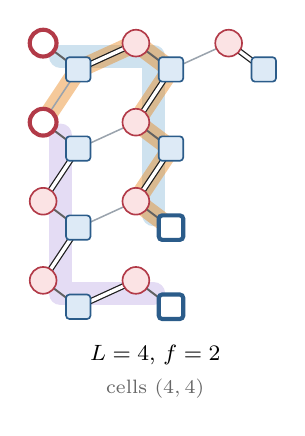
\begin{tikzpicture}[baseline=(current bounding box.north)]
\begin{scope}[on background layer]
\draw[hook,rowA] (0.000,0.000) -- (1.178,0.000) -- (1.178,-1.004) -- (1.178,-2.009);
\draw[hook,rowB] (0.000,-1.004) -- (0.000,-2.009) -- (0.000,-3.013) -- (1.178,-3.013);
\draw[sap] (-0.223,-0.837) -- (0.223,-0.167) -- (0.955,0.167) -- (1.401,-0.167) -- (0.955,-0.837) -- (1.401,-1.172) -- (0.955,-1.841) -- (1.401,-2.176);
\end{scope}
\draw[couple] (-0.223,-2.846) -- (0.223,-2.176);
\draw[pedge] (-0.223,-2.846) -- (0.223,-3.181);
\draw[couple] (-0.223,-1.841) -- (0.223,-1.172);
\draw[pedge] (-0.223,-1.841) -- (0.223,-2.176);
\draw[edge] (-0.223,-0.837) -- (0.223,-0.167);
\draw[pedge] (-0.223,-0.837) -- (0.223,-1.172);
\draw[pedge] (-0.223,0.167) -- (0.223,-0.167);
\draw[couple] (0.955,0.167) -- (0.223,-0.167);
\draw[pedge] (0.955,0.167) -- (1.401,-0.167);
\draw[edge] (2.133,0.167) -- (1.401,-0.167);
\draw[couple] (2.133,0.167) -- (2.579,-0.167);
\draw[edge] (0.955,-0.837) -- (0.223,-1.172);
\draw[couple] (0.955,-0.837) -- (1.401,-0.167);
\draw[pedge] (0.955,-0.837) -- (1.401,-1.172);
\draw[edge] (0.955,-1.841) -- (0.223,-2.176);
\draw[couple] (0.955,-1.841) -- (1.401,-1.172);
\draw[pedge] (0.955,-1.841) -- (1.401,-2.176);
\draw[couple] (0.955,-2.846) -- (0.223,-3.181);
\draw[pedge] (0.955,-2.846) -- (1.401,-3.181);
\node[small girl] at (-0.223,-2.846) {};
\node[small girl] at (-0.223,-1.841) {};
\node[small girl,free] at (-0.223,-0.837) {};
\node[small girl,free] at (-0.223,0.167) {};
\node[small girl] at (0.955,0.167) {};
\node[small girl] at (2.133,0.167) {};
\node[small girl] at (0.955,-0.837) {};
\node[small girl] at (0.955,-1.841) {};
\node[small girl] at (0.955,-2.846) {};
\node[small boy] at (0.223,-0.167) {};
\node[small boy] at (1.401,-0.167) {};
\node[small boy] at (2.579,-0.167) {};
\node[small boy] at (0.223,-1.172) {};
\node[small boy] at (1.401,-1.172) {};
\node[small boy] at (0.223,-2.176) {};
\node[small boy,free] at (1.401,-2.176) {};
\node[small boy] at (0.223,-3.181) {};
\node[small boy,free] at (1.401,-3.181) {};
\node[font=\footnotesize,anchor=north] at (1.2,-3.55) {$L=4$, $f=2$};
\node[font=\scriptsize,text=black!60,anchor=north] at (1.2,-3.98) {cells $(4,4)$};
\end{tikzpicture}
\hspace{7mm}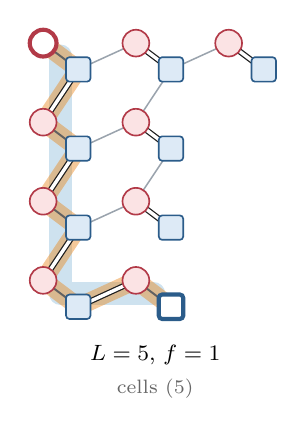
\begin{tikzpicture}[baseline=(current bounding box.north)]
\begin{scope}[on background layer]
\draw[hook,rowA] (0.000,0.000) -- (0.000,-1.004) -- (0.000,-2.009) -- (0.000,-3.013) -- (1.178,-3.013);
\draw[sap] (-0.223,0.167) -- (0.223,-0.167) -- (-0.223,-0.837) -- (0.223,-1.172) -- (-0.223,-1.841) -- (0.223,-2.176) -- (-0.223,-2.846) -- (0.223,-3.181) -- (0.955,-2.846) -- (1.401,-3.181);
\end{scope}
\draw[couple] (-0.223,-2.846) -- (0.223,-2.176);
\draw[pedge] (-0.223,-2.846) -- (0.223,-3.181);
\draw[couple] (-0.223,-1.841) -- (0.223,-1.172);
\draw[pedge] (-0.223,-1.841) -- (0.223,-2.176);
\draw[couple] (-0.223,-0.837) -- (0.223,-0.167);
\draw[pedge] (-0.223,-0.837) -- (0.223,-1.172);
\draw[pedge] (-0.223,0.167) -- (0.223,-0.167);
\draw[edge] (0.955,0.167) -- (0.223,-0.167);
\draw[couple] (0.955,0.167) -- (1.401,-0.167);
\draw[edge] (2.133,0.167) -- (1.401,-0.167);
\draw[couple] (2.133,0.167) -- (2.579,-0.167);
\draw[edge] (0.955,-0.837) -- (0.223,-1.172);
\draw[edge] (0.955,-0.837) -- (1.401,-0.167);
\draw[couple] (0.955,-0.837) -- (1.401,-1.172);
\draw[edge] (0.955,-1.841) -- (0.223,-2.176);
\draw[edge] (0.955,-1.841) -- (1.401,-1.172);
\draw[couple] (0.955,-1.841) -- (1.401,-2.176);
\draw[couple] (0.955,-2.846) -- (0.223,-3.181);
\draw[pedge] (0.955,-2.846) -- (1.401,-3.181);
\node[small girl] at (-0.223,-2.846) {};
\node[small girl] at (-0.223,-1.841) {};
\node[small girl] at (-0.223,-0.837) {};
\node[small girl,free] at (-0.223,0.167) {};
\node[small girl] at (0.955,0.167) {};
\node[small girl] at (2.133,0.167) {};
\node[small girl] at (0.955,-0.837) {};
\node[small girl] at (0.955,-1.841) {};
\node[small girl] at (0.955,-2.846) {};
\node[small boy] at (0.223,-0.167) {};
\node[small boy] at (1.401,-0.167) {};
\node[small boy] at (2.579,-0.167) {};
\node[small boy] at (0.223,-1.172) {};
\node[small boy] at (1.401,-1.172) {};
\node[small boy] at (0.223,-2.176) {};
\node[small boy] at (1.401,-2.176) {};
\node[small boy] at (0.223,-3.181) {};
\node[small boy,free] at (1.401,-3.181) {};
\node[font=\footnotesize,anchor=north] at (1.2,-3.55) {$L=5$, $f=1$};
\node[font=\scriptsize,text=black!60,anchor=north] at (1.2,-3.98) {cells $(5)$};
\end{tikzpicture}
\hspace{7mm}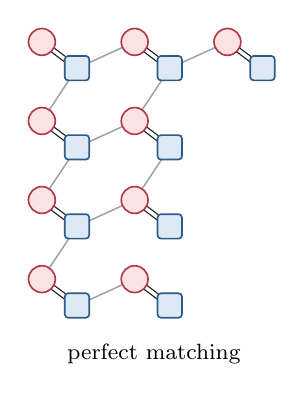
\begin{tikzpicture}[baseline=(current bounding box.north)]
\begin{scope}[on background layer]
\end{scope}
\draw[edge] (-0.223,-2.846) -- (0.223,-2.176);
\draw[couple] (-0.223,-2.846) -- (0.223,-3.181);
\draw[edge] (-0.223,-1.841) -- (0.223,-1.172);
\draw[couple] (-0.223,-1.841) -- (0.223,-2.176);
\draw[edge] (-0.223,-0.837) -- (0.223,-0.167);
\draw[couple] (-0.223,-0.837) -- (0.223,-1.172);
\draw[couple] (-0.223,0.167) -- (0.223,-0.167);
\draw[edge] (0.955,0.167) -- (0.223,-0.167);
\draw[couple] (0.955,0.167) -- (1.401,-0.167);
\draw[edge] (2.133,0.167) -- (1.401,-0.167);
\draw[couple] (2.133,0.167) -- (2.579,-0.167);
\draw[edge] (0.955,-0.837) -- (0.223,-1.172);
\draw[edge] (0.955,-0.837) -- (1.401,-0.167);
\draw[couple] (0.955,-0.837) -- (1.401,-1.172);
\draw[edge] (0.955,-1.841) -- (0.223,-2.176);
\draw[edge] (0.955,-1.841) -- (1.401,-1.172);
\draw[couple] (0.955,-1.841) -- (1.401,-2.176);
\draw[edge] (0.955,-2.846) -- (0.223,-3.181);
\draw[couple] (0.955,-2.846) -- (1.401,-3.181);
\node[small girl] at (-0.223,-2.846) {};
\node[small girl] at (-0.223,-1.841) {};
\node[small girl] at (-0.223,-0.837) {};
\node[small girl] at (-0.223,0.167) {};
\node[small girl] at (0.955,0.167) {};
\node[small girl] at (2.133,0.167) {};
\node[small girl] at (0.955,-0.837) {};
\node[small girl] at (0.955,-1.841) {};
\node[small girl] at (0.955,-2.846) {};
\node[small boy] at (0.223,-0.167) {};
\node[small boy] at (1.401,-0.167) {};
\node[small boy] at (2.579,-0.167) {};
\node[small boy] at (0.223,-1.172) {};
\node[small boy] at (1.401,-1.172) {};
\node[small boy] at (0.223,-2.176) {};
\node[small boy] at (1.401,-2.176) {};
\node[small boy] at (0.223,-3.181) {};
\node[small boy] at (1.401,-3.181) {};
\node[font=\footnotesize,anchor=north] at (1.2,-3.55) {perfect matching};
\end{tikzpicture}
}
\caption{The run of Algorithm~H on $\Gam_5$. Each panel shows the
matching before one round, drawn as in Fig.~\ref{fig:gamma5} but without
labels; coloured bands are the current basic paths, and the orange band is
the one SAP that the round finds. The graph never changes, only the
matching. The basic paths get longer and fewer; their numbers of cells go
$(3,2,2,2)\to(3,3,3)\to(4,4)\to(5)$.}
\label{fig:gamma5rounds}
\end{figure}

\begin{center}\small
\begin{tabular}{crrrrrl}
\toprule
$L$&$f$&SAPs&$W_5$&$W_{13}$&$W_{11}$&the SAP, as couples $(g,b)$ in path order\\
\midrule
2&4&1&17&5&8&$(1,6),(8,5)$\\
3&3&1&19&8&9&$(2,4),(7,2),(6,3)$\\
4&2&1&17&8&8&$(3,1),(5,2),(7,5),(8,7)$\\
5&1&1&9&5&5&$(4,1),(3,4),(2,6),(1,8),(9,9)$\\
\bottomrule
\end{tabular}
\end{center}
\noindent
The SAPs are listed by their newly formed couples, using the numerical
labels of Fig.~\ref{fig:gamma5}; for example $(1,6),(8,5)$ is
$g_1\sg b_6\db g_8\sg b_5$. Step
\Hs1 examined 12 adjacency entries, so the run costs $12+62+26+30$
elementary operations in all.

\subsection{Hooks}
\label{sec:hooks}

To describe the basic paths in general, call the state with $f$ free girls
\emph{state~$f$}; in it the dag will have level
\[
   L=n+1-f.
\]
The run goes through states~$f=n-1,n-2,\ldots,1,0$.

\begin{definition}
In state~$f$, for $1\le x\le f$, the \emph{hook} $x$ is the following
sequence of cells. Let $c=f+1-x$ be its \emph{corner column}.
\begin{itemize}
\item If row~$x$ has fewer than $c$ cells, hook~$x$ is row~$x$.
\item Otherwise hook~$x$ consists of $(x,1),(x,2),\ldots,(x,c)$, followed by
  the cells below $(x,c)$ in column~$c$, from top to bottom, except the
  corner cell.
\item The last hook, $x=f$, ends with the corner cell~$(n-1,2)$.
\end{itemize}
\end{definition}

So a hook runs east along its row to its corner column and then turns
south (Fig.~\ref{fig:hooks}). Let $M_f$ be the matching that couples
the boy of each cell of a hook to the girl of the next cell of the same
hook, and couples the girl and boy of every cell that is in no hook. A
cell in no hook is called \emph{retired}; the others are \emph{alive}.
In $M_f$ the free girls are the first girls of the hooks, the free boys
are the last boys of the hooks, and the basic paths with respect to the
inside edges are precisely the hooks. Let $M_0$ be the perfect matching
of inside edges.

\begin{figure}[ht]
\centering
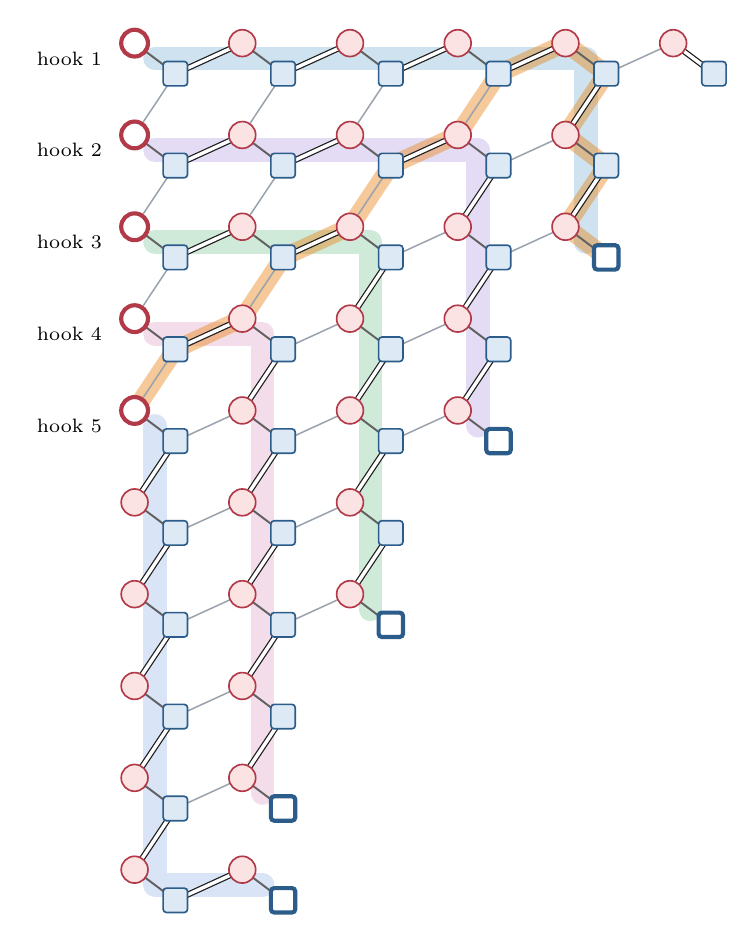
\begin{tikzpicture}[]
\begin{scope}[on background layer]
\draw[hook,rowA] (0.000,0.000) -- (1.368,0.000) -- (2.736,0.000) -- (4.104,0.000) -- (5.472,0.000) -- (5.472,-1.166) -- (5.472,-2.333);
\draw[hook,rowB] (0.000,-1.166) -- (1.368,-1.166) -- (2.736,-1.166) -- (4.104,-1.166) -- (4.104,-2.333) -- (4.104,-3.499) -- (4.104,-4.666);
\draw[hook,rowC] (0.000,-2.333) -- (1.368,-2.333) -- (2.736,-2.333) -- (2.736,-3.499) -- (2.736,-4.666) -- (2.736,-5.832) -- (2.736,-6.998);
\draw[hook,rowD] (0.000,-3.499) -- (1.368,-3.499) -- (1.368,-4.666) -- (1.368,-5.832) -- (1.368,-6.998) -- (1.368,-8.165) -- (1.368,-9.331);
\draw[hook,rowE] (0.000,-4.666) -- (0.000,-5.832) -- (0.000,-6.998) -- (0.000,-8.165) -- (0.000,-9.331) -- (0.000,-10.498) -- (1.368,-10.498);
\draw[sap] (-0.259,-4.471) -- (0.259,-3.694) -- (1.109,-3.305) -- (1.627,-2.527) -- (2.477,-2.138) -- (2.995,-1.361) -- (3.845,-0.972) -- (4.363,-0.194) -- (5.213,0.194) -- (5.731,-0.194) -- (5.213,-0.972) -- (5.731,-1.361) -- (5.213,-2.138) -- (5.731,-2.527);
\end{scope}
\draw[couple] (-0.259,-10.303) -- (0.259,-9.526);
\draw[pedge] (-0.259,-10.303) -- (0.259,-10.692);
\draw[couple] (-0.259,-9.137) -- (0.259,-8.359);
\draw[pedge] (-0.259,-9.137) -- (0.259,-9.526);
\draw[couple] (-0.259,-7.970) -- (0.259,-7.193);
\draw[pedge] (-0.259,-7.970) -- (0.259,-8.359);
\draw[couple] (-0.259,-6.804) -- (0.259,-6.026);
\draw[pedge] (-0.259,-6.804) -- (0.259,-7.193);
\draw[couple] (-0.259,-5.638) -- (0.259,-4.860);
\draw[pedge] (-0.259,-5.638) -- (0.259,-6.026);
\draw[edge] (-0.259,-4.471) -- (0.259,-3.694);
\draw[pedge] (-0.259,-4.471) -- (0.259,-4.860);
\draw[edge] (-0.259,-3.305) -- (0.259,-2.527);
\draw[pedge] (-0.259,-3.305) -- (0.259,-3.694);
\draw[edge] (-0.259,-2.138) -- (0.259,-1.361);
\draw[pedge] (-0.259,-2.138) -- (0.259,-2.527);
\draw[edge] (-0.259,-0.972) -- (0.259,-0.194);
\draw[pedge] (-0.259,-0.972) -- (0.259,-1.361);
\draw[pedge] (-0.259,0.194) -- (0.259,-0.194);
\draw[couple] (1.109,0.194) -- (0.259,-0.194);
\draw[pedge] (1.109,0.194) -- (1.627,-0.194);
\draw[couple] (2.477,0.194) -- (1.627,-0.194);
\draw[pedge] (2.477,0.194) -- (2.995,-0.194);
\draw[couple] (3.845,0.194) -- (2.995,-0.194);
\draw[pedge] (3.845,0.194) -- (4.363,-0.194);
\draw[couple] (5.213,0.194) -- (4.363,-0.194);
\draw[pedge] (5.213,0.194) -- (5.731,-0.194);
\draw[edge] (6.581,0.194) -- (5.731,-0.194);
\draw[couple] (6.581,0.194) -- (7.099,-0.194);
\draw[couple] (1.109,-0.972) -- (0.259,-1.361);
\draw[edge] (1.109,-0.972) -- (1.627,-0.194);
\draw[pedge] (1.109,-0.972) -- (1.627,-1.361);
\draw[couple] (2.477,-0.972) -- (1.627,-1.361);
\draw[edge] (2.477,-0.972) -- (2.995,-0.194);
\draw[pedge] (2.477,-0.972) -- (2.995,-1.361);
\draw[couple] (3.845,-0.972) -- (2.995,-1.361);
\draw[edge] (3.845,-0.972) -- (4.363,-0.194);
\draw[pedge] (3.845,-0.972) -- (4.363,-1.361);
\draw[edge] (5.213,-0.972) -- (4.363,-1.361);
\draw[couple] (5.213,-0.972) -- (5.731,-0.194);
\draw[pedge] (5.213,-0.972) -- (5.731,-1.361);
\draw[couple] (1.109,-2.138) -- (0.259,-2.527);
\draw[edge] (1.109,-2.138) -- (1.627,-1.361);
\draw[pedge] (1.109,-2.138) -- (1.627,-2.527);
\draw[couple] (2.477,-2.138) -- (1.627,-2.527);
\draw[edge] (2.477,-2.138) -- (2.995,-1.361);
\draw[pedge] (2.477,-2.138) -- (2.995,-2.527);
\draw[edge] (3.845,-2.138) -- (2.995,-2.527);
\draw[couple] (3.845,-2.138) -- (4.363,-1.361);
\draw[pedge] (3.845,-2.138) -- (4.363,-2.527);
\draw[edge] (5.213,-2.138) -- (4.363,-2.527);
\draw[couple] (5.213,-2.138) -- (5.731,-1.361);
\draw[pedge] (5.213,-2.138) -- (5.731,-2.527);
\draw[couple] (1.109,-3.305) -- (0.259,-3.694);
\draw[edge] (1.109,-3.305) -- (1.627,-2.527);
\draw[pedge] (1.109,-3.305) -- (1.627,-3.694);
\draw[edge] (2.477,-3.305) -- (1.627,-3.694);
\draw[couple] (2.477,-3.305) -- (2.995,-2.527);
\draw[pedge] (2.477,-3.305) -- (2.995,-3.694);
\draw[edge] (3.845,-3.305) -- (2.995,-3.694);
\draw[couple] (3.845,-3.305) -- (4.363,-2.527);
\draw[pedge] (3.845,-3.305) -- (4.363,-3.694);
\draw[edge] (1.109,-4.471) -- (0.259,-4.860);
\draw[couple] (1.109,-4.471) -- (1.627,-3.694);
\draw[pedge] (1.109,-4.471) -- (1.627,-4.860);
\draw[edge] (2.477,-4.471) -- (1.627,-4.860);
\draw[couple] (2.477,-4.471) -- (2.995,-3.694);
\draw[pedge] (2.477,-4.471) -- (2.995,-4.860);
\draw[edge] (3.845,-4.471) -- (2.995,-4.860);
\draw[couple] (3.845,-4.471) -- (4.363,-3.694);
\draw[pedge] (3.845,-4.471) -- (4.363,-4.860);
\draw[edge] (1.109,-5.638) -- (0.259,-6.026);
\draw[couple] (1.109,-5.638) -- (1.627,-4.860);
\draw[pedge] (1.109,-5.638) -- (1.627,-6.026);
\draw[edge] (2.477,-5.638) -- (1.627,-6.026);
\draw[couple] (2.477,-5.638) -- (2.995,-4.860);
\draw[pedge] (2.477,-5.638) -- (2.995,-6.026);
\draw[edge] (1.109,-6.804) -- (0.259,-7.193);
\draw[couple] (1.109,-6.804) -- (1.627,-6.026);
\draw[pedge] (1.109,-6.804) -- (1.627,-7.193);
\draw[edge] (2.477,-6.804) -- (1.627,-7.193);
\draw[couple] (2.477,-6.804) -- (2.995,-6.026);
\draw[pedge] (2.477,-6.804) -- (2.995,-7.193);
\draw[edge] (1.109,-7.970) -- (0.259,-8.359);
\draw[couple] (1.109,-7.970) -- (1.627,-7.193);
\draw[pedge] (1.109,-7.970) -- (1.627,-8.359);
\draw[edge] (1.109,-9.137) -- (0.259,-9.526);
\draw[couple] (1.109,-9.137) -- (1.627,-8.359);
\draw[pedge] (1.109,-9.137) -- (1.627,-9.526);
\draw[couple] (1.109,-10.303) -- (0.259,-10.692);
\draw[pedge] (1.109,-10.303) -- (1.627,-10.692);
\node[small girl] at (-0.259,-10.303) {};
\node[small girl] at (-0.259,-9.137) {};
\node[small girl] at (-0.259,-7.970) {};
\node[small girl] at (-0.259,-6.804) {};
\node[small girl] at (-0.259,-5.638) {};
\node[small girl,free] at (-0.259,-4.471) {};
\node[small girl,free] at (-0.259,-3.305) {};
\node[small girl,free] at (-0.259,-2.138) {};
\node[small girl,free] at (-0.259,-0.972) {};
\node[small girl,free] at (-0.259,0.194) {};
\node[small girl] at (1.109,0.194) {};
\node[small girl] at (2.477,0.194) {};
\node[small girl] at (3.845,0.194) {};
\node[small girl] at (5.213,0.194) {};
\node[small girl] at (6.581,0.194) {};
\node[small girl] at (1.109,-0.972) {};
\node[small girl] at (2.477,-0.972) {};
\node[small girl] at (3.845,-0.972) {};
\node[small girl] at (5.213,-0.972) {};
\node[small girl] at (1.109,-2.138) {};
\node[small girl] at (2.477,-2.138) {};
\node[small girl] at (3.845,-2.138) {};
\node[small girl] at (5.213,-2.138) {};
\node[small girl] at (1.109,-3.305) {};
\node[small girl] at (2.477,-3.305) {};
\node[small girl] at (3.845,-3.305) {};
\node[small girl] at (1.109,-4.471) {};
\node[small girl] at (2.477,-4.471) {};
\node[small girl] at (3.845,-4.471) {};
\node[small girl] at (1.109,-5.638) {};
\node[small girl] at (2.477,-5.638) {};
\node[small girl] at (1.109,-6.804) {};
\node[small girl] at (2.477,-6.804) {};
\node[small girl] at (1.109,-7.970) {};
\node[small girl] at (1.109,-9.137) {};
\node[small girl] at (1.109,-10.303) {};
\node[small boy] at (0.259,-0.194) {};
\node[small boy] at (1.627,-0.194) {};
\node[small boy] at (2.995,-0.194) {};
\node[small boy] at (4.363,-0.194) {};
\node[small boy] at (5.731,-0.194) {};
\node[small boy] at (7.099,-0.194) {};
\node[small boy] at (0.259,-1.361) {};
\node[small boy] at (1.627,-1.361) {};
\node[small boy] at (2.995,-1.361) {};
\node[small boy] at (4.363,-1.361) {};
\node[small boy] at (5.731,-1.361) {};
\node[small boy] at (0.259,-2.527) {};
\node[small boy] at (1.627,-2.527) {};
\node[small boy] at (2.995,-2.527) {};
\node[small boy] at (4.363,-2.527) {};
\node[small boy,free] at (5.731,-2.527) {};
\node[small boy] at (0.259,-3.694) {};
\node[small boy] at (1.627,-3.694) {};
\node[small boy] at (2.995,-3.694) {};
\node[small boy] at (4.363,-3.694) {};
\node[small boy] at (0.259,-4.860) {};
\node[small boy] at (1.627,-4.860) {};
\node[small boy] at (2.995,-4.860) {};
\node[small boy,free] at (4.363,-4.860) {};
\node[small boy] at (0.259,-6.026) {};
\node[small boy] at (1.627,-6.026) {};
\node[small boy] at (2.995,-6.026) {};
\node[small boy] at (0.259,-7.193) {};
\node[small boy] at (1.627,-7.193) {};
\node[small boy,free] at (2.995,-7.193) {};
\node[small boy] at (0.259,-8.359) {};
\node[small boy] at (1.627,-8.359) {};
\node[small boy] at (0.259,-9.526) {};
\node[small boy,free] at (1.627,-9.526) {};
\node[small boy] at (0.259,-10.692) {};
\node[small boy,free] at (1.627,-10.692) {};
\node[font=\scriptsize,anchor=east] at (-0.550,0.000) {hook 1};
\node[font=\scriptsize,anchor=east] at (-0.550,-1.166) {hook 2};
\node[font=\scriptsize,anchor=east] at (-0.550,-2.333) {hook 3};
\node[font=\scriptsize,anchor=east] at (-0.550,-3.499) {hook 4};
\node[font=\scriptsize,anchor=east] at (-0.550,-4.666) {hook 5};
\end{tikzpicture}

\caption{State~$f=5$ of $\Gam_{11}$, before the round at level~$L=7$. The
five hooks (coloured) run east along their rows and turn south at
columns~$5,4,3,2,1$. Cells in columns~$6$ and beyond are retired. All
five hooks have $7$ cells. For instance cell~$(7,2)$ lies in
hook~$\min(7,6-2)=4$, at position~$2+\max(0,7+2-6)=5$, as
Lemma~\ref{lem:hooks}(a) says. The orange staircase is the SAP that
Algorithm~H finds: it starts at the free girl of hook~5 and climbs to the
free boy of hook~1.}
\label{fig:hooks}
\end{figure}

\begin{lemma}
\label{lem:hooks}
Let $1\le f\le n-1$ and $L=n+1-f$.
\begin{enumerate}[label=(\alph*)]
\item The hooks are disjoint, and their cells are exactly the cells in
  columns~$1,\ldots,f$ together with the corner cell. An alive cell
  $(a,c)$ other than the corner lies in hook~$x=\min(a,f+1-c)$, at position
  $y=c+\max(0,a+c-f-1)$ along it; the corner is at position~$L$ of
  hook~$f$.
\item Consecutive cells of a hook are joined by a horizontal or vertical
  edge of $\Gam_n$, so $M_f$ is a matching of $\Gam_n$.
\item Hook~$x$ has $\max(\ell_x,L)$ cells. Hence hooks~$1,\ldots,k-1$
  have more than $L$ cells and hooks~$k,\ldots,f$ have exactly $L$ cells,
  where
  \[
      k=\max(1,f-L),\qquad m=f-k+1=\min(f,L+1).
  \]
\item $M_{n-1}$ is the matching produced by~\Hs1.
\end{enumerate}
\end{lemma}

\begin{proof}
(a) A cell~$(a,c)$ with $c\le f$ and $a+c\le f+1$ lies in row~$a$ at or
before the corner column~$f+1-a$ of hook~$a$, so it belongs to hook~$a$ at
position~$c$. If $a+c>f+1$, the hook whose corner column is $c$ is hook
$x=f+1-c<a$; since columns are top-justified, cell~$(x,c)$ exists, so
hook~$x$ turns south at $(x,c)$ and contains $(a,c)$ at position
$c+(a-x)$, unless $(a,c)$ is the corner. Conversely every hook stays in
columns~$\le f$ apart from the corner, and the two cases above assign each
cell to only one hook.

(b) East steps use horizontal edges and south steps use vertical edges;
the omitted edge would lead into the corner, which is entered from its
left neighbour $(n-1,1)$ instead.

(c) Write $c=f+1-x$, and note that $2\ell_x\ge n+1-x$ always. If
$\ell_x<c$, hook~$x$ is row~$x$; then $x\le f-\ell_x$, so
$2\ell_x\ge n+1-f+\ell_x$, that is, $\ell_x\ge L$. Otherwise, if $x<f$, hook
$x$ consists of $c$ cells of row~$x$ followed by the cells of column~$c$
below it. Column~$c\ge2$ ends at row~$n+2-2c$ (the corner is not counted),
so the hook has $c+(n+2-2c-x)=n+2-c-x=L$ cells. The last hook has
$1+(n-1-f)+1=L$ cells. In this second case~$\ell_x\le L$ as well: for
$x=n-1$ we have $\ell_x=2=L$, and otherwise $2\ell_x\le n+2-x$, whereas
$\ell_x\ge L+1$ and $\ell_x\ge c$ would give $2\ell_x\ge n+3-x$. Finally,
$\ell_x\ge L+1=n+2-f$ if and only if $n+2-x\ge2(n+2-f)$, that is,
$x\le f-L-1$.

(d) For $f=n-1$ the corner column of hook~$x$ is $n-x$, which exceeds
$\ell_x$ when $x\le n-3$; for the last two rows the definition also gives
the whole row. So $M_{n-1}$ couples the horizontal edges, as in
Proposition~\ref{prop:gamma}.
\end{proof}

Write $y(a,c)$ for the position of an alive cell, as given by part~(a).
Two facts about it drive the next two lemmas: $y$ never decreases when we
move from an alive cell to the alive cell below it or to its right, and it
increases by exactly one from each cell of a hook to the next. (For the
corner, $y=L$; its left neighbour has position~$L-1$, and the cell above it,
$(n-2,2)$, also has position~$L$.)

\subsection{No shortcuts}

The graph has many edges that the hooks do not use, and some of them will
be needed in later rounds. The next lemma shows that none of them
creates a shorter augmenting path now.

\begin{lemma}
\label{lem:levels}
In the matching $M_f$, the girl of an alive cell at position~$y$ of its
hook is at distance $2(y-1)$ from the free girls, and its boy at distance
$2y-1$. No retired vertex can be reached by an alternating path from a
free girl. Consequently the dag has level~$L$, and its SAPs end at the
free boys of hooks~$k,\ldots,f$.
\end{lemma}

\begin{proof}
First, retired vertices. A retired boy~$b_{a,c}$ can be entered only from
the girl to his right or the girl below him, since his own girl is his
mate. Both lie in retired cells, being in column~$c$ or $c+1$, beyond
column~$f$. (When $f=1$ the corner is alive and lies below the retired
cell~$(n-2,2)$; this is one place where the omitted edge matters.) A
retired girl can be entered only from her own boy. So no alternating path
from a free girl ever reaches a retired vertex.

Now follow an alternating path from a free girl. A step from a girl to a
boy uses an edge outside $M_f$, which goes from cell~$(a,c)$ to the same
cell, to $(a,c-1)$, or to $(a-1,c)$; by the monotonicity of positions it
does not increase the position. A step from a boy to a girl uses a couple
of $M_f$, and so increases the position by exactly one. The path starts
at position~1, so a boy at position~$y$ is reached only after at least
$y-1$ couples, that is, after at least $2y-1$ edges. The beginning of his
own hook reaches him in exactly that many. The argument for girls is the
same.

Free boys are the last boys of the hooks, at positions $\max(\ell_x,L)\ge
L$. The smallest distance to one of them is therefore $2L-1$, attained
exactly by hooks~$k,\ldots,f$.
\end{proof}

\subsection{The forced search}

Now the input order enters. Fig.~\ref{fig:straight} shows a dag of a
staircase graph with each hook drawn as a straight row; the positions
become the columns, which are exactly the levels of the dag.

\begin{figure}[ht]
\centering
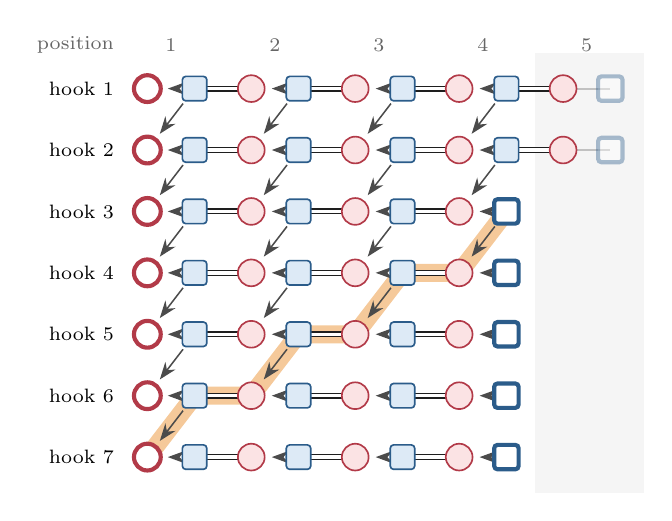
\begin{tikzpicture}[]
\begin{scope}[on background layer]
\draw[sap] (-0.300,-4.680) -- (0.300,-3.900) -- (1.020,-3.900) -- (1.620,-3.120) -- (2.340,-3.120) -- (2.940,-2.340) -- (3.660,-2.340) -- (4.260,-1.560);
\fill[black!4] (4.620,0.450) rectangle (6.006,-5.130);
\end{scope}
\draw[couple] (1.620,-4.680) -- (2.340,-4.680);
\draw[couple] (0.300,-4.680) -- (1.020,-4.680);
\draw[couple] (0.300,0.000) -- (1.020,0.000);
\draw[couple] (1.620,0.000) -- (2.340,0.000);
\draw[couple] (2.940,0.000) -- (3.660,0.000);
\draw[couple] (4.260,0.000) -- (4.980,0.000);
\draw[couple] (0.300,-0.780) -- (1.020,-0.780);
\draw[couple] (1.620,-0.780) -- (2.340,-0.780);
\draw[couple] (2.940,-0.780) -- (3.660,-0.780);
\draw[couple] (4.260,-0.780) -- (4.980,-0.780);
\draw[couple] (0.300,-1.560) -- (1.020,-1.560);
\draw[couple] (1.620,-1.560) -- (2.340,-1.560);
\draw[couple] (2.940,-1.560) -- (3.660,-1.560);
\draw[couple] (0.300,-2.340) -- (1.020,-2.340);
\draw[couple] (1.620,-2.340) -- (2.340,-2.340);
\draw[couple] (2.940,-2.340) -- (3.660,-2.340);
\draw[couple] (0.300,-3.120) -- (1.020,-3.120);
\draw[couple] (1.620,-3.120) -- (2.340,-3.120);
\draw[couple] (0.300,-3.900) -- (1.020,-3.900);
\draw[couple] (2.940,-3.120) -- (3.660,-3.120);
\draw[couple] (1.620,-3.900) -- (2.340,-3.900);
\draw[couple] (2.940,-3.900) -- (3.660,-3.900);
\draw[couple] (2.940,-4.680) -- (3.660,-4.680);
\draw[arc,shorten >=2.6mm,shorten <=2.4mm] (0.300,0.000) -- (-0.300,-0.780);
\draw[arc,shorten >=2.6mm,shorten <=2.4mm] (0.300,0.000) -- (-0.300,0.000);
\draw[arc,shorten >=2.6mm,shorten <=2.4mm] (0.300,-0.780) -- (-0.300,-1.560);
\draw[arc,shorten >=2.6mm,shorten <=2.4mm] (0.300,-0.780) -- (-0.300,-0.780);
\draw[arc,shorten >=2.6mm,shorten <=2.4mm] (0.300,-1.560) -- (-0.300,-2.340);
\draw[arc,shorten >=2.6mm,shorten <=2.4mm] (0.300,-1.560) -- (-0.300,-1.560);
\draw[arc,shorten >=2.6mm,shorten <=2.4mm] (0.300,-2.340) -- (-0.300,-3.120);
\draw[arc,shorten >=2.6mm,shorten <=2.4mm] (0.300,-2.340) -- (-0.300,-2.340);
\draw[arc,shorten >=2.6mm,shorten <=2.4mm] (0.300,-3.120) -- (-0.300,-3.900);
\draw[arc,shorten >=2.6mm,shorten <=2.4mm] (0.300,-3.120) -- (-0.300,-3.120);
\draw[arc,shorten >=2.6mm,shorten <=2.4mm] (0.300,-3.900) -- (-0.300,-4.680);
\draw[arc,shorten >=2.6mm,shorten <=2.4mm] (0.300,-3.900) -- (-0.300,-3.900);
\draw[arc,shorten >=2.6mm,shorten <=2.4mm] (0.300,-4.680) -- (-0.300,-4.680);
\draw[arc,shorten >=2.6mm,shorten <=2.4mm] (1.620,0.000) -- (1.020,-0.780);
\draw[arc,shorten >=2.6mm,shorten <=2.4mm] (1.620,0.000) -- (1.020,0.000);
\draw[arc,shorten >=2.6mm,shorten <=2.4mm] (1.620,-0.780) -- (1.020,-1.560);
\draw[arc,shorten >=2.6mm,shorten <=2.4mm] (1.620,-0.780) -- (1.020,-0.780);
\draw[arc,shorten >=2.6mm,shorten <=2.4mm] (1.620,-1.560) -- (1.020,-2.340);
\draw[arc,shorten >=2.6mm,shorten <=2.4mm] (1.620,-1.560) -- (1.020,-1.560);
\draw[arc,shorten >=2.6mm,shorten <=2.4mm] (1.620,-2.340) -- (1.020,-3.120);
\draw[arc,shorten >=2.6mm,shorten <=2.4mm] (1.620,-2.340) -- (1.020,-2.340);
\draw[arc,shorten >=2.6mm,shorten <=2.4mm] (1.620,-3.120) -- (1.020,-3.900);
\draw[arc,shorten >=2.6mm,shorten <=2.4mm] (1.620,-3.120) -- (1.020,-3.120);
\draw[arc,shorten >=2.6mm,shorten <=2.4mm] (1.620,-3.900) -- (1.020,-3.900);
\draw[arc,shorten >=2.6mm,shorten <=2.4mm] (1.620,-4.680) -- (1.020,-4.680);
\draw[arc,shorten >=2.6mm,shorten <=2.4mm] (2.940,0.000) -- (2.340,-0.780);
\draw[arc,shorten >=2.6mm,shorten <=2.4mm] (2.940,0.000) -- (2.340,0.000);
\draw[arc,shorten >=2.6mm,shorten <=2.4mm] (2.940,-0.780) -- (2.340,-1.560);
\draw[arc,shorten >=2.6mm,shorten <=2.4mm] (2.940,-0.780) -- (2.340,-0.780);
\draw[arc,shorten >=2.6mm,shorten <=2.4mm] (2.940,-1.560) -- (2.340,-2.340);
\draw[arc,shorten >=2.6mm,shorten <=2.4mm] (2.940,-1.560) -- (2.340,-1.560);
\draw[arc,shorten >=2.6mm,shorten <=2.4mm] (2.940,-2.340) -- (2.340,-3.120);
\draw[arc,shorten >=2.6mm,shorten <=2.4mm] (2.940,-2.340) -- (2.340,-2.340);
\draw[arc,shorten >=2.6mm,shorten <=2.4mm] (2.940,-3.120) -- (2.340,-3.120);
\draw[arc,shorten >=2.6mm,shorten <=2.4mm] (2.940,-3.900) -- (2.340,-3.900);
\draw[arc,shorten >=2.6mm,shorten <=2.4mm] (2.940,-4.680) -- (2.340,-4.680);
\draw[arc,shorten >=2.6mm,shorten <=2.4mm] (4.260,0.000) -- (3.660,-0.780);
\draw[arc,shorten >=2.6mm,shorten <=2.4mm] (4.260,0.000) -- (3.660,0.000);
\draw[arc,shorten >=2.6mm,shorten <=2.4mm] (4.260,-0.780) -- (3.660,-1.560);
\draw[arc,shorten >=2.6mm,shorten <=2.4mm] (4.260,-0.780) -- (3.660,-0.780);
\draw[arc,shorten >=2.6mm,shorten <=2.4mm] (4.260,-1.560) -- (3.660,-2.340);
\draw[arc,shorten >=2.6mm,shorten <=2.4mm] (4.260,-1.560) -- (3.660,-1.560);
\draw[arc,shorten >=2.6mm,shorten <=2.4mm] (4.260,-2.340) -- (3.660,-2.340);
\draw[arc,shorten >=2.6mm,shorten <=2.4mm] (4.260,-3.120) -- (3.660,-3.120);
\draw[arc,shorten >=2.6mm,shorten <=2.4mm] (4.260,-3.900) -- (3.660,-3.900);
\draw[arc,shorten >=2.6mm,shorten <=2.4mm] (4.260,-4.680) -- (3.660,-4.680);
\draw[pedge,opacity=.35] (4.980,0.000) -- (5.580,0.000);
\draw[pedge,opacity=.35] (4.980,-0.780) -- (5.580,-0.780);
\node[small girl,free] at (-0.300,0.000) {};
\node[small girl] at (1.020,0.000) {};
\node[small girl] at (2.340,0.000) {};
\node[small girl] at (3.660,0.000) {};
\node[small girl] at (4.980,0.000) {};
\node[small girl,free] at (-0.300,-0.780) {};
\node[small girl] at (1.020,-0.780) {};
\node[small girl] at (2.340,-0.780) {};
\node[small girl] at (3.660,-0.780) {};
\node[small girl] at (4.980,-0.780) {};
\node[small girl,free] at (-0.300,-1.560) {};
\node[small girl] at (1.020,-1.560) {};
\node[small girl] at (2.340,-1.560) {};
\node[small girl] at (3.660,-1.560) {};
\node[small girl,free] at (-0.300,-2.340) {};
\node[small girl] at (1.020,-2.340) {};
\node[small girl] at (2.340,-2.340) {};
\node[small girl] at (3.660,-2.340) {};
\node[small girl,free] at (-0.300,-3.120) {};
\node[small girl] at (1.020,-3.120) {};
\node[small girl] at (2.340,-3.120) {};
\node[small girl] at (3.660,-3.120) {};
\node[small girl,free] at (-0.300,-3.900) {};
\node[small girl] at (1.020,-3.900) {};
\node[small girl] at (2.340,-3.900) {};
\node[small girl] at (3.660,-3.900) {};
\node[small girl,free] at (-0.300,-4.680) {};
\node[small girl] at (1.020,-4.680) {};
\node[small girl] at (2.340,-4.680) {};
\node[small girl] at (3.660,-4.680) {};
\node[small boy] at (0.300,0.000) {};
\node[small boy] at (1.620,0.000) {};
\node[small boy] at (2.940,0.000) {};
\node[small boy] at (4.260,0.000) {};
\node[small boy,free,opacity=.4] at (5.580,0.000) {};
\node[small boy] at (0.300,-0.780) {};
\node[small boy] at (1.620,-0.780) {};
\node[small boy] at (2.940,-0.780) {};
\node[small boy] at (4.260,-0.780) {};
\node[small boy,free,opacity=.4] at (5.580,-0.780) {};
\node[small boy] at (0.300,-1.560) {};
\node[small boy] at (1.620,-1.560) {};
\node[small boy] at (2.940,-1.560) {};
\node[small boy,free] at (4.260,-1.560) {};
\node[small boy] at (0.300,-2.340) {};
\node[small boy] at (1.620,-2.340) {};
\node[small boy] at (2.940,-2.340) {};
\node[small boy,free] at (4.260,-2.340) {};
\node[small boy] at (0.300,-3.120) {};
\node[small boy] at (1.620,-3.120) {};
\node[small boy] at (2.940,-3.120) {};
\node[small boy,free] at (4.260,-3.120) {};
\node[small boy] at (0.300,-3.900) {};
\node[small boy] at (1.620,-3.900) {};
\node[small boy] at (2.940,-3.900) {};
\node[small boy,free] at (4.260,-3.900) {};
\node[small boy] at (0.300,-4.680) {};
\node[small boy] at (1.620,-4.680) {};
\node[small boy] at (2.940,-4.680) {};
\node[small boy,free] at (4.260,-4.680) {};
\node[font=\scriptsize,anchor=east] at (-0.600,0.000) {hook 1};
\node[font=\scriptsize,anchor=east] at (-0.600,-0.780) {hook 2};
\node[font=\scriptsize,anchor=east] at (-0.600,-1.560) {hook 3};
\node[font=\scriptsize,anchor=east] at (-0.600,-2.340) {hook 4};
\node[font=\scriptsize,anchor=east] at (-0.600,-3.120) {hook 5};
\node[font=\scriptsize,anchor=east] at (-0.600,-3.900) {hook 6};
\node[font=\scriptsize,anchor=east] at (-0.600,-4.680) {hook 7};
\node[font=\scriptsize,text=black!60] at (0.000,0.550) {1};
\node[font=\scriptsize,text=black!60] at (1.320,0.550) {2};
\node[font=\scriptsize,text=black!60] at (2.640,0.550) {3};
\node[font=\scriptsize,text=black!60] at (3.960,0.550) {4};
\node[font=\scriptsize,text=black!60] at (5.280,0.550) {5};
\node[font=\scriptsize,text=black!60,anchor=east] at (-0.600,0.550) {position};
\end{tikzpicture}

\caption{The dag of the round at level~$L=4$ of $\Gam_{10}$ (state~$f=7$),
with the hooks straightened. Arrows are the arcs of $\A{BLINK}$, from a
boy to a girl one level down: every boy has an arc to his own girl, and
the boy at position~$y$ of hook~$x$ also has an arc to the girl below him
when $x+y\le7$; that arc comes first in $\A{BLINK}$. Hooks~1 and~2 have
more than $L$ cells (the shaded column lies beyond the dag). The search
starts at the free boy of hook~3, the first hook with exactly $L$ cells,
and always takes the first arc, so it goes down a staircase to the last
free girl.}
\label{fig:straight}
\end{figure}

\begin{lemma}
\label{lem:bfs}
Suppose a round starts with the matching $M_f$ and with the free girls in
\A{QUEUE} in hook order. Then each level~$G_j$ of the dag is listed in hook
order, and for the boy~$b$ at position~$y\le L$ of hook~$x$,
\[
  \A{BLINK}[b]=\begin{cases}
   (\text{girl at position~$y$ of hook~$x+1$},\ \text{girl at position~$y$ of hook~$x$}),&\text{if } x+y\le f;\\
   (\text{girl at position~$y$ of hook~$x$}),&\text{if } x+y>f.
  \end{cases}
\]
The roots of the depth-first search are the free boys of hooks
$k,k+1,\ldots,f$, in this order.
\end{lemma}

\begin{proof}
Let $b=b_{a,c}$ lie at position~$y$ of hook~$x$. By
Lemma~\ref{lem:levels}, the girls one level below $b$ are those at
position~$y$. Of his three possible neighbours, his own girl qualifies;
the girl to his right does not, since her position is larger; and the girl
below him, $g_{a+1,c}$, if she is adjacent to him, qualifies exactly when
the two cells have the same position. By the formula of
Lemma~\ref{lem:hooks}(a) that means $a+c\le f$, with one exception: the
corner has the same position as the cell above it, but the edge between
them is the omitted one, which is the main reason for omitting it. When
$a+c\le f$, then $(a,c)$ lies in the first part of hook~$a$, so $c=y\le L$,
and $(a+1)+2c\le f+1+L=n+2$; hence cell~$(a+1,c)$ exists, and it is not the
corner because $a+c\le f<n$. Also $(a,c)$ is at
position~$c$ of hook~$a$, so $a+c\le f$ is the condition $x+y\le f$, and
$g_{a+1,c}$ is at position~$y$ of hook~$x+1$.

Now argue by induction on $j$ that $G_j$ is in hook order. For $j=0$ this
is the hypothesis. When the girls of $G_j$ are scanned, the girl of hook
$x$ meets at most three boys: her own boy; her left boy, whose position is
smaller, so that he is already in the dag at a lower level and step~\Hs6
ignores him; and her upper boy, whose position is at most hers. (On the
vertical part of a hook her upper boy is her mate, at the level below.) The
only girls of $G_j$ adjacent to her own boy are herself and the girl of
hook~$x+1$, who comes later; so she is the one who discovers him. Thus $B_{j+1}$
is discovered in hook order, and so is $G_{j+1}$, which consists of their
mates. When the girl of hook~$x+1$ later meets the same boy as her upper
boy, step~\Hs6 inserts her at the head of his list, which gives the stated
order of $\A{BLINK}$.

At level~$L$ the boys of hooks~$1,\ldots,k-1$ are matched and are
discovered before the first free boy (in hook~$k$), so they enter the
dag; the free boys of hooks~$k,\ldots,f$ follow in order and become the
roots.
\end{proof}

\begin{lemma}
\label{lem:dfs}
Under the hypotheses of Lemma~\ref{lem:bfs}, the round finds exactly one
SAP. Its free girl is the last girl in \A{QUEUE}, and afterwards the matching
is $M_{f-1}$, with the remaining free girls still in hook order.
\end{lemma}

\begin{proof}
Write $\langle x,y\rangle$ for position~$y$ of hook~$x$, and recall that hooks
$k,\ldots,f$ have exactly $L$ cells and $f-k\le L$.

\emph{The first root.} The search starts at the boy~$\langle k,L\rangle$ and always
follows the first remaining arc. Suppose first that $f\ge L+1$, so that
$k=f-L$ and $k+L=f$. Then the first arc leads to the girl~$\langle k+1,L\rangle$; her
mate is the boy~$\langle k+1,L-1\rangle$, whose hook and position again add up to $f$,
so the next arc leads to the girl~$\langle k+2,L-1\rangle$, and so on down the
staircase
\[
   \text{boy }\langle i,f-i\rangle\ \to\ \text{girl }\langle i+1,f-i\rangle\ \db\ \text{boy }\langle i+1,f-i-1\rangle
   \qquad(i=k,k+1,\ldots,f-1),
\]
ending at the girl~$\langle f,1\rangle$, who is free. If instead $f\le L$, then $k=1$,
and the search first walks backwards along hook~1 (each boy~$\langle 1,y\rangle$ with
$1+y>f$ has only his own girl) until it reaches the boy~$\langle 1,f-1\rangle$; from
there it descends the same staircase. In both cases the SAP ends at the
free girl of hook~$f$, the last girl in \A{QUEUE}, so step~\Hs{16} leaves the
order of the others unchanged.

\emph{The other roots fail.} The SAP passes through the girl~$\langle i,f+1-i\rangle$
of every hook~$i$ with $k<i\le f$. The root $\langle i,L\rangle$ of such a hook has only
one arc at each position~$y$ with $i+y>f$, namely to its own girl. Following
these single arcs, it reaches the boy~$\langle i,f+1-i\rangle$, whose only girl has been
deleted. Every list on the way is now empty, and step~\Hs{15} backs up all
the way: the root fails. So the round has exactly one SAP.

\emph{The new matching.} Augmenting dissolves, in each hook~$i$ with
$k<i<f$, the couple between positions $f-i$ and $f+1-i$, and couples
instead the boy at position~$f-i$ of hook~$i$ to the girl at position
$f-i$ of hook~$i+1$, for $k\le i<f$. Reading along the new couples, the
new hook~$i$ therefore consists of the first $f-i$ cells of the old hook
$i$, followed by the cells of the old hook~$i+1$ from position~$f-i$ on;
the remaining cells of the old hook~$i$ have passed to hook~$i-1$, and
the old hook~$f$ has been absorbed into hook~$f-1$. When $f\le L$, the
cells of hook~1 at positions $f,\ldots,L$, which the search walked
through, become coupled to themselves, that is, retired. Now compare
with the definition. In state~$f$, hook~$i+1$ has corner column~$f-i$, so
the new hook~$i$ runs east along row~$i$ to column~$f-i$ and then south:
it is hook~$i$ of state~$f-1$. The cells that retire are the alive cells
of column~$f$ other than the corner (which stays alive when $f=2$). Hooks~$1,\ldots,k-1$ are untouched whole rows, and they
are whole rows in state~$f-1$ too: for them $\ell_x\ge L+1=n+2-f$, so their
new corner column satisfies $f-x\ge n+2-x-\ell_x\ge\ell_x$, and if equality
holds then $x+2\ell_x=n+2$ and there is no cell below $(x,\ell_x)$. So the
new matching is $M_{f-1}$. For $f=1$ the search walks back along the single
hook and produces the perfect matching~$M_0$.
\end{proof}

Searched on its own, the root of each of the hooks~$k+1,\ldots,f$ would
find a SAP along its own hook. But \A{MARKED} lists the roots in hook
order, so the root of hook~$k$ goes first, and because the first arc of
each \A{BLINK} list points one hook down, its path takes the girl at
position~$f+1-i$ from every later hook~$i$. Each later root must pass
through that girl, so it fails.

\begin{lthm}{S}
On the ordered graph $\Gam_n$, Algorithm~H performs exactly $n$ rounds.
For $L=2,3,\ldots,n$, the round at level~$L$ starts with $f=n+1-L$ free
girls and finds exactly one SAP. The final matching consists of the
inside edges.
\end{lthm}

\begin{proof}
By Proposition~\ref{prop:gamma} and Lemma~\ref{lem:hooks}(d), step~\Hs1
produces $M_{n-1}$ with the free girls in hook order. Apply
Lemmas~\ref{lem:levels}--\ref{lem:dfs} for $f=n-1,n-2,\ldots,1$.
\end{proof}

\paragraph{Every size.}
Theorem~S gives $n$ rounds when $s=Q_n$. For $Q_n<s<Q_{n+1}$, append
$p=s-Q_n$ new girl--boy pairs to $\Gam_n$, numbered after all the old
ones. Give each new girl the list ``her own new boy, then the previous
boy,'' where the previous boy is the corner boy~$b_{n-1,2}$ for the first
new girl and the preceding new boy afterwards. Step~\Hs1 scans the new girls
first and couples each to her own boy. No old girl's list mentions a new
boy, so an alternating path from an old free girl never enters the new
pairs: to do so it would have to arrive at a boy whose mate is a new
girl. Hence every round runs exactly as on $\Gam_n$. The corner boy had
degree one, so the new graph is still planar, connected, and of maximum
degree three. For $s=1$ use a single edge, and for $s=0$ the empty
graph. Together with Section~\ref{sec:upper}, this proves Theorem~R.
\qed

\subsection{How much one path blocks}

In state~$f$ the hooks~$k,\ldots,f$ are $m=\min(f,L+1)$ disjoint SAPs, so
the largest set of disjoint SAPs has $\nu=m$ members, while Algorithm~H
takes one. The total number of SAPs in the dag grows exponentially in~$m$.

\begin{proposition}
In state~$f$, the dag of $\Gam_n$ contains exactly $2^m-1$ SAPs.
\end{proposition}

\begin{proof}
Let $N(x,y)$ be the number of dag paths from the boy at position~$y$ of
hook~$x$ down to $\bot$. By Lemma~\ref{lem:bfs},
$N(x,y)=N(x,y-1)+\Iv{x+y\le f}\,N(x+1,y-1)$, where $N(x,0)=1$ stands
for the free girl. Induction on $y$ gives $N(x,y)=2^{\min(y,f-x)}$. A root
$\langle i,L\rangle$ with $k\le i\le f$ therefore starts $2^{f-i}$ SAPs, since $f-i\le
f-k\le L$, and $\sum_{i=k}^{f}2^{f-i}=2^m-1$.
\end{proof}

Every SAP from the root of hook~$i>k$ passes through the girl at position
$f+1-i$ of that hook, which the first SAP uses. So the one SAP found by
Algorithm~H meets all $2^m-1$ SAPs, including all $m$ disjoint ones.
Lemma~\ref{lem:15ab}(b) with $\nu=m\le L+1$ in place of $f$ predicts at
least one SAP, and one is what Algorithm~H finds.

\subsection{Counting the work}
\label{sec:work}

\begin{lthm}{W}
In the round of $\Gam_n$ with $f$ free girls and level~$L=n+1-f$, with
$m=\min(f,L+1)$ as above,
\[
   W_5=3fL-n-\min(f,L),\qquad W_{13}=mL-\binom{m-1}{2},\qquad W_{11}=fL.
\]
Summed over all rounds after~\Hs1,
\[
  \sum W_5=\frac{(n-1)n(n+2)}2-Q_n+1,\qquad \sum W_{11}=\frac{(n-1)n(n+4)}6,
\]
\[
  \sum W_{13}=\begin{cases}(4u^3+21u^2+23u-6)/6,& n=2u+1,\\
                 (4u^3+15u^2+5u-12)/6,& n=2u.\end{cases}
\]
The final, unsuccessful search examines no edges.
\end{lthm}

\begin{proof}
The breadth-first search scans the girls at positions $1,\ldots,L$ of all
$f$ hooks, $fL$ girls in all, and every list entry of each. A girl has
three neighbours except that girls in column~1 have no left boy, girls in
row~1 have no upper boy, and the corner girl lacks the omitted edge. The
scanned girls include all $n-1$ girls of column~1, exactly $\min(f,L)$
girls of row~1, and the corner girl; this gives $W_5$. The dag contains
all $fL$ boys at positions $\le L$, by the last paragraph of the proof of
Lemma~\ref{lem:bfs}, so $W_{11}=fL$. The first root consumes $L$ arcs. The
root of hook~$k+h$, $1\le h<m$, consumes the arcs at positions
$L,L-1,\ldots,m-h$, including the one to a deleted girl: $L-m+h+1$
arcs. Adding up gives $W_{13}$, and summing over $f=1,\ldots,n-1$ gives the
totals (the sum $\sum_f\min(f,n+1-f)$ equals $Q_n-1$).
\end{proof}

For $\Gam_5$ the totals are $\sum W_5=62$, $\sum W_{13}=26$, $\sum W_{11}=30$, in agreement with the
table of Section~\ref{sec:watch}. As $n\to\infty$ we have $\sum W_5\sim n^3/2$,
$E\sim3n^2/4$, and $V=2Q_n\sim n^2/2$, so
\[
   \frac{\sum W_5}{E\sqrt V}\ \longrightarrow\ \frac{2\sqrt2}{3}\approx0.943 .
\]
Thus the breadth-first searches alone examine $\Theta(E\sqrt V)$
adjacency entries, and Corollary~K is tight up to a constant factor,
even for connected planar graphs of maximum degree three. The padding
used for other sizes adds only $O(n)$ edges and does not change this.

\section{The true maximum against the Tchoukaillon schedule}
\label{sec:comparison}

We now have two staircases of thresholds (Fig.~\ref{fig:rounds}): $n$
rounds are possible for some graph exactly when $s\ge Q_n$, and a
Tchoukaillon graph, if one exists, has $n$ rounds exactly when
$\Ch_n\le s<\Ch_{n+1}$:
\begin{center}\small
\setlength{\tabcolsep}{4.2pt}
\begin{tabular}{c|cccccccccccccc}
 $n$&1&2&3&4&5&6&7&8&9&10&11&12&13&14\\\hline
 $Q_n$&1&2&4&6&\textbf{9}&12&\textbf{16}&\textbf{20}&\textbf{25}&\textbf{30}&\textbf{36}&\textbf{42}&\textbf{49}&\textbf{56}\\
 $\Ch_n$&1&2&4&6&10&12&18&22&30&34&42&48&58&60
\end{tabular}
\end{center}
(Bold entries are those with $Q_n<\Ch_n$.)

\subsection{Always $T(s)\le R(s)$}

\begin{lemma}
\label{lem:chq}
$Q_n\le\Ch_n$ for all $n\ge1$. Consequently $T(s)\le R(s)$ for all $s$.
\end{lemma}

\begin{proof}
Run the schedule~\eqref{eq:schedule} with $s=\Ch_n$, so that it has $n$
rounds and $f_L>0$ for $2\le L\le n$. By induction $f_L\le s/L$: indeed
$f_2=\floor{s/2}$, and $f_{L+1}=\floor{Lf_L/(L+1)}\le s/(L+1)$. On the other
hand each of the levels~$L,L+1,\ldots,n$ removes at least one free girl,
so $f_L\ge n+1-L$. Hence $s\ge L(n+1-L)$ for $2\le L\le n$, and choosing
$L=\ceil{(n+1)/2}$ gives $s\ge Q_n$ when $n\ge3$; the cases~$n\le2$ are
in the table. Since $T(s)=n$ means $s\ge\Ch_n\ge Q_n$, Theorem~R gives
$R(s)\ge n$.
\end{proof}

This is the argument of Section~\ref{sec:upper} applied to the numbers
alone; it does not assume that any Tchoukaillon graph exists.

\subsection{Where the true maximum is larger}

By Lemma~\ref{lem:chq}, $R(s)>T(s)$ exactly when $Q_n\le s<\Ch_n$ for
$n=R(s)$, and $R(s)=T(s)$ exactly when $\Ch_n\le s<Q_{n+1}$ for some $n$.
The second interval is nonempty only when $\Ch_n<Q_{n+1}$. Computing
$\Ch_n$ for all $n\le10^5$ by the formula of exercise~11(c), we find that
this happens only for $n\le8$ and $n=10,12,14$. Hence:
\begin{itemize}
\item $R(s)=T(s)$ for $s\le8$ and for
  $s\in\{10,\ldots,15,\,18,19,\,22,23,24,\,34,35,\,48,\,60,\ldots,63\}$;
\item $R(s)>T(s)$ for every other $s$ with $9\le s<\Ch_{100001}\approx3.2\times10^9$,
  and for all sufficiently large $s$.
\end{itemize}
The last statement follows from the asymptotic formulas: $R(s)=2\sqrt
s+O(1)$, while exercise~11(d) gives $T(s)=\sqrt{\pi s}+O(s^{1/6})$, so
\[
   R(s)-T(s)=(2-\sqrt\pi)\sqrt s+O(s^{1/6}),\qquad
   \frac{R(s)}{T(s)}\to\frac2{\sqrt\pi}\approx1.128 .
\]
(We have not tried to make ``sufficiently large'' explicit; doing so
would need an explicit constant in the error term of exercise~11(d).)
Fig.~\ref{fig:normalized} shows the two normalized counts.

\begin{figure}[ht]
\centering
\begin{tikzpicture}
\begin{axis}[
  width=.82\linewidth, height=5.0cm,
  xmin=1, xmax=400, ymin=0.9, ymax=2.75,
  xlabel={$s$}, ylabel={rounds$/\sqrt s$},
  axis lines=left, tick label style={font=\scriptsize}, label style={font=\small},
  ytick={1,1.5,1.7725,2,2.5}, yticklabels={$1$,$1.5$,$\sqrt\pi$,$2$,$2.5$},
  legend style={draw=none,fill=white,fill opacity=.85,text opacity=1,
    at={(0.98,0.97)},anchor=north east,font=\scriptsize,cells={anchor=west}},
  ymajorgrids, grid style={black!8}]
\addplot[qcol,line width=.7pt,mark=none] table[x=s,y=Rn]{figures/gen_rounds.dat};
\addlegendentry{$R(s)/\sqrt s$}
\addplot[chcol,line width=.7pt,mark=none] table[x=s,y=Tn]{figures/gen_rounds.dat};
\addlegendentry{$T(s)/\sqrt s$}
\addplot[black!45,dashed,domain=1:400] {2};
\addplot[black!45,dashed,domain=1:400] {1.7724539};
\end{axis}
\end{tikzpicture}

\caption{$R(s)/\sqrt s$ and $T(s)/\sqrt s$ for $s\le400$. They tend to
$2$ and~$\sqrt\pi$. Both are computed from the exact formulas: Theorem~R
and the schedule~\eqref{eq:schedule}.}
\label{fig:normalized}
\end{figure}

\subsection{Why nine is the first size}

Five rounds need dag rounds at levels~$2,3,4,5$ that start with at least
$4,3,2,1$ free girls, and the round at level~3 then needs $3\times3=9$
cells (Lemma~\ref{lem:rectangle}). At $s=8$ one sees concretely where the
attempt breaks down. Five rounds at $s=8$ would need four free girls after~\Hs1,
the most possible since $\floor{8/2}=4$; so suppose~\Hs1 leaves four girls free,
and fix a perfect matching. Each of the
four basic paths contains at least two edges of the perfect matching,
because the matching from~\Hs1 is maximal, and there are only eight such
edges; so all four basic paths have level~2, and $\nu=f=4$. By
Lemma~\ref{lem:15ab}(b) the first round removes at least two SAPs, and
only two free girls remain for the rounds at levels~$3,4,\ldots$.

With one more pair, one basic path can have level~3 while the other three
have level~2. Now $\nu=3$, and a single SAP can meet all three basic paths
of level~2. This is exactly the first state of $\Gam_5$, whose basic paths
have $3,2,2,2$ cells. In every later state of $\Gam_n$ with $f>L+1$ the
same thing happens: the hooks~$1,\ldots,k-1$ have more than $L$ cells, so
$\nu=L+1<f$.

At $s=16$, the size of Knuth's example, Theorem~R gives seven rounds,
one more than a Tchoukaillon graph; $\Gam_7$ attains them.

\subsection{Initial deficiency}

A Tchoukaillon graph starts with the largest possible number of free
girls, $\floor{s/2}$. The staircase graph $\Gam_n$ starts with only
$n-1\approx2\sqrt s$ of them: step~\Hs1 has already found almost all of
the matching. Yet it takes more rounds, because it spends them on
augmenting paths of many different levels, one at a time. This also means that
Theorem~R says nothing about the operational question, which insists on
the initial deficiency $\floor{s/2}$. An intermediate question is
the maximum number of rounds when~\Hs1 is required to leave $\floor{s/2}$
girls free; we have not determined it.

\section{The literal definition}
\label{sec:literal}

This section settles the literal reading of exercise~15(c), in which
every augmenting path has the current shortest level at every round.
Two consecutive rounds of this kind lose at least half of the free
girls, while the Tchoukaillon schedule asks the first round at level~2 to
remove only about a third of them.

\subsection{Uniform consecutive levels force halving}

Throughout this subsection the graph has a perfect matching ($s=M=N$),
and distances are measured in the oriented graph of
Section~\ref{sec:dag}.

\begin{lthm}{U}
Suppose a matching $M'$ with $f$ free girls has $f$ vertex-disjoint SAPs, of
level~$L$ (property~$\Bp$; it holds in particular under property~$\Up$).
Let $M''$ be obtained from $M'$ by augmenting along $a\ge1$
vertex-disjoint SAPs. If every augmenting path for $M''$ has level~$L+1$,
then
\[
   f-a\le a .
\]
In particular, if a round has property~$\Bp$ and the next round has
property~$\Up$ at the next level, the first of the two rounds removes at
least half of the free girls.
\end{lthm}

\begin{proof}
Call the $a$ paths along which we augmented the \emph{selected} paths.
On a selected path $S=g_0\sg b_1\db g_1\sg\cdots\db g_{L-1}\sg b_L$, write
$e_i$ for its edge $g_{i-1}\sg b_i$ outside $M'$; it is a couple of~$M''$.

\emph{Step~1: old distances are still lower bounds.} For $M'$, let $d(v)$
be the distance of $v$ from the free girls, and $h(v)$ the length of a
shortest directed path from $v$ to a free boy. On a selected path these
are exact: $d(g_i)=2i$, $d(b_i)=2i-1$, $h(g_i)=2(L-i)-1$, and
$h(b_i)=2(L-i)$. Passing to $M''$ reverses the arcs of the selected paths
and makes some free vertices matched. The reversed arcs are $b_i\to
g_{i-1}$ and $g_i\to b_i$, and they satisfy $d(\text{head})\le
d(\text{tail})+1$ and $h(\text{tail})\le h(\text{head})+1$: for instance
$d(g_{i-1})=2i-2\le d(b_i)+1$ and $h(b_i)=2(L-i)\le h(g_{i-1})+1$, and
similarly for $g_i\to b_i$. All other arcs are unchanged. So $d$ and $h$
remain lower bounds for the corresponding quantities with respect
to~$M''$.

\emph{Step~2: contacts are aligned.} Let $A$ be an augmenting path for
$M''$ that uses the couple $e_i$, say as its $k$th couple counting from its
free girl. Its part up to $b_i$ has $2k-1$ edges and its part from
$g_{i-1}$ on has $2L+1-2k$ edges, so Step~1 gives $2k-1\ge2i-1$ and
$2L+1-2k\ge2(L-i)+1$. Hence $k=i$: a new augmenting path can use $e_i$ only
as its $i$th couple.

\emph{Step~3: new basic paths meet the selected paths.} Let $P^*$ be the
perfect matching obtained from $M'$ by augmenting along all $f$ of its
disjoint SAPs. The symmetric difference of $M''$ and $P^*$ contains $f-a$
vertex-disjoint augmenting paths for $M''$; call their set $\mathcal A$.
A member of $\mathcal A$ that avoided all selected paths would be a
component of $M'\symdiff P^*$ as well, that is, one of the old SAPs, still
augmenting and of level~$L$, contrary to the hypothesis. So every member
of $\mathcal A$ meets a selected path, and since all vertices of the
selected paths are matched in $M''$, it contains one of their couples
$e_i$.

\emph{Step~4: no selected path meets two members of $\mathcal A$.}
Suppose the selected path $S$ meets two. Among the couples of $S$ that
belong to members of $\mathcal A$, pick two, $e_i\in A_i$ and $e_j\in A_j$
with $i<j$ and $A_i\ne A_j$, such that no couple strictly between them
belongs to a member of $\mathcal A$. Now splice (Fig.~\ref{fig:splice}):
follow $A_j$ from its free girl through $e_j$ to $g_{j-1}$, then walk
backwards along $S$ through $b_{j-1},g_{j-2},\ldots,g_i$ to $b_i$, then
follow $A_i$ from $b_i$ through $e_i$ to its free boy. The three pieces
meet only at their ends, so this is an augmenting path for $M''$. By
Step~2 its number of edges is
\[
  2j\;+\;\bigl(2(j-i)-1\bigr)\;+\;\bigl(2L+2-2i\bigr)\;=\;2L+1+4(j-i)\;>\;2L+1,
\]
so its level exceeds $L+1$, contradicting the hypothesis.

By Steps~3 and~4, each of the $f-a$ members of $\mathcal A$ meets a
selected path, and each of the $a$ selected paths meets at most one of
them. So $f-a\le a$.
\end{proof}

\begin{figure}[ht]
\centering
% Theorem U: two new paths Q_i, Q_j touching the old SAP P at e_i, e_j.
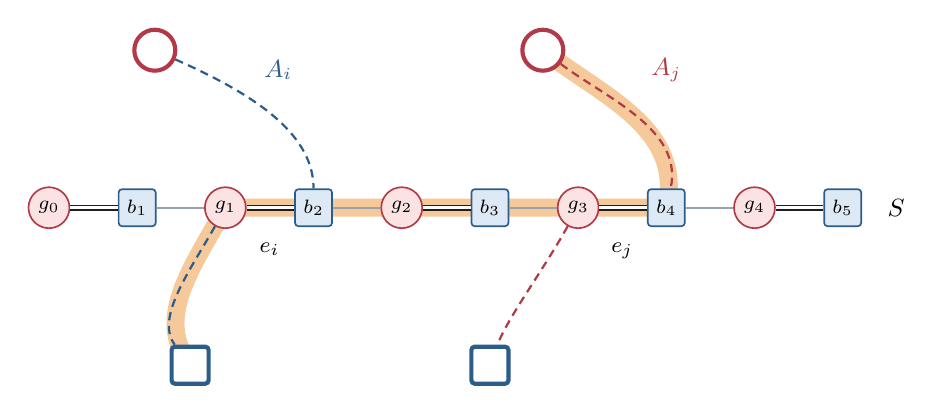
\begin{tikzpicture}[x=1.12cm,y=1cm]
% P after augmentation: g0 b1 g1 b2 g2 b3 g3 b4 g4 b5, couples g_{k-1} b_k
\foreach \lab/\x in {g_0/0,g_1/2,g_2/4,g_3/6,g_4/8}{\node[girl] (\lab) at (\x,0) {$\lab$};}
\foreach \lab/\x in {b_1/1,b_2/3,b_3/5,b_4/7,b_5/9}{\node[boy] (\lab) at (\x,0) {$\lab$};}
% free girls / boys of Q_i and Q_j
\node[girl,free] (qi0) at (1.2,2.0) {};
\node[boy,free]  (qi1) at (1.6,-2.0) {};
\node[girl,free] (qj0) at (5.6,2.0) {};
\node[boy,free]  (qj1) at (5.0,-2.0) {};
\begin{scope}[on background layer]
  % the spliced path
  \draw[sap] (qj0.center) .. controls (6.3,1.4) and (7.2,1.0) .. (b_4.center)
     -- (g_3.center) -- (b_3.center) -- (g_2.center) -- (b_2.center) -- (g_1.center)
     .. controls (1.6,-.8) and (1.2,-1.4) .. (qi1.center);
\end{scope}
% couples e_k of the new matching along P
\draw[couple] (g_0)--(b_1) (g_1)--(b_2) (g_2)--(b_3) (g_3)--(b_4) (g_4)--(b_5);
\draw[edge,line width=.75pt] (b_1)--(g_1) (b_2)--(g_2) (b_3)--(g_3) (b_4)--(g_4);
% Q_i and Q_j (schematic)
\draw[boydraw,line width=.8pt,densely dashed] (qi0) .. controls (2.2,1.5) and (3,1.0) .. (b_2);
\draw[boydraw,line width=.8pt,densely dashed] (g_1) .. controls (1.6,-.8) and (1.2,-1.4) .. (qi1);
\draw[girldraw,line width=.8pt,densely dashed] (qj0) .. controls (6.3,1.4) and (7.2,1.0) .. (b_4);
\draw[girldraw,line width=.8pt,densely dashed] (g_3) .. controls (5.6,-.8) and (5.2,-1.4) .. (qj1);
\node[font=\small,boydraw] at (2.6,1.75) {$A_i$};
\node[font=\small,girldraw] at (7.0,1.75) {$A_j$};
\node[font=\footnotesize,anchor=north] at (2.5,-.32) {$e_i$};
\node[font=\footnotesize,anchor=north] at (6.5,-.32) {$e_j$};
\node[font=\small,anchor=west] at (9.4,0) {$S$};
\end{tikzpicture}

\caption{Step~4 of the proof of Theorem~U. After augmenting along the
selected path $S$, its couples are the edges $e_k$ from $g_{k-1}$ to $b_k$.
If two disjoint augmenting paths $A_i$ and $A_j$ cross $S$ at $e_i$ and
$e_j$, the shaded splice is an augmenting path with $4(j-i)$ more edges
than either of them.}
\label{fig:splice}
\end{figure}

The splice argument also shows that a full set of disjoint new SAPs can
coexist with much longer augmenting paths.

\begin{proposition}
\label{prop:longpaths}
In the situation of Theorem~U, drop the hypothesis that all augmenting
paths for $M''$ have level~$L+1$, and assume only that its SAPs have level
$L+1$. If $M''$ has $q$ vertex-disjoint SAPs, each meeting a selected
path, then $M''$ has an augmenting path with at least
$2L+1+4(\ceil{q/a}-1)$ edges.
\end{proposition}

\begin{proof}
Steps~1 and~2 apply to SAPs. Some selected path $S$ meets at least
$k=\ceil{q/a}$ of the $q$ SAPs. Choose a shortest interval $[i,j]$ of
indices such that the couples $e_i,\ldots,e_j$ of $S$ include contacts with
all $k$ of them. The SAPs owning $e_i$ and $e_j$ have no other contact
inside the interval (otherwise it could be shortened), and $j-i\ge k-1$.
Splice as in Step~4; contacts with other SAPs inside the interval do no
harm, because those paths are not used.
\end{proof}

For example, in the first dag round of Knuth's 16-pair graph three SAPs
are selected, and the next matrix has five disjoint SAPs of level~3, each
meeting a selected one. So the second matching has an augmenting path
with at least $5+4=9$ edges, that is, of level at least~5; the census in
Appendix~\ref{app:knuth16} shows six of them.

\subsection{Consequences}

\begin{corollary}
If property $\Up$ holds in consecutive rounds at levels~$L,L+1,\ldots$,
and the first of them starts with $f>0$ free girls, there are at most
$\floor{\lg f}+1$ such rounds. The bound is attained when $f=1,2,4,8,16,32$,
and we expect it to be attained for every power of~2.
\end{corollary}

\begin{proof}
By Theorem~U every round except the last leaves at most $\floor{f/2}$ free
girls. Appendix~\ref{app:halving} describes ordered graphs, one for each
$f=2^t$, on which Algorithm~H halves the number of free girls in every
round while every augmenting path has the current shortest level
(Fig.~\ref{fig:halving}). For $f\le32$ we verified this by running
Algorithm~H and enumerating all augmenting paths in every round; the
appendix explains why it should hold in general, but we have not written
out a complete proof.
\end{proof}

\begin{figure}[ht]
\centering
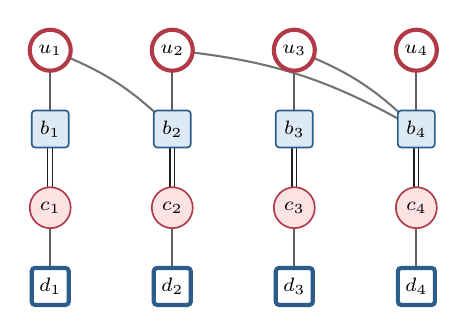
\begin{tikzpicture}[]
\draw[pedge] (3.100,1.500) -- (3.100,0.500);
\draw[edge,draw=black!55,line width=.75pt] (3.100,1.500) to[bend left=12] (4.650,0.500);
\draw[pedge] (0.000,1.500) -- (0.000,0.500);
\draw[edge,draw=black!55,line width=.75pt] (0.000,1.500) to[bend left=12] (1.550,0.500);
\draw[pedge] (1.550,1.500) -- (1.550,0.500);
\draw[edge,draw=black!55,line width=.75pt] (1.550,1.500) to[bend left=12] (4.650,0.500);
\draw[pedge] (4.650,1.500) -- (4.650,0.500);
\draw[couple] (0.000,-0.500) -- (0.000,0.500);
\draw[pedge] (0.000,-0.500) -- (0.000,-1.500);
\draw[couple] (1.550,-0.500) -- (1.550,0.500);
\draw[pedge] (1.550,-0.500) -- (1.550,-1.500);
\draw[couple] (3.100,-0.500) -- (3.100,0.500);
\draw[pedge] (3.100,-0.500) -- (3.100,-1.500);
\draw[couple] (4.650,-0.500) -- (4.650,0.500);
\draw[pedge] (4.650,-0.500) -- (4.650,-1.500);
\node[girl,free] at (0.000,1.500) {$u_{1}$};
\node[boy] at (0.000,0.500) {$b_{1}$};
\node[girl] at (0.000,-0.500) {$c_{1}$};
\node[boy,free] at (0.000,-1.500) {$d_{1}$};
\node[girl,free] at (1.550,1.500) {$u_{2}$};
\node[boy] at (1.550,0.500) {$b_{2}$};
\node[girl] at (1.550,-0.500) {$c_{2}$};
\node[boy,free] at (1.550,-1.500) {$d_{2}$};
\node[girl,free] at (3.100,1.500) {$u_{3}$};
\node[boy] at (3.100,0.500) {$b_{3}$};
\node[girl] at (3.100,-0.500) {$c_{3}$};
\node[boy,free] at (3.100,-1.500) {$d_{3}$};
\node[girl,free] at (4.650,1.500) {$u_{4}$};
\node[boy] at (4.650,0.500) {$b_{4}$};
\node[girl] at (4.650,-0.500) {$c_{4}$};
\node[boy,free] at (4.650,-1.500) {$d_{4}$};
\end{tikzpicture}

\caption{The halving graph for $f=4$ ($s=8$), with the matching after~\Hs1.
Free girl~$u_i$ is adjacent to $b_i$ and, if $i<4$, also to $b_{i+2^{\rho(i)}}$,
where $2^{\rho(i)}$ is the largest power of~2 dividing~$i$. Each dag round
merges pairs of neighbouring groups of indices (Appendix~\ref{app:halving}),
and the free girls go $4\to2\to1\to0$. At every stage all augmenting paths
have the same level.}
\label{fig:halving}
\end{figure}

\begin{lthm}[Corollary]{L}
For $s\ge1$, a literal realization of the Tchoukaillon schedule exists
if and only if $s\in\{1,2,3,4,5,8,9\}$.
\end{lthm}

\begin{proof}
The schedule starts with $f=\floor{s/2}$ free girls at level~2 and removes
$a=\ceil{f/3}$ SAPs. If any girls remain, the next round is at level~3 and,
in a literal realization, has property $\Up$; then Theorem~U requires
$f\le2\ceil{f/3}$. This fails for $f=3$ and for every $f\ge5$, which
excludes $s=6,7$ and all $s\ge10$.

For $s=2,4,8$, take the halving graphs with $f=1,2,4$: their free girls go
$1\to0$, $2\to1\to0$, and $4\to2\to1\to0$, which is the schedule in these
cases. For $s=3,5,9$, add one isolated girl--boy edge, numbered last;
\Hs1 matches it and nothing else changes, and $\floor{s/2}$ is unchanged.
For $s=1$ a single edge will do.
\end{proof}

So Knuth's 16-pair graph cannot be repaired into a literal example: no
graph and no input order satisfy the literal definition at $s=16$. Nothing
in this section obstructs the basic-row or operational readings, and
Knuth's graph meets the basic-row reading at $s=16$.

\section{The operational question}
\label{sec:operational}

Can every $s$ be given an ordered graph that realizes the Tchoukaillon
schedule, with no condition on the paths? This is exercise~16 under the
operational reading, and it is open. This section collects what we know:
explicit examples for small $s$, an example showing that the operational
and basic-row readings differ, structural consequences of the
schedule's first rounds, and two obstructions that come from the input
order.

\subsection{Small sizes}
\label{sec:catalog}

An earlier computer search found ordered graphs realizing the schedule for
every even $s\le40$ (Appendix~\ref{app:catalog}). It extended one fixed
ordered graph step by step, rerunning the whole execution after each
proposed extension and rejecting any extension that changed an earlier
round. Its program is not among the accompanying programs, but the inputs
it found are. The program \texttt{search.py} (Appendix~\ref{app:code}) is a
new search of the same kind. It finds other graphs, for every even
$s\le46$ with its default seed and, with other seeds, also for $s=48$, 52,
54, and~56. With Proposition~\ref{prop:pad} for $s=50$ and the next
proposition for odd~$s$, the schedule can therefore be realized for every
$s\le57$. It starts from the normal form of Appendix~\ref{app:catalog} and
designs one round at a time, in the manner of Knuth's matrices
(answer~15(d)): at level~$L$ it splits the rows into groups of at most
$L+1$, and for each group it adds the edges of one SAP that merges the
group's rows, placed in the lists so that Algorithm~H should find exactly
that SAP. After each proposed group it reruns the whole execution
from~\Hs1, and it rejects the group if an earlier round changes or the
planned SAPs are not found. Neither search is guaranteed to succeed
(with its default seed \texttt{search.py} finds nothing for $s=48$, 50,
or~52 in two minutes each, and five other seeds found nothing for $s=58$, 60,
or~62 in fifteen minutes each), and neither proves anything about
larger~$s$. We have replayed every
example from both searches from \Hs1 with two independent implementations
of Algorithm~H and checked its final matching with a separate
maximum-matching program (Appendix~\ref{app:code}). A max-flow computation
of $\nu$ in every round shows that all these examples are in fact basic-row
realizations.

\begin{proposition}
\label{prop:odd}
A realization for $s=2h$ yields one for $s=2h+1$: add an isolated
girl--boy edge, numbered after all other vertices. The new realization is
basic-row if the old one is.
\end{proposition}

\begin{proof}
\Hs1 matches the new edge first, no search ever reaches it, and
$\floor{2h/2}=\floor{(2h+1)/2}$, so the schedule is unchanged.
\end{proof}

\subsection{Operational is weaker than basic-row}
\label{sec:no-cover}

The matrices of answer~15(d) keep $\nu=f$ in every round
(property~$\Bp$). The schedule does not require this. Take $s=8$ and the
ordered lists
\begin{equation}
  [5,7];\ [3,5];\ [3];\ [1];\ [1,2];\ [3,4];\ [5,2,6];\ [7,8].
  \label{eq:tree8}
\end{equation}
The graph is a tree with 15 edges (Fig.~\ref{fig:tree8}). Step~\Hs1 leaves
girls~$4,3,2,1$ free, and the run is
\begin{center}\small
\begin{tabular}{crrrrr}
\toprule
$L$&$f$&SAPs&$W_5$&$W_{13}$&$W_{11}$\\
\midrule
2&4&2&15&7&8\\
3&2&1&11&3&5\\
4&1&1&7&4&4\\
\bottomrule
\end{tabular}
\end{center}
which is the schedule $4\to2\to1\to0$. After the round at level~2 (round~2
of the run), the free girls are $g_3,g_4$ and the free boys~$b_6,b_8$, and
there are exactly three augmenting paths,
\begin{align*}
 &g_4\sg b_1\db g_5\sg b_2\db g_7\sg b_6 &&(\text{level }3),\\
 &g_3\sg b_3\db g_2\sg b_5\db g_1\sg b_7\db g_8\sg b_8 &&(\text{level }4),\\
 &g_4\sg b_1\db g_5\sg b_2\db g_7\sg b_5\db g_1\sg b_7\db g_8\sg b_8 &&(\text{level }5).
\end{align*}
(In a tree there is at most one path between two vertices, so one only
has to check the four pairs of a free girl and a free boy.) So with two
free girls there is only one SAP, $\nu=1<f$, and property~$\Bp$ fails for
every choice of perfect matching. An operational realization need not be
basic-row, and a search restricted to Knuth-style matrices could miss
solutions.

\begin{figure}[ht]
\centering
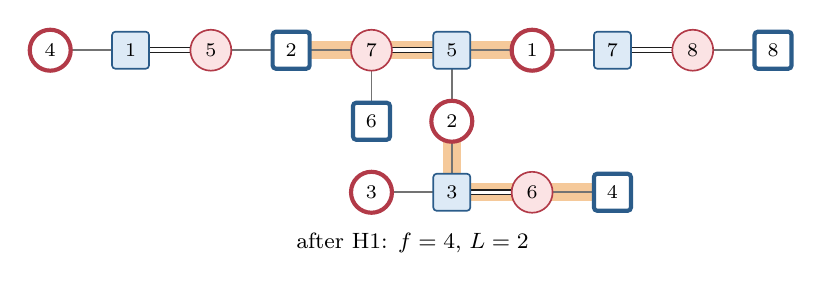
\begin{tikzpicture}[]
\begin{scope}[on background layer]
\draw[sap] (6.120,0.000) -- (5.100,0.000) -- (4.080,0.000) -- (3.060,0.000);
\draw[sap] (5.100,-0.902) -- (5.100,-1.804) -- (6.120,-1.804) -- (7.140,-1.804);
\end{scope}
\draw[edge,draw=black!55,line width=.7pt] (6.120,0.000) -- (5.100,0.000);
\draw[edge,draw=black!55,line width=.7pt] (6.120,0.000) -- (7.140,0.000);
\draw[edge,draw=black!55,line width=.7pt] (5.100,-0.902) -- (5.100,-1.804);
\draw[edge,draw=black!55,line width=.7pt] (5.100,-0.902) -- (5.100,0.000);
\draw[edge,draw=black!55,line width=.7pt] (4.080,-1.804) -- (5.100,-1.804);
\draw[edge,draw=black!55,line width=.7pt] (0.000,0.000) -- (1.020,0.000);
\draw[couple] (2.040,0.000) -- (1.020,0.000);
\draw[edge,draw=black!55,line width=.7pt] (2.040,0.000) -- (3.060,0.000);
\draw[couple] (6.120,-1.804) -- (5.100,-1.804);
\draw[edge,draw=black!55,line width=.7pt] (6.120,-1.804) -- (7.140,-1.804);
\draw[couple] (4.080,0.000) -- (5.100,0.000);
\draw[edge,draw=black!55,line width=.7pt] (4.080,0.000) -- (3.060,0.000);
\draw[edge,draw=black!55,line width=.7pt] (4.080,0.000) -- (4.080,-0.902);
\draw[couple] (8.160,0.000) -- (7.140,0.000);
\draw[edge,draw=black!55,line width=.7pt] (8.160,0.000) -- (9.180,0.000);
\node[girl,free] at (0.000,0.000) {4};
\node[girl] at (2.040,0.000) {5};
\node[girl] at (4.080,0.000) {7};
\node[girl,free] at (6.120,0.000) {1};
\node[girl] at (8.160,0.000) {8};
\node[girl,free] at (5.100,-0.902) {2};
\node[girl,free] at (4.080,-1.804) {3};
\node[girl] at (6.120,-1.804) {6};
\node[boy] at (1.020,0.000) {1};
\node[boy,free] at (3.060,0.000) {2};
\node[boy] at (5.100,0.000) {5};
\node[boy] at (7.140,0.000) {7};
\node[boy,free] at (9.180,0.000) {8};
\node[boy,free] at (4.080,-0.902) {6};
\node[boy] at (5.100,-1.804) {3};
\node[boy,free] at (7.140,-1.804) {4};
\node[font=\footnotesize] at (4.6,-2.45) {after \Hs1: $f=4$, $L=2$};
\end{tikzpicture}

\bigskip

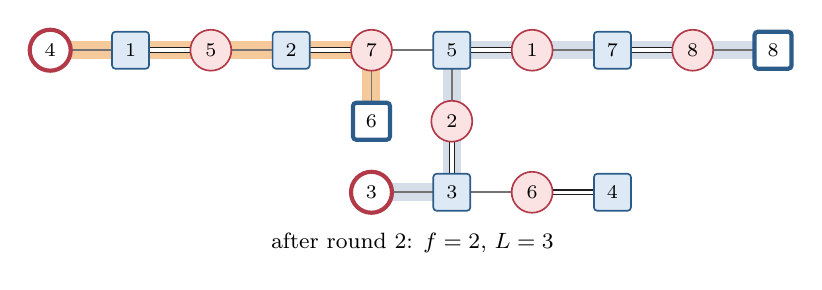
\begin{tikzpicture}[]
\begin{scope}[on background layer]
\draw[sap] (0.000,0.000) -- (1.020,0.000) -- (2.040,0.000) -- (3.060,0.000) -- (4.080,0.000) -- (4.080,-0.902);
\draw[sap,draw=boydraw,opacity=.2] (4.080,-1.804) -- (5.100,-1.804) -- (5.100,-0.902) -- (5.100,0.000) -- (6.120,0.000) -- (7.140,0.000) -- (8.160,0.000) -- (9.180,0.000);
\end{scope}
\draw[couple] (6.120,0.000) -- (5.100,0.000);
\draw[edge,draw=black!55,line width=.7pt] (6.120,0.000) -- (7.140,0.000);
\draw[couple] (5.100,-0.902) -- (5.100,-1.804);
\draw[edge,draw=black!55,line width=.7pt] (5.100,-0.902) -- (5.100,0.000);
\draw[edge,draw=black!55,line width=.7pt] (4.080,-1.804) -- (5.100,-1.804);
\draw[edge,draw=black!55,line width=.7pt] (0.000,0.000) -- (1.020,0.000);
\draw[couple] (2.040,0.000) -- (1.020,0.000);
\draw[edge,draw=black!55,line width=.7pt] (2.040,0.000) -- (3.060,0.000);
\draw[edge,draw=black!55,line width=.7pt] (6.120,-1.804) -- (5.100,-1.804);
\draw[couple] (6.120,-1.804) -- (7.140,-1.804);
\draw[edge,draw=black!55,line width=.7pt] (4.080,0.000) -- (5.100,0.000);
\draw[couple] (4.080,0.000) -- (3.060,0.000);
\draw[edge,draw=black!55,line width=.7pt] (4.080,0.000) -- (4.080,-0.902);
\draw[couple] (8.160,0.000) -- (7.140,0.000);
\draw[edge,draw=black!55,line width=.7pt] (8.160,0.000) -- (9.180,0.000);
\node[girl,free] at (0.000,0.000) {4};
\node[girl] at (2.040,0.000) {5};
\node[girl] at (4.080,0.000) {7};
\node[girl] at (6.120,0.000) {1};
\node[girl] at (8.160,0.000) {8};
\node[girl] at (5.100,-0.902) {2};
\node[girl,free] at (4.080,-1.804) {3};
\node[girl] at (6.120,-1.804) {6};
\node[boy] at (1.020,0.000) {1};
\node[boy] at (3.060,0.000) {2};
\node[boy] at (5.100,0.000) {5};
\node[boy] at (7.140,0.000) {7};
\node[boy,free] at (9.180,0.000) {8};
\node[boy,free] at (4.080,-0.902) {6};
\node[boy] at (5.100,-1.804) {3};
\node[boy] at (7.140,-1.804) {4};
\node[font=\footnotesize] at (4.6,-2.45) {after round 2: $f=2$, $L=3$};
\end{tikzpicture}

\caption{An operational realization for $s=8$ that is not basic-row,
labelled by the numbers of~\eqref{eq:tree8}. Top: the matching after~\Hs1
and the two SAPs of the round at level~2. Bottom: the next matching. Its
only SAP is shaded orange; the faint blue path is the augmenting path of
level~4. (The third augmenting path, of level~5, is not drawn.)}
\label{fig:tree8}
\end{figure}

\subsection{The shape forced by the first matching}
\label{sec:blocks}

For even $s=2h$ the schedule asks~\Hs1 to leave $h$ girls free, so~\Hs1 must
produce a maximal matching with only $h$ couples, the fewest possible. The
next proposition describes what that implies for the graph, whatever the
input order. Write $G^\circ$ and $G^\bullet$ for the girls who are free and
matched after~\Hs1, and $B^\bullet$ and $B^\circ$ for the boys who are
matched and free after~\Hs1.

\begin{proposition}
\label{prop:blocks}
Suppose $s=M=N=2h$ and~\Hs1 leaves $h$ girls free. Then:
\begin{enumerate}[label=(\alph*)]
\item there are no edges between $G^\circ$ and $B^\circ$, so the biadjacency
  matrix has the block form of Fig.~\ref{fig:blocks};
\item every perfect matching pairs $G^\circ$ with $B^\bullet$ and $G^\bullet$
  with $B^\circ$;
\item whenever $f$ girls are free later on, exactly $f$ couples join
  $G^\bullet$ to $B^\bullet$, and $h-f$ couples are of each of the types
  $G^\circ$--$B^\bullet$ and $G^\bullet$--$B^\circ$;
\item relative to any perfect matching, every basic path contains exactly
  one couple of type $G^\bullet$--$B^\bullet$.
\end{enumerate}
\end{proposition}

\begin{proof}
(a) is maximality of the matching from~\Hs1. For (b), the $h$ girls of
$G^\circ$ can only be matched into the $h$ boys of $B^\bullet$, which leaves
$B^\circ$ for $G^\bullet$. (c) Vertices never become free again once
matched, so $G^\bullet$ and $B^\bullet$ stay covered. If $x,y,z$ count the
current couples of types $G^\circ$--$B^\bullet$, $G^\bullet$--$B^\bullet$,
$G^\bullet$--$B^\circ$, then $x+y=|B^\bullet|=h$, $y+z=|G^\bullet|=h$, and
$x+y+z=2h-f$; hence $y=f$. (d) A basic path starts at a free girl in
$G^\circ$ and ends at a free boy in $B^\circ$. Its perfect-matching edges
stay within $G^\circ\cup B^\bullet$ or within $G^\bullet\cup B^\circ$
by~(b), its couples of the two mixed types do too, and a couple of type
$G^\bullet$--$B^\bullet$ is the only way to pass from the first part to the
second; by~(a) there is no way back.
\end{proof}

\begin{figure}[ht]
\centering
% Adjacency blocks after a minimum H1 (rows: girls; columns: boys).
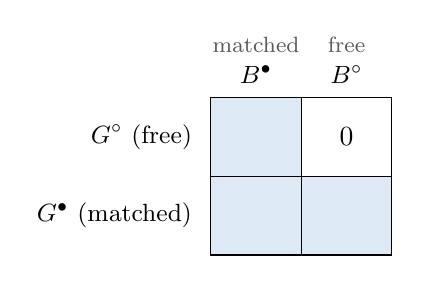
\begin{tikzpicture}[x=1.15cm,y=1.0cm]
\draw[fill=boyfill] (0,0) rectangle (1,1);
\draw[fill=white] (1,0) rectangle (2,1);
\draw[fill=boyfill] (0,-1) rectangle (1,0);
\draw[fill=boyfill] (1,-1) rectangle (2,0);
\node at (1.5,.5) {$0$};
\node[font=\small,anchor=east] at (-.1,.5) {$G^\circ$ (free)};
\node[font=\small,anchor=east] at (-.1,-.5) {$G^\bullet$ (matched)};
\node[font=\small,anchor=south] at (.5,1.05) {$B^\bullet$};
\node[font=\small,anchor=south] at (1.5,1.05) {$B^\circ$};
\node[font=\footnotesize,anchor=south,text=black!65] at (.5,1.45) {matched};
\node[font=\footnotesize,anchor=south,text=black!65] at (1.5,1.45) {free};
\end{tikzpicture}

\caption{After a minimum-size~\Hs1 matching no free girl is adjacent to a
free boy: the biadjacency matrix has a zero block.}
\label{fig:blocks}
\end{figure}

In terms of Knuth's matrices, each row consists of some indices of
initially free girls followed by some indices of initially matched girls.
For the 16-pair example this is the remark at the end of answer~15(d):
an edge $b_{\rm even}\sg g_{\rm odd}$ would join a free girl to a free boy
of the first matching.

\subsection{Realizations need cycles}

The trees of Section~\ref{sec:sparse} already force Algorithm~H to do
$\Theta(E\sqrt V)$ work. No forest, however, can realize the schedule for
large $s$: its first two rounds force many independent cycles. The
argument uses only the prescribed numbers of SAPs in those rounds, so it
applies to any algorithm that removes a maximal set of disjoint SAPs per
round, in any order.

\begin{lthm}{C}
Let an ordered graph with $s=M=N=2h>0$ realize the Tchoukaillon schedule.
Let $a_2=\ceil{h/3}$ and $a_3=\ceil{(h-a_2)/4}$ be the numbers of SAPs in
its rounds at levels~2 and~3, and let $p=3a_2-h\in\{0,1,2\}$. Then
\[
   E\ \ge\ 3h+4a_2-8p-a_3 .
\]
Consequently the cycle rank $\beta=E-V+\kappa$, where $\kappa$ is the number
of connected components, satisfies $\beta\ge a_2-a_3-7p+1\ge\ceil{(h-76)/6}$.
In particular the graph is not a forest if $h\ge77$, or if $3\mid h$; and for
large $s$,
\[
   E\ge\tfrac{25}{12}\,s-O(1),\qquad \beta\ge\tfrac1{12}\,s-O(1).
\]
\end{lthm}

\begin{proof}
Fix a perfect matching $P$ and let $M_1$ be the matching produced by~\Hs1.

\emph{Basic paths after~\Hs1.} The $2h$ endpoints of $M_1$ must touch all
$2h$ edges of $P$, by maximality, so each edge of $P$ has exactly one
matched endpoint. Hence $P\cup M_1$ is a disjoint union of $h$ basic paths
of level~2, each of the form $u\sg v\db w\sg z$ with $u\in G^\circ$, $v\in
B^\bullet$, $w\in G^\bullet$, $z\in B^\circ$; together they cover all
vertices and use $3h$ edges.

\emph{Good triples.} A SAP of the first dag round also has the form
$u\sg v\db w\sg z$, and it meets at most three basic paths: the one
containing~$u$, the one containing the couple $v\db w$, and the one
containing~$z$. The round selects $a_2$ SAPs, and by maximality they meet
all $h$ basic paths. Call a selected SAP \emph{good} if it meets three basic
paths that no other selected SAP meets. If $q_1,\ldots,q_{a_2}$ are the
numbers of basic paths met by the selected SAPs, put
$\delta=3a_2-\sum q_i\ge0$ and $\omega=\sum q_i-h\ge0$, so that
$\delta+\omega=p$. At most $\delta$ selected SAPs meet fewer than three
paths; and a basic path met by $k\ge2$ selected SAPs contributes $k-1$ to
$\omega$ and involves at most $k\le2(k-1)$ of them. So the number $g$ of
good SAPs satisfies $g\ge a_2-2p$.

\emph{What a good triple becomes.} Number the three basic paths met by a good
SAP as $u_k\sg v_k\db w_k\sg z_k$ ($k=1,2,3$), so that the SAP is
$u_1\sg v_2\db w_2\sg z_3$. After augmenting, the six pairs of the triple
form two basic paths of level~3 (Fig.~\ref{fig:goodtriple}):
\[
  u_2\sg v_2\db u_1\sg v_1\db w_1\sg z_1\qquad\text{and}\qquad
  u_3\sg v_3\db w_3\sg z_3\db w_2\sg z_2 .
\]
These are SAPs of the round at level~3, and their vertices lie in the dag
at the levels given by their positions (a shorter route to one of them,
followed by the rest of the path, would contain an augmenting path of
level~2, and there is none after the first dag round). The triple contains
$9+2=11$ edges of $P\cup M_1$ and of the selected SAP: the ten edges of the
two new paths, and the old couple $v_2w_2$. That edge joins the girl~$w_2$,
at position~3 of the second path, to the boy~$v_2$, at position~1 of the
first, so it points backwards and is not an arc of the level-3 dag.

\emph{The second round.} Let $F$ be the set of edges outside $P\cup M_1$ and
outside the $2g$ selected edges of good triples; $|F|=E-3h-2g$. In the
level-3 dag with $F$ removed, each new path of a good triple is cut off
from everything else: edges of $P\cup M_1$ never leave their triple, the
selected edges stay inside it, and the only remaining edge between the two
new paths is not an arc. So a SAP that meets $q$ of these $2g$ paths uses at
least $q-1$ edges of~$F$. The round at level~3 selects $a_3$ vertex-disjoint
SAPs, which must meet all $2g$ new paths of good triples. Therefore
$2g-a_3\le|F|=E-3h-2g$, and $E\ge3h+4g-a_3\ge3h+4a_2-8p-a_3$.

(When $h=1$ there is no second round, $a_3=0$, and the bound is trivial.)
The bound on $\beta$ follows from $V=4h$, $\kappa\ge1$, and $h=3a_2-p$; the
explicit form comes from substituting $a_3=\ceil{(2a_2-p)/4}$ and checking
$p=0,1,2$, the weakest case being $p=2$ with $a_2$ even. For $p=0$ one gets
$\beta\ge\floor{a_2/2}+1>0$. The asymptotic statements follow from
$a_2=h/3+O(1)$ and $a_3=h/6+O(1)$.
\end{proof}

\begin{figure}[ht]
\centering
% A good triple (proof of Theorem C): before and after the first dag round.
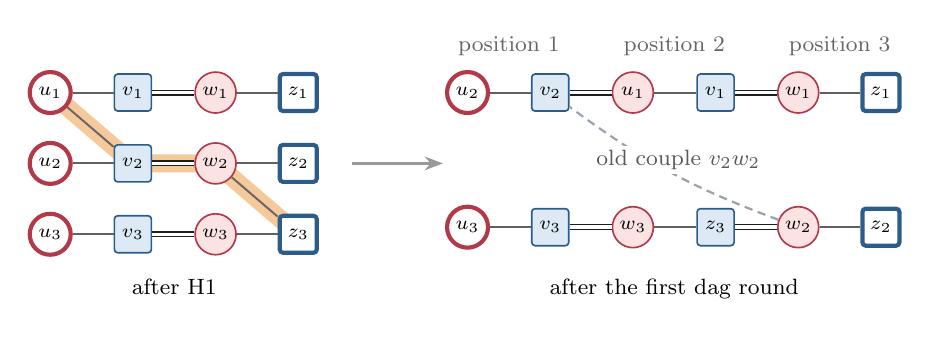
\begin{tikzpicture}[x=1.05cm,y=.9cm]
% ---------- left: three basic paths after H1, one selected SAP
\foreach \k/\y in {1/0,2/-1,3/-2}{
  \node[girl,free] (u\k) at (0,\y) {$u_\k$};
  \node[boy]       (v\k) at (1,\y) {$v_\k$};
  \node[girl]      (w\k) at (2,\y) {$w_\k$};
  \node[boy,free]  (z\k) at (3,\y) {$z_\k$};
  \draw[pedge] (u\k)--(v\k) (w\k)--(z\k);
  \draw[couple] (v\k)--(w\k);}
\begin{scope}[on background layer]
  \draw[sap] (u1.center)--(v2.center)--(w2.center)--(z3.center);
\end{scope}
\draw[edge,draw=black!60,line width=.7pt] (u1)--(v2) (w2)--(z3);
\node[font=\footnotesize,anchor=north] at (1.5,-2.5) {after \Hs1};
% ---------- right: the two new basic paths
\begin{scope}[xshift=5.3cm]
  \foreach \p in {1,2,3}{\node[font=\footnotesize,text=black!60] at ({2*\p-1.5},.65) {position \p};}
  \node[girl,free] (nu2) at (0,0) {$u_2$};
  \node[boy]       (nv2) at (1,0) {$v_2$};
  \node[girl]      (nu1) at (2,0) {$u_1$};
  \node[boy]       (nv1) at (3,0) {$v_1$};
  \node[girl]      (nw1) at (4,0) {$w_1$};
  \node[boy,free]  (nz1) at (5,0) {$z_1$};
  \node[girl,free] (nu3) at (0,-1.9) {$u_3$};
  \node[boy]       (nv3) at (1,-1.9) {$v_3$};
  \node[girl]      (nw3) at (2,-1.9) {$w_3$};
  \node[boy]       (nz3) at (3,-1.9) {$z_3$};
  \node[girl]      (nw2) at (4,-1.9) {$w_2$};
  \node[boy,free]  (nz2) at (5,-1.9) {$z_2$};
  \draw[pedge] (nu2)--(nv2) (nu1)--(nv1) (nw1)--(nz1) (nu3)--(nv3) (nw3)--(nz3) (nw2)--(nz2);
  \draw[couple] (nv2)--(nu1) (nv1)--(nw1) (nv3)--(nw3) (nz3)--(nw2);
  \draw[edgecol,line width=.8pt,densely dashed] (nw2) to[bend left=8] (nv2);
  \node[font=\footnotesize,text=black!65,fill=white,inner sep=1.5pt] at (2.55,-.95) {old couple $v_2w_2$};
  \node[font=\footnotesize,anchor=north] at (2.5,-2.5) {after the first dag round};
\end{scope}
\draw[-{Stealth},black!40,line width=.8pt] (3.65,-1)--(4.75,-1);
\end{tikzpicture}

\caption{A good triple in the proof of Theorem~C. Single lines are edges of
the perfect matching $P$, double lines are couples. One SAP of the first
dag round (shaded) meets three basic paths; afterwards their six pairs form
two basic paths of level~3. The old couple $v_2w_2$ runs from position~3
back to position~1, so the level-3 dag cannot use it, and any SAP that
visits both new paths must use some other edge.}
\label{fig:goodtriple}
\end{figure}

\begin{remark}
For odd $s=2h+1$ the same method should give
$E\ge3h+4a_2-8p-a_3-6$ and $\beta\ge\ceil{(h-124)/6}$, so that no forest
realizes the schedule when $s\ge251$. In outline: \Hs1 now leaves $h$ girls
free, and either all $h$ basic paths have level~2 and one couple of $M_1$
belongs to $P$, or one basic path has level~3 and the others level~2. We
have not written out the second case in full (one must check that SAPs
touching the long basic path do not spoil the isolation argument), so we
state this only as a remark.
\end{remark}

The case~$p=0$ also shows how property~$\Up$ fails in such a realization.

\begin{corollary}
If a realization has $6\mid s$, then just after its first dag round the
SAPs have level~3 (five edges), and there is also an augmenting path with
at least nine edges.
\end{corollary}

\begin{proof}
With $p=0$ all $a_2$ selected SAPs are good, so no basic path is left
untouched, and the $2a_2$ new basic paths are disjoint SAPs of level~3,
each meeting a selected SAP. Apply Proposition~\ref{prop:longpaths} with
$q=2a_2$ and $a=a_2$.
\end{proof}

\subsection{The input order matters}
\label{sec:order}

One plan for the operational question is to find a graph with the right
sequence of maximal SAP sets, and then look for an input order that makes
Algorithm~H pick those sets. The plan can fail, because Algorithm~H does
not choose its maximal sets freely: which SAP it finds depends on the
order in \A{QUEUE}, on head insertion in step~\Hs6, and on the replacement
rule of step~\Hs{16}.

\paragraph{A six-pair graph.}
Let the girls~$g_1,\ldots,g_6$ have the neighbour sets
\[
  \{b_1\};\quad\{b_1,b_2,b_5\};\quad\{b_3\};\quad\{b_2,b_3,b_4\};\quad\{b_3,b_5\};\quad\{b_5,b_6\}.
\]
The edges $g_kb_k$ form a perfect matching. Starting from the matching
$b_1g_2$, $b_3g_4$, $b_5g_6$, the three augmentations
\begin{gather*}
  g_5\sg b_3\db g_4\sg b_2,\qquad
  g_1\sg b_1\db g_2\sg b_5\db g_6\sg b_6,\\
  g_3\sg b_3\db g_5\sg b_5\db g_2\sg b_2\db g_4\sg b_4
\end{gather*}
are SAPs at levels~2, 3, 4, and after each of them no SAP of the same level
remains. So the schedule for $s=6$, which removes one SAP at each of these
levels, is consistent with this graph.

\begin{proposition}
No numbering and no list order make Algorithm~H follow this schedule on
this graph.
\end{proposition}

\begin{proof}
A maximal matching with three couples must have exactly one endpoint on
each edge $g_kb_k$ and contain none of them; the only such matching is
$b_1g_2$, $b_3g_4$, $b_5g_6$, so~\Hs1 must produce it, with free girls
$g_1,g_3,g_5$. One SAP can be a maximal set only if it meets all three
basic paths, and the only such SAP is $g_5\sg b_3\db g_4\sg b_2$. Before
the first augmentation every root of the search succeeds, so this must be
the SAP found from the first root, $b_2$, by taking the first arc of each
list. Head insertion at $b_3$ then requires $g_3$ to precede $g_5$ in
\A{QUEUE}, and head insertion at $b_2$ requires $g_2$ to precede $g_4$ at
level~1. Girl~$g_2$ is queued when $g_1$ discovers $b_1$, and $g_4$ when the
earlier of $g_3,g_5$ discovers $b_3$; so $g_1$ comes first, and the queue
must be $(g_1,g_3,g_5)$. Step~\Hs{16} then removes the last girl, $g_5$,
leaving $(g_1,g_3)$. In the next dag, level~1 is $(g_2,g_5)$, both adjacent
to $b_5$, so $\A{BLINK}[b_5]=(g_5,g_2)$ whatever the lists. Whichever of the
free boys~$b_4,b_6$ is searched first finds one of the basic paths
$g_1\sg b_1\db g_2\sg b_2\db g_4\sg b_4$ or $g_3\sg b_3\db g_5\sg b_5\db
g_6\sg b_6$; they are disjoint, so the other is found as well, and the round
removes two SAPs instead of one.
\end{proof}

An exhaustive check of all $6!\,(3!)^2(2!)^2=103680$ girl numberings and
list orders (the boy numbering plays no role) agrees: 740 of them give a
three-couple~\Hs1 matching, and none of those follows the schedule. Other
six-pair graphs do realize it (Appendix~\ref{app:catalog}).

\paragraph{Triangular chain graphs.}
Let $\Delta_{2h}$ have girls and boys~$1,\ldots,2h$, with $g_j\sg b_i$ an
edge whenever $i\le j$. Hegerfeld and Kratsch show that chain graphs of
this kind can need many phases when the maximal sets are chosen
adversarially~\cite[Section~5.3]{HegerfeldKratsch}. With Algorithm~H and a
minimum-size first matching, the order of the search rules out the
Tchoukaillon schedule whenever $3\mid h$:

\begin{proposition}
\label{prop:chain}
Give $\Delta_{2h}$ any numbering and any list order. If~\Hs1 leaves $h$ girls
free and the first dag round finds $a$ SAPs, then $3a>h$. So when $3\mid h$,
the graph $\Delta_{2h}$ cannot realize the schedule, whose first round would
remove exactly $h/3$ SAPs.
\end{proposition}

\begin{proof}
As in the previous proof, each edge $g_kb_k$ has exactly one matched
endpoint. Let $T$ be the set of $k$ with $g_k$ free (so $b_k$ is matched)
and $S$ its complement (so $b_k$ is free). Maximality forbids an edge from a
free girl~$g_t$ to a free boy~$b_u$; since $g_tb_u$ is an edge when $u\le
t$, we must have $u>t$ for all $t\in T$ and $u\in S$. Hence
$T=\{1,\ldots,h\}$ and $S=\{h+1,\ldots,2h\}$. Write $u_i=g_i$, $v_i=b_i$,
$x_j=g_{h+j}$, $z_j=b_{h+j}$ for $1\le i,j\le h$; the matching from~\Hs1 is
$x_j\db v_{\pi(j)}$ for a permutation~$\pi$, and the SAPs are exactly the
paths
\[
   u_i\sg v_{\pi(j)}\db x_j\sg z_d\qquad\text{with }\pi(j)\le i\text{ and }d\le j .
\]
Suppose $a<h$ SAPs are selected, let $i_0$ be the largest index of an
unselected free girl and $d_0$ the smallest index of an unselected free boy.
An unselected $x_j$ with $\pi(j)\le i_0$ and $j\ge d_0$ would give a SAP
disjoint from the selected ones; so each of the $h-a$ unselected $x_j$ has
$\pi(j)>i_0$ or $j<d_0$. At most $h-i_0\le a$ of them satisfy the first
condition and at most $d_0-1\le a$ the second; hence $h\le3a$.

Suppose $h=3a$. Then all these inequalities are equalities: the selected
free girls are $u_{2a+1},\ldots,u_{3a}$, the selected free boys are
$z_1,\ldots,z_a$, every selected $x_j$ has $\pi(j)\le2a$ and $j>a$, and
every $x_j$ with $\pi(j)>2a$ is unselected and has $j>a$. Girl~$u_{2a}$ is
never selected. Each selected SAP passes through a boy~$v_{\pi(j)}$ with
$\pi(j)\le2a$, whose list contains $u_{2a}$; that arc cannot have been
consumed earlier, because following it would have produced a SAP ending at
$u_{2a}$. Since lists are in reverse queue order, every selected free girl
comes after $u_{2a}$ in \A{QUEUE}. Only the selected free girls are adjacent
to the boys~$v_{2a+1},\ldots,v_{3a}$, while $u_{2a}$ is adjacent to all of
$v_1,\ldots,v_{2a}$; so the latter are all discovered first, and their
mates come first in level~1. In particular every $x_j$ with $\pi(j)>2a$ is
queued after every selected $x_j$. Now consider the first root of the
search. Before any augmentation every root succeeds, so it is a selected
free boy~$z_d$ with $d\le a$. All $x_j$ with $\pi(j)>2a$ are adjacent to it
(since $j>a\ge d$) and come later in the queue, so the head of
$\A{BLINK}[z_d]$ is not a selected girl; and the search from it succeeds.
So the first SAP found uses an $x_j$ that should have remained unselected,
a contradiction.
\end{proof}

For $h=3$ the schedule is consistent with the graph itself: starting from
the matching $x_1v_1$, $x_2v_3$, $x_3v_2$, the graph $\Delta_6$ admits the
single maximal SAPs
\begin{gather*}
  u_3\sg v_2\db x_3\sg z_1,\qquad
  u_1\sg v_1\db x_1\sg z_1\db x_3\sg z_2,\\
  u_2\sg v_2\db u_3\sg v_3\db x_2\sg z_2\db x_3\sg z_3
\end{gather*}
at levels~$2,3,4$. It is the order of Algorithm~H's search that rules them
out. Other graphs with $s=6$ do realize the schedule.

\subsection{What an induction would need}

One might try to pass from $s=2h$ to $s=2h+2$ by adding two pairs. The
schedule changes in a very controlled way. Write $f_L(h)$ and $a_L(h)$ for
the schedule with $f_2(h)=h$, extended by zeros.

\begin{lemma}
\label{lem:step}
Let $K$ be the first level~$L\ge2$ such that $L+1$ divides $f_L(h)$. Then
$f_L(h+1)=f_L(h)+1$ for $2\le L\le K$ and $f_L(h+1)=f_L(h)$ for $L>K$; so
$a_L(h+1)=a_L(h)+\Iv{L=K}$.
\end{lemma}

\begin{proof}
The map $x\mapsto x-\ceil{x/(L+1)}$ increases by $1$ from $x$ to $x+1$,
except when $(L+1)\mid x$, where it stays the same. Start from a difference
of $1$ at level~2 and follow it.
\end{proof}

So adding two pairs should add one free girl, keep every count of SAPs
except one extra at level~$K$, and then rejoin the old schedule. When $K=2$,
that is, when $3\mid h$, this can be done.

\begin{proposition}
\label{prop:pad}
Let an ordered graph $G$ realize the schedule for $s=2h$, where $3\mid h$.
Let $q$ be the first girl in \A{QUEUE} after step~\Hs1, let $b$ be the first
boy on her list, and let $x$ be the girl whom~\Hs1 matches to~$b$. Form $G^+$
by adding girls $u$ and $w$, numbered below all girls of~$G$, boys $v$
and~$z$, the lists $u\colon[v]$ and $w\colon[v,z]$, and the edge $xz$, placed
in $x$'s list immediately after~$b$. Then $G^+$ realizes the schedule for
$s+2$, and it is basic-row if $G$ is.
\end{proposition}

\begin{proof}
Step~\Hs1 scans the girls of $G$ first and does what it did in~$G$: when $x$
is scanned, the boys before $b$ in her list are taken and $b$ is free, so
she never reaches~$z$. Then $w$ takes~$v$, and $u$ remains free. So
\A{QUEUE} is that of~$G$ followed by~$u$, with $h+1$ girls.

In the first dag, $q$ is scanned first. Her first boy $b$ is matched,
because $q$ is free after a maximal matching; so $b$ is the first boy of
level~1, and $x$ is the first girl of level~1. In her list, $x$ meets
matched boys (all taken by~\Hs1), then her mate~$b$, then $z$, who is free:
so $L=2$ and $z$ is the first root. The other free boys of level~2 are
entered in the same order as in~$G$, because only matched boys, which are
never roots, are treated differently once $L$ is known. Girl~$u$ is last at
level~0, so $w$ is last at level~1, and step~\Hs6 puts her at the head of
$\A{BLINK}[z]$. The search from~$z$ therefore takes~$w$ and then~$v$, whose
only girl at level~0 is~$u$: it finds the SAP $u\sg v\db w\sg z$. Since $u$
is the last free girl, step~\Hs{16} moves nobody. From then on the roots,
the lists \A{BLINK} of the boys of~$G$ (none of which contains a new girl),
and \A{QUEUE} are as in~$G$, so the round finds the $a_2(h)$ SAPs of~$G$ in
the same order, with the same moves in step~\Hs{16}. By
Lemma~\ref{lem:step} with $K=2$, that makes $a_2(h+1)$ SAPs, and after this
round the two schedules agree.

In later rounds $u$, $v$, $w$, $z$ are matched, and the only edge between them
and~$G$ is~$xz$. The breadth-first search may enter $z$, $w$, $v$, $u$
from~$x$, but they lead to no free boy, they do not change the relative
order of the vertices of~$G$ in \A{MARKED} or \A{QUEUE}, and no list
$\A{BLINK}[b']$ with $b'$ in~$G$ gains a girl. The depth-first search starts
at free boys of~$G$, and from a boy of~$G$ it reaches only girls of~$G$,
whose mates are boys of~$G$; so it never leaves~$G$. Every later round is
therefore the corresponding round of~$G$. Finally, in the first dag round
the $h$ disjoint SAPs of a basic-row~$G$ and the path $u\sg v\db w\sg z$
give $\nu=h+1=f$, and afterwards no augmenting path meets the new vertices.
\end{proof}

The edge $xz$ matters. Without it $z$ is the last root, the new SAP is found
last, and by then step~\Hs{16} may have moved~$u$ into the place of a girl
of~$G$, which changes the order of later searches; for $s=42$ and $s=54$
the padding then fails. For $K>2$ the extra free girl must survive several
rounds, and doing this with a fixed set of edges, while preserving every
earlier distance and every earlier \A{BLINK} order, is what we have not
managed: an edge added for a later round can create a shorter path in an
earlier one, or change the order in which an earlier search discovers
vertices.

\section{Simpler examples for the running time}
\label{sec:sparse}

If one only wants inputs on which Algorithm~H does $\Theta(E\sqrt V)$ work,
without the exact maximum number of rounds, a much simpler family will do.
It is the folklore example of disjoint paths with $3,5,7,\ldots$ edges, on
which every phase is forced (compare Hegerfeld and Kratsch's paths
\cite[Section~5.1]{HegerfeldKratsch}), here joined into a tree and given an
input order for Algorithm~H, with exact operation counts.

For $k=2,3,\ldots,K$ let $c_k=k(k-1)/2$ and form a path on the girls
$x_i=g_{c_k+i}$ and boys~$y_i=b_{c_k+i}$, $0\le i<k$:
\[
   x_0\sg y_0\sg x_1\sg y_1\sg\cdots\sg x_{k-1}\sg y_{k-1},
   \qquad\text{with lists}\quad x_0\colon[y_0],\quad x_i\colon[y_{i-1},y_i].
\]
Then, for each $k<K$, append the first boy of component $k+1$ to the end of
the list of the last girl~$x_{k-1}$ of component~$k$. The result is a tree
(in fact a caterpillar) of maximum degree three with
\[
   M=N=s=\frac{K(K+1)}2-1,\qquad E=2s-1 .
\]
For $K=4$, the case of Fig.~\ref{fig:caterpillar}, the lists are
\[
  [1];\ [1,2,3];\ [3];\ [3,4];\ [4,5,6];\ [6];\ [6,7];\ [7,8];\ [8,9].
\]

\begin{figure}[ht]
\centering
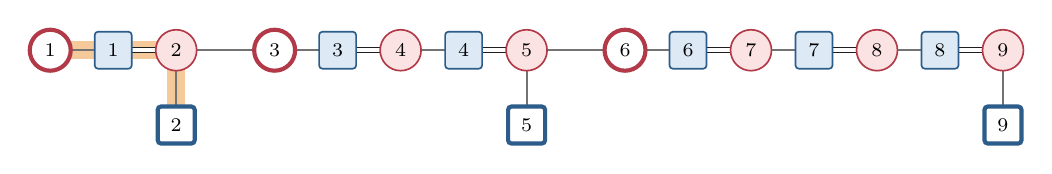
\begin{tikzpicture}[scale=1]
\begin{scope}[on background layer]
\draw[sap] (0.000,0.000) -- (0.800,0.000) -- (1.600,0.000) -- (1.600,-0.950);
\end{scope}
\draw[edge,draw=black!55,line width=.7pt] (0.000,0.000) -- (0.800,0.000);
\draw[couple] (1.600,0.000) -- (0.800,0.000);
\draw[edge,draw=black!55,line width=.7pt] (1.600,0.000) -- (1.600,-0.950);
\draw[edge,draw=black!55,line width=.7pt] (1.600,0.000) -- (3.650,0.000);
\draw[edge,draw=black!55,line width=.7pt] (2.850,0.000) -- (3.650,0.000);
\draw[couple] (4.450,0.000) -- (3.650,0.000);
\draw[edge,draw=black!55,line width=.7pt] (4.450,0.000) -- (5.250,0.000);
\draw[couple] (6.050,0.000) -- (5.250,0.000);
\draw[edge,draw=black!55,line width=.7pt] (6.050,0.000) -- (6.050,-0.950);
\draw[edge,draw=black!55,line width=.7pt] (6.050,0.000) -- (8.100,0.000);
\draw[edge,draw=black!55,line width=.7pt] (7.300,0.000) -- (8.100,0.000);
\draw[couple] (8.900,0.000) -- (8.100,0.000);
\draw[edge,draw=black!55,line width=.7pt] (8.900,0.000) -- (9.700,0.000);
\draw[couple] (10.500,0.000) -- (9.700,0.000);
\draw[edge,draw=black!55,line width=.7pt] (10.500,0.000) -- (11.300,0.000);
\draw[couple] (12.100,0.000) -- (11.300,0.000);
\draw[edge,draw=black!55,line width=.7pt] (12.100,0.000) -- (12.100,-0.950);
\node[girl,free] at (0.000,0.000) {1};
\node[girl] at (1.600,0.000) {2};
\node[girl,free] at (2.850,0.000) {3};
\node[girl] at (4.450,0.000) {4};
\node[girl] at (6.050,0.000) {5};
\node[girl,free] at (7.300,0.000) {6};
\node[girl] at (8.900,0.000) {7};
\node[girl] at (10.500,0.000) {8};
\node[girl] at (12.100,0.000) {9};
\node[boy] at (0.800,0.000) {1};
\node[boy,free] at (1.600,-0.950) {2};
\node[boy] at (3.650,0.000) {3};
\node[boy] at (5.250,0.000) {4};
\node[boy,free] at (6.050,-0.950) {5};
\node[boy] at (8.100,0.000) {6};
\node[boy] at (9.700,0.000) {7};
\node[boy] at (11.300,0.000) {8};
\node[boy,free] at (12.100,-0.950) {9};
\end{tikzpicture}

\caption{The tree for $K=4$ after~\Hs1, with the SAP of the first dag round.
Component $k$ is a path whose unique augmenting path has level~$k$; the
thin links between components never enter a dag.}
\label{fig:caterpillar}
\end{figure}

\begin{proposition}
On this tree Algorithm~H performs $K$ rounds. For $j=2,\ldots,K$ the
round at level~$L=j$ finds one SAP, which completes component~$j$, and
\[
   W_5=(2j-1)(K-j+1)+\Iv{j<K},\qquad W_{13}=j,\qquad W_{11}=j(K-j+1).
\]
In total $\sum W_5=K(K-1)(2K+5)/6+K-2$, $\sum W_{13}=K(K+1)/2-1$, and
$\sum W_{11}=K(K-1)(K+4)/6$, while~\Hs1 examines $s$ entries. Hence
$\sum W_5/(E\sqrt V)\to1/3$.
\end{proposition}

\begin{proof}
Step~\Hs1 scans each component's girls~$x_{k-1},\ldots,x_1$ before $x_0$ and
couples $x_i\db y_{i-1}$; it never reaches a link. So each component has a
single free girl~$x_0$ and a single free boy~$y_{k-1}$, its unique augmenting
path has level~$k$, and \A{QUEUE} lists the free girls from component $K$
down to component~2. The round at level~$j$ completes component $j$, whose
free girl is last in the queue, so step~\Hs{16} preserves the order.

The links do not interfere. A link goes from a girl of component $k$ to
the first boy of component $k+1$, so an alternating path, whose steps from
girls to boys follow edges, can only move to components of higher index.
In round~$j$ the free girls lie in components $j,\ldots,K$, so the
completed components $2,\ldots,j-1$ are never entered. The link out of
component $k$ starts at the girl~$x_{k-1}$, which lies at level~$k-1$; in
round~$j$ only levels up to $j-1$ are scanned, so this link is examined
only in round~$k$, and then its boy is already in $B_1$, so step~\Hs6
ignores it. Hence the dags are exactly those of the separate paths.

In round~$j$ each of the $K-j+1$ unresolved components contributes its
girls at levels~$0,\ldots,j-1$: one girl with one neighbour and $j-1$ with
two, $2j-1$ examinations in all, plus one for the link of component~$j$
if $j<K$. The shortest component is scanned last at every level, so the
boys at levels~$1,\ldots,j$ of all unresolved components are marked
before the free boy is found: $W_{11}=j(K-j+1)$. The only root is the free
boy of component~$j$, and its search consumes $j$ arcs.
\end{proof}

Here $\sum W_{13}=\Theta(E)$ but $\sum W_{11}=\Theta(E\sqrt V)$: the mark-resetting loop of
step~\Hs{11} is as expensive as the breadth-first search, and cannot be
left out of a running-time analysis.

\begin{remark}
Replacing component $k$ by a cycle $C_{4k-2}$, with suitable lists, gives a
2-regular graph with $s=K^2-1$ on which every round finds one SAP and
$\sum W_5/(E\sqrt V)\to1/(3\sqrt2)$. The staircase graphs do better on
both counts: they have the largest possible number of rounds, about
$2\sqrt s$, against about $\sqrt{2s}$ for the tree and $\sqrt s$ for the
cycles, and $\sum W_5/(E\sqrt V)\to2\sqrt2/3$
(Theorem~W).
\end{remark}

\section{Credits, literature, and open problems}
\label{sec:credits}

\subsection{Where the ideas come from}

\paragraph{Augmenting paths and phases.} The union of two matchings and the
$s-s'$ disjoint augmenting paths are due to Berge~\cite{Berge}. Hopcroft
and Karp~\cite{HK} introduced phases of vertex-disjoint shortest augmenting
paths. They proved that path lengths never decrease and that paths of one
length found in sequence are vertex-disjoint (their Theorem~2 and
Corollaries~3 and~4), and bounded the number of distinct lengths by
$2\floor{\sqrt s}+2$ (their Theorem~3), which gives running time
$O((V+E)\sqrt s)$ in our notation. The paper contains no lower-bound
example. Karzanov obtained the same bound independently~\cite{Karzanov}.
As the pre-fascicle notes on page~7, Dinitz's shortest-augmenting-path
algorithm for network flow, with improvements by Even and Itai, is
essentially the same procedure when specialized to bipartite matching
\cite{Dinitz2006}; see also Even and Tarjan~\cite{EvenTarjan}. On random
graphs long SAPs are rare, so the algorithm typically needs far fewer
rounds~\cite{Motwani,BMST}. Knuth's Algorithm~H, its
data structures, Theorem~H, Corollary~K, and exercises~5, 15, and~16 are in
\cite{Knuth}; Lemma~\ref{lem:15ab} is exercise~15(a,b) with Knuth's answer
spelled out.

\paragraph{Tchoukaillon numbers.} The sieve of exercise~12 and the numbers
$\Ch_n$ go back to Erdős and Jabotinsky~\cite{ErdosJabotinsky}, who studied
their growth; Broline and Loeb~\cite{BrolineLoeb} connected them with the
Tchoukaillon game and its $1/\pi$ asymptotics (Knuth's answer to
exercise~11 corrects an error bound claimed there); see also Jones, Taalman,
and Tongen~\cite{JTT} and OEIS sequence A002491~\cite{OEIS}. Exercise~11(d) gives $\Ch_n=n^2/\pi+O(n^{4/3})$, and Li
\cite{Li} has extended such asymptotics to the whole Tchoukaillon array.
Knuth's 2022 lecture~\cite{KnuthRutgers} linked Tchoukaillon numbers to the
question whether the Hopcroft--Karp algorithm can ever take nonlinear time.

\paragraph{Lower bounds on phases.} Hegerfeld and Kratsch
\cite{HegerfeldKratsch} study algorithms that follow the Hopcroft--Karp
phase framework, and show that such an algorithm \emph{may} need
$\Omega(\sqrt n)$ phases on paths, on trivially perfect graphs, and on
chain graphs, when the maximal set of SAPs removed in each phase is chosen
adversarially. Their constructions do not address whether a particular
implementation, with its own data structures, can be steered into those
choices by its input; Section~\ref{sec:order} shows that this can fail. On
graphs whose components have unique augmenting paths, such as the paths of
Section~\ref{sec:sparse}, every phase is forced, and examples of this kind
are folklore. We found no earlier statement of the exact value of $R(s)$.

\paragraph{New here.} As far as we know, the following are new: the exact
value of $R(s)$ and the staircase graphs (Theorems~R, S, and~W); the
comparison $Q_n\le\Ch_n$; the halving theorem and the classification of the
literal reading (Theorem~U, Corollary~L); and the results of
Section~\ref{sec:operational}. The upper bound in Theorem~R is a direct
refinement of the counting in Theorem~H and in~\cite{HK}. We would be
grateful to hear of earlier sources for any of these results.

\subsection{Open problems}

\begin{enumerate}
\item \textbf{The operational question.} Does every $s$ admit an ordered
  graph realizing the Tchoukaillon schedule? Even an infinite family of
  sizes would be progress. By Theorem~C such a family must have at least
  $s/12-O(1)$ independent cycles.
\item \textbf{The basic-row question.} The same, keeping $f$ disjoint SAPs
  in every round, as in Knuth's matrices. A positive answer implies one to
  the first question; by Section~\ref{sec:no-cover} a negative answer would
  not settle it. All computed examples (Appendix~\ref{app:catalog}) are
  basic-row.
\item \textbf{Most rounds from the largest start.} What is the largest number
  of rounds if~\Hs1 must leave $\floor{s/2}$ girls free? It is at most
  $R(s)$, and at least $T(s)$ for every $s$ at which the schedule can be
  realized; the staircase graphs start with only about $2\sqrt s$ free
  girls.
\item \textbf{Few edges.} How many edges does an operational realization
  need? Theorem~C gives $E\ge\frac{25}{12}s-O(1)$, using only two rounds.
\item \textbf{An explicit threshold.} Make explicit the size beyond which
  $R(s)>T(s)$ always holds; Section~\ref{sec:comparison} confirms it for
  $64\le s<3.2\times10^9$.
\end{enumerate}


\appendix
\section{An input order for Knuth's sixteen-pair graph}
\label{app:knuth16}

Answer~15(d) gives the graph but not an input order. Here is one under
which Algorithm~H follows the Tchoukaillon schedule and passes through
Knuth's matrices. We keep Knuth's logical names $g_k,b_k$. The edges are
$g_kb_k$ for $1\le k\le16$ and
\begin{equation}
\begin{gathered}
 b_1g_2,\ b_3g_4,\ b_5g_6,\ \ldots,\ b_{15}g_{16},\\
 b_2g_4,\ b_3g_5,\ b_8g_{10},\ b_9g_{11},\ b_{14}g_{16},\
 b_4g_6,\ b_5g_8,\ b_7g_9,\ b_6g_{10},\ b_3g_7,\ b_{10}g_{12},
\end{gathered}
\label{eq:knuth16edges}
\end{equation}
so $M=N=s=16$ and $E=35$.

\paragraph{The input.} Throughout this appendix $g_k$ and $b_k$ are Knuth's
logical names; the numbers that Algorithm~H sees as girl indices are a
separate thing, given in the column ``number'' below. Boys keep their
numbers. Girls receive the numbers $16,15,\ldots,1$ in the order
\[
  g_{16},g_{14},g_{12},g_{10},g_8,g_6,g_4,g_2,\ g_1,g_3,g_7,g_{13},g_9,g_{15},g_{11},g_5 .
\]
Each girl's list is in increasing order of boys, except that an even girl
$g_k$ puts $b_{k-1}$ first. In numerical form:
\begin{center}\small
\begin{tabular}{rrl@{\qquad}rrl}
\toprule
number&girl&list&number&girl&list\\
\midrule
1&$g_5$&$[3,5]$&9&$g_2$&$[1,2]$\\
2&$g_{11}$&$[9,11]$&10&$g_4$&$[3,2,4]$\\
3&$g_{15}$&$[15]$&11&$g_6$&$[5,4,6]$\\
4&$g_9$&$[7,9]$&12&$g_8$&$[7,5,8]$\\
5&$g_{13}$&$[13]$&13&$g_{10}$&$[9,6,8,10]$\\
6&$g_7$&$[3,7]$&14&$g_{12}$&$[11,10,12]$\\
7&$g_3$&$[3]$&15&$g_{14}$&$[13,14]$\\
8&$g_1$&$[1]$&16&$g_{16}$&$[15,14,16]$\\
\bottomrule
\end{tabular}
\end{center}

\paragraph{The run.} Step~\Hs1 scans the even girls first; each takes
$b_{k-1}$, so the matching is $b_1g_2$, $b_3g_4$, \dots, $b_{15}g_{16}$, as in
Knuth's first matrix, and~\Hs1 examines 20 entries. The rounds are:
\begin{center}\small
\begin{tabular}{crrrrrl}
\toprule
$L$&$f$&SAPs&$W_5$&$W_{13}$&$W_{11}$&SAPs found, as new couples $(g,b)$\\
\midrule
2&8&3&35&16&16&$(5,3),(4,2)$;\ $(11,9),(10,8)$;\ $(15,15),(16,14)$\\
3&5&2&34&14&15&$(9,7),(8,5),(6,4)$;\ $(13,13),(14,14),(16,16)$\\
4&3&1&28&10&12&$(7,3),(5,5),(8,8),(10,6)$\\
5&2&1&25&6&12&$(3,3),(7,7),(9,9),(11,11),(12,10)$\\
6&1&1&24&6&12&$(1,1),(2,2),(4,4),(6,6),(10,10),(12,12)$\\
\bottomrule
\end{tabular}
\end{center}
Here girls have their logical names. The free girls before the rounds are,
in \A{QUEUE} order, $(1,3,7,13,9,15,11,5)$, $(1,3,7,13,9)$, $(1,3,7)$,
$(1,3)$, $(1)$; every SAP ends at the last free girl, so step~\Hs{16} never
reorders the queue. After each round the basic paths with respect to the
matching $g_kb_k$ are exactly the rows of the next matrix in
Fig.~\ref{fig:knuth16rows}, and the run ends with that perfect matching.

\paragraph{All augmenting paths.} Enumerating every simple augmenting path
before each round gives the following counts, by level.
\begin{center}\small
\begin{tabular}{cl}
\toprule
before the round at&numbers of augmenting paths of each level\\
\midrule
$L=2$&22 of level~2, 4 of level~3\\
$L=3$&16 of level~3, 6 of level~5\\
$L=4$&7 of level~4, 12 of level~6, 8 of level~8\\
$L=5$&3 of level~5, 4 of level~7, 4 of level~9, 2 of level~11\\
$L=6$&1 of level~6\\
\bottomrule
\end{tabular}
\end{center}
So property $\Up$ fails in every round but the last, while property
$\Bp$ holds throughout. The paths $\pi_2$ and $\pi_3$ of~\eqref{eq:PQ} are two of
the 26 counted in the first line.

\section{The halving graphs}
\label{app:halving}

These graphs show that Theorem~U is sharp and supply the literal examples
in Corollary~L. Let $f=2^t$ with $t\ge0$. For a positive integer~$i$ let
$\rho(i)$ be the exponent of the largest power of~2 that divides~$i$ (the
``ruler function''; for example $\rho(12)=2$). The graph has girls~$u_i,c_i$
and boys~$b_i,d_i$ for $1\le i\le f$, and the edges
\[
  u_ib_i,\quad c_ib_i,\quad c_id_i\quad(1\le i\le f),\qquad
  u_i\,b_{i+2^{\rho(i)}}\quad(1\le i<f).
\]
So $M=N=s=2f$ and $E=4f-1$; the edges $u_ib_i$ and $c_id_i$ form a perfect
matching.

\paragraph{The input.} Number $b_i$ as $2i-1$ and $d_i$ as $2i$, and number
$c_i$ as $f+i$, with list $[b_i,d_i]$. Sort the indices~$i$ by decreasing
$\rho(i)$, breaking ties by increasing~$i$, and give the corresponding
girls~$u_i$ the numbers $f,f-1,\ldots,1$ in that order. The list of $u_i$ is
$[b_i,b_{i+2^{\rho(i)}}]$, or $[b_f]$ when $i=f$. For the three literal
examples of Corollary~L this gives
\begin{center}\small
\begin{tabular}{cl}
\toprule
$s$&girl lists, in increasing order of girls\\
\midrule
2&$[1];\ [1,2]$\\
4&$[1,3];\ [3];\ [1,2];\ [3,4]$\\
8&$[5,7];\ [1,3];\ [3,7];\ [7];\ [1,2];\ [3,4];\ [5,6];\ [7,8]$\\
\bottomrule
\end{tabular}
\end{center}

\paragraph{The run.} Step~\Hs1 couples every $c_i$ with $b_i$ and leaves all
$u_i$ free, in the order just described. After $r$ dag rounds
($0\le r\le t$) the free girls are the $u_i$ with $2^r\mid i$, and the
indices fall into \emph{blocks} of $2^r$ consecutive integers
$i-2^r<j\le i$, one block for each free girl~$u_i$. Her basic path visits
$r+1$ of the girls~$u_j$ of her block, namely $u_i$ and then $u_j$ for
$j=i-2^r+2^q$ with $q=r-1,\ldots,1,0$, and ends with $c\sg d$ at the
smallest index of the block; it has level~$r+2$. For example, when $f=4$
and $r=1$ the free girls are $u_2$ and $u_4$, and the basic path of $u_4$
is $u_4\sg b_4\db u_3\sg b_3\db c_3\sg d_3$.

Every augmenting path has level~$r+2$ at this stage: a free girl can start
along $b_i$ or along $b_{i+2^{\rho(i)}}$, and after that first step the
alternating continuation is forced. In the next round step~\Hs6 lists, at
each $b_i$, the free girls in reverse queue order. As a result the search
joins each block whose free girl~$u_i$ has $\rho(i)=r$ to the block on its
right; the other roots fail at deleted girls; and step~\Hs{16} removes
exactly the girls with $\rho(i)=r$, which form the end of the queue. So the
free girls go $f\to f/2\to\cdots\to1\to0$ in $t+1$ dag rounds, and
property~$\Up$ holds in every round. (For $f\le32$ we have also checked
this by simulation, including a census of all augmenting paths.)

\paragraph{Work.} The round that starts with $n'=f/2^r$ free girls has
$W_5=2n'(r+2)-1$ and $W_{13}=W_{11}=n'(r+2)$; in total
$\sum W_5=12f-3t-9$ and $\sum W_{13}=\sum W_{11}=6f-t-4$, and~\Hs1 examines
$3f-1$ entries. So these graphs need only linear work in all.

\section{Computed realizations for small sizes}
\label{app:catalog}

For every even $s=2h\le40$ the search described in
Section~\ref{sec:catalog} found an ordered graph that realizes the
Tchoukaillon schedule; by Proposition~\ref{prop:odd} this covers all
$s\le41$. In each example~\Hs1 produces the matching
$g_{h+j}\db b_{2j-1}$ ($1\le j\le h$) and leaves girls~$h,h-1,\ldots,1$ free,
in that order. The table gives the number of edges, the number of rounds
(counting~\Hs1), the work counts summed over all rounds after~\Hs1, and the
numbers of SAPs removed at levels~$2,3,\ldots$. The entry for $s=16$ is
Knuth's graph with the input of Appendix~\ref{app:knuth16}. The complete
ordered lists are in the file \texttt{code/data/numerical\_witnesses.json},
and \texttt{python algorithm\_h.py catalog $s$ -{}-json} prints every queue,
dag, and SAP of the run on any of them (Appendix~\ref{app:code}).

\begin{center}\small
\setlength{\tabcolsep}{5pt}
\begin{tabular}{rrrrrrrl}
\toprule
$s$&$E$&rounds&\Hs1&$W_5$&$W_{13}$&$W_{11}$&SAPs removed\\
\midrule
2&3&2&2&3&2&2&$1$\\
4&7&3&5&12&7&7&$1,1$\\
6&12&4&7&34&14&18&$1,1,1$\\
8&15&4&9&37&16&20&$2,1,1$\\
10&21&5&13&67&29&33&$2,1,1,1$\\
12&28&6&16&133&46&60&$2,1,1,1,1$\\
14&31&6&19&123&49&56&$3,1,1,1,1$\\
16&35&6&20&146&52&67&$3,2,1,1,1$\\
18&43&7&25&212&77&93&$3,2,1,1,1,1$\\
20&46&7&27&223&78&97&$4,2,1,1,1,1$\\
22&55&8&30&367&109&148&$4,2,1,1,1,1,1$\\
24&60&8&34&378&117&156&$4,2,2,1,1,1,1$\\
26&63&8&39&362&118&149&$5,2,2,1,1,1,1$\\
28&67&8&39&363&121&150&$5,3,2,1,1,1,1$\\
30&77&9&45&515&164&208&$5,3,2,1,1,1,1,1$\\
32&79&9&47&542&164&221&$6,3,2,1,1,1,1,1$\\
34&91&10&55&709&214&270&$6,3,2,1,1,1,1,1,1$\\
36&97&10&56&748&224&285&$6,3,2,2,1,1,1,1,1$\\
38&100&10&58&779&220&299&$7,3,2,2,1,1,1,1,1$\\
40&104&10&61&716&225&272&$7,4,2,2,1,1,1,1,1$\\
\bottomrule
\end{tabular}
\end{center}

\section{Programs and checks}
\label{app:code}

The proofs in these notes do not depend on computation. The programs make
the examples checkable and catch mistakes. They are in the directory
\texttt{code/} of the repository
\href{https://github.com/boonsuan/hopcroftkarp}{github.com/boonsuan/hopcroftkarp},
and need only Python~3.10 or later and its standard library (NumPy is used
only by the longest check).

\paragraph{Simulators.} \texttt{algorithm\_h.py} is a literal transcription
of Algorithm~H: it builds the edge nodes as in answer~6, runs step~\Hs1 as in
answer~7, and runs steps \Hs2--\Hs{17} under an explicit program counter. It
records every queue, \A{MARKED} order, \A{BLINK} list, SAP, and the counts
$W_5$, $W_{13}$, $W_{11}$. \texttt{independent\_audit.py} implements the same
rules with ordinary loops and lists and shares no code with it; the two must
produce identical records. \texttt{augmenting.py} contains computations that
do not use Algorithm~H at all: maximum matchings by plain augmenting paths, an
exhaustive list of augmenting paths for small graphs, and $\nu$ by a max-flow
computation.

\paragraph{Examples and figures.} \texttt{examples.py} builds every named
graph of these notes (the staircase graphs $\Gam_n$ and their padding to any
$s$, Knuth's 16-pair graph with the input of Appendix~\ref{app:knuth16}, the
8-pair tree, the halving, caterpillar, six-pair, and triangular chain graphs,
and the catalog of Appendix~\ref{app:catalog}), together with the schedule
and the numbers $T(s)$, $R(s)$, $Q_n$, $\Ch_n$. \texttt{make\_figures.py}
draws every figure that shows a matching, dag, or SAP of a specific graph
by running the simulator, so the pictures show exactly what Algorithm~H does.

\paragraph{Search.} \texttt{search.py} is the search of
Section~\ref{sec:catalog}. For each even $s$ it builds an ordered graph one
round of the Tchoukaillon schedule at a time, rerunning Algorithm~H
from~\Hs1 after every proposed change, and replays what it finds with both
simulators. Its random choices are seeded, so every run finds the same
graphs; they are written to \texttt{code/data/search\_results.json}. The
module's documentation describes the method in full.

\paragraph{Checks.} \texttt{verify.py} runs fifteen named checks, one for
each group of computed statements in these notes, and prints a pass/fail line
for each. They include the hook description of Lemma~\ref{lem:hooks} and the
search of Lemmas~\ref{lem:bfs} and~\ref{lem:dfs} for $n\le60$, the count
$2^m-1$ of SAPs (by exhaustive enumeration for $n\le9$), the counts of
Theorem~W, the padding to every size, the claim about the corner edge in
Section~\ref{sec:gamma}, the values of $\Ch_n$ and the comparison with $Q_n$,
the replay of every example and table, $\nu=f$ in the catalog and in the
graphs found by \texttt{search.py}, the tree of
Section~\ref{sec:no-cover}, and the six-pair and chain obstructions.

\paragraph{Reproducing.} From \texttt{code/}:
\begin{center}
\begin{tabular}{ll}
\texttt{python verify.py} & all checks, about 11 seconds\\
\texttt{python verify.py -{}-full} & full ranges, including $\Ch_n$ for $n\le10^5$\\
& and all 103680 six-pair inputs (about 40 seconds)\\
\texttt{python make\_figures.py} & redraws \texttt{report/figures/gen\_*}\\
\texttt{python search.py 46} & searches every even $s\le46$ (about two minutes)\\
\texttt{python algorithm\_h.py gamma 5} & prints a run (try \texttt{-{}-help})
\end{tabular}
\end{center}
and from \texttt{report/}, two runs of \texttt{pdflatex main.tex} build these
notes. The website \href{https://hopcroftkarp.site}{hopcroftkarp.site} has its own port of the
simulator, tested step by step against traces exported from
\texttt{algorithm\_h.py}.


\begin{thebibliography}{99}
\small

\bibitem{Berge}
Claude Berge, ``Two theorems in graph theory,'' \emph{Proceedings of the
National Academy of Sciences of the USA} \textbf{43} (1957), 842--844.
\href{https://doi.org/10.1073/pnas.43.9.842}{doi:10.1073/pnas.43.9.842}.

\bibitem{BMST}
Holger Bast, Kurt Mehlhorn, Guido Schäfer, and Hisao Tamaki, ``Matching
algorithms are fast in sparse random graphs,'' \emph{Theory of Computing
Systems} \textbf{39} (2006), 3--14.

\bibitem{BrolineLoeb}
Duane M. Broline and Daniel E. Loeb, ``The combinatorics of Mancala-type
games: Ayo, Tchoukaillon, and $1/\pi$,'' \emph{UMAP Journal} \textbf{16}
(1995), 21--36. \href{https://arxiv.org/abs/math/9502225}{arXiv:math/9502225}.

\bibitem{Dinitz2006}
Yefim Dinitz, ``Dinitz' algorithm: The original version and Even's
version,'' in \emph{Theoretical Computer Science: Essays in Memory of Shimon
Even}, Lecture Notes in Computer Science \textbf{3895} (2006), 218--240.
\href{https://doi.org/10.1007/11685654_10}{doi:10.1007/11685654\_10}.

\bibitem{ErdosJabotinsky}
Paul Erdős and Eri Jabotinsky, ``On sequences of integers generated by a
sieving process,'' \emph{Indagationes Mathematicae} \textbf{20} (1958),
115--128.

\bibitem{EvenTarjan}
Shimon Even and Robert Endre Tarjan, ``Network flow and testing graph
connectivity,'' \emph{SIAM Journal on Computing} \textbf{4} (1975), 507--518.

\bibitem{HegerfeldKratsch}
Falko Hegerfeld and Stefan Kratsch, ``On adaptive algorithms for maximum
matching,'' \emph{46th International Colloquium on Automata, Languages, and
Programming (ICALP 2019)}, LIPIcs \textbf{132} (2019), 71:1--71:16.
\href{https://doi.org/10.4230/LIPIcs.ICALP.2019.71}{doi:10.4230/LIPIcs.ICALP.2019.71};
\href{https://arxiv.org/abs/1904.11244}{arXiv:1904.11244}.

\bibitem{HK}
John E. Hopcroft and Richard M. Karp, ``An $n^{5/2}$ algorithm for maximum
matchings in bipartite graphs,'' \emph{SIAM Journal on Computing} \textbf{2}
(1973), 225--231.
\href{https://doi.org/10.1137/0202019}{doi:10.1137/0202019}.

\bibitem{JTT}
Brant Jones, Laura Taalman, and Anthony Tongen, ``Solitaire mancala games and
the Chinese remainder theorem,'' \emph{American Mathematical Monthly}
\textbf{120} (2013), 706--724.
\href{https://arxiv.org/abs/1112.3593}{arXiv:1112.3593}.

\bibitem{Karzanov}
A. V. Karzanov, ``An exact estimate of an algorithm for finding a maximum
flow, applied to the problem on representatives'' (in Russian), in
\emph{Problems in Cybernetics: Proceedings of the Seminar on Combinatorial
Mathematics}, Moscow, 1973, 66--70.

\bibitem{Knuth}
Donald E. Knuth, \emph{The Art of Computer Programming}, Volume~4,
Pre-Fascicle~14A: \emph{Bipartite Matching}, Section~7.5.1. Draft of
18 September 2026 (zeroth printing, revision~$-88$). Page numbers in these
notes refer to this draft.

\bibitem{KnuthRutgers}
Donald E. Knuth, ``Tchoukaillon numbers,'' Rutgers Experimental Mathematics
Seminar, 27 January 2022. Abstract at
\href{https://dimacs.rutgers.edu/dimacsevents/seminar-details/tchoukaillon-numbers}{dimacs.rutgers.edu};
video at \href{https://vimeo.com/672468553}{vimeo.com/672468553}.

\bibitem{Li}
Shisheng Li, ``Asymptotics of the Tchoukaillon array and a conjecture of
Beluhov,'' 2026. \href{https://arxiv.org/abs/2608.17517}{arXiv:2608.17517}.

\bibitem{Motwani}
Rajeev Motwani, ``Average-case analysis of algorithms for matchings and
related problems,'' \emph{Journal of the ACM} \textbf{41} (1994), 1329--1356.

\bibitem{OEIS}
OEIS Foundation, \emph{The On-Line Encyclopedia of Integer Sequences},
sequence A002491. \href{https://oeis.org/A002491}{oeis.org/A002491}.

\end{thebibliography}


\end{document}
